% Options for packages loaded elsewhere
\PassOptionsToPackage{unicode}{hyperref}
\PassOptionsToPackage{hyphens}{url}
%
\documentclass[
]{book}
\usepackage{amsmath,amssymb}
\usepackage{iftex}
\ifPDFTeX
  \usepackage[T1]{fontenc}
  \usepackage[utf8]{inputenc}
  \usepackage{textcomp} % provide euro and other symbols
\else % if luatex or xetex
  \usepackage{unicode-math} % this also loads fontspec
  \defaultfontfeatures{Scale=MatchLowercase}
  \defaultfontfeatures[\rmfamily]{Ligatures=TeX,Scale=1}
\fi
\usepackage{lmodern}
\ifPDFTeX\else
  % xetex/luatex font selection
\fi
% Use upquote if available, for straight quotes in verbatim environments
\IfFileExists{upquote.sty}{\usepackage{upquote}}{}
\IfFileExists{microtype.sty}{% use microtype if available
  \usepackage[]{microtype}
  \UseMicrotypeSet[protrusion]{basicmath} % disable protrusion for tt fonts
}{}
\makeatletter
\@ifundefined{KOMAClassName}{% if non-KOMA class
  \IfFileExists{parskip.sty}{%
    \usepackage{parskip}
  }{% else
    \setlength{\parindent}{0pt}
    \setlength{\parskip}{6pt plus 2pt minus 1pt}}
}{% if KOMA class
  \KOMAoptions{parskip=half}}
\makeatother
\usepackage{xcolor}
\usepackage{color}
\usepackage{fancyvrb}
\newcommand{\VerbBar}{|}
\newcommand{\VERB}{\Verb[commandchars=\\\{\}]}
\DefineVerbatimEnvironment{Highlighting}{Verbatim}{commandchars=\\\{\}}
% Add ',fontsize=\small' for more characters per line
\usepackage{framed}
\definecolor{shadecolor}{RGB}{248,248,248}
\newenvironment{Shaded}{\begin{snugshade}}{\end{snugshade}}
\newcommand{\AlertTok}[1]{\textcolor[rgb]{0.94,0.16,0.16}{#1}}
\newcommand{\AnnotationTok}[1]{\textcolor[rgb]{0.56,0.35,0.01}{\textbf{\textit{#1}}}}
\newcommand{\AttributeTok}[1]{\textcolor[rgb]{0.13,0.29,0.53}{#1}}
\newcommand{\BaseNTok}[1]{\textcolor[rgb]{0.00,0.00,0.81}{#1}}
\newcommand{\BuiltInTok}[1]{#1}
\newcommand{\CharTok}[1]{\textcolor[rgb]{0.31,0.60,0.02}{#1}}
\newcommand{\CommentTok}[1]{\textcolor[rgb]{0.56,0.35,0.01}{\textit{#1}}}
\newcommand{\CommentVarTok}[1]{\textcolor[rgb]{0.56,0.35,0.01}{\textbf{\textit{#1}}}}
\newcommand{\ConstantTok}[1]{\textcolor[rgb]{0.56,0.35,0.01}{#1}}
\newcommand{\ControlFlowTok}[1]{\textcolor[rgb]{0.13,0.29,0.53}{\textbf{#1}}}
\newcommand{\DataTypeTok}[1]{\textcolor[rgb]{0.13,0.29,0.53}{#1}}
\newcommand{\DecValTok}[1]{\textcolor[rgb]{0.00,0.00,0.81}{#1}}
\newcommand{\DocumentationTok}[1]{\textcolor[rgb]{0.56,0.35,0.01}{\textbf{\textit{#1}}}}
\newcommand{\ErrorTok}[1]{\textcolor[rgb]{0.64,0.00,0.00}{\textbf{#1}}}
\newcommand{\ExtensionTok}[1]{#1}
\newcommand{\FloatTok}[1]{\textcolor[rgb]{0.00,0.00,0.81}{#1}}
\newcommand{\FunctionTok}[1]{\textcolor[rgb]{0.13,0.29,0.53}{\textbf{#1}}}
\newcommand{\ImportTok}[1]{#1}
\newcommand{\InformationTok}[1]{\textcolor[rgb]{0.56,0.35,0.01}{\textbf{\textit{#1}}}}
\newcommand{\KeywordTok}[1]{\textcolor[rgb]{0.13,0.29,0.53}{\textbf{#1}}}
\newcommand{\NormalTok}[1]{#1}
\newcommand{\OperatorTok}[1]{\textcolor[rgb]{0.81,0.36,0.00}{\textbf{#1}}}
\newcommand{\OtherTok}[1]{\textcolor[rgb]{0.56,0.35,0.01}{#1}}
\newcommand{\PreprocessorTok}[1]{\textcolor[rgb]{0.56,0.35,0.01}{\textit{#1}}}
\newcommand{\RegionMarkerTok}[1]{#1}
\newcommand{\SpecialCharTok}[1]{\textcolor[rgb]{0.81,0.36,0.00}{\textbf{#1}}}
\newcommand{\SpecialStringTok}[1]{\textcolor[rgb]{0.31,0.60,0.02}{#1}}
\newcommand{\StringTok}[1]{\textcolor[rgb]{0.31,0.60,0.02}{#1}}
\newcommand{\VariableTok}[1]{\textcolor[rgb]{0.00,0.00,0.00}{#1}}
\newcommand{\VerbatimStringTok}[1]{\textcolor[rgb]{0.31,0.60,0.02}{#1}}
\newcommand{\WarningTok}[1]{\textcolor[rgb]{0.56,0.35,0.01}{\textbf{\textit{#1}}}}
\usepackage{longtable,booktabs,array}
\usepackage{calc} % for calculating minipage widths
% Correct order of tables after \paragraph or \subparagraph
\usepackage{etoolbox}
\makeatletter
\patchcmd\longtable{\par}{\if@noskipsec\mbox{}\fi\par}{}{}
\makeatother
% Allow footnotes in longtable head/foot
\IfFileExists{footnotehyper.sty}{\usepackage{footnotehyper}}{\usepackage{footnote}}
\makesavenoteenv{longtable}
\usepackage{graphicx}
\makeatletter
\def\maxwidth{\ifdim\Gin@nat@width>\linewidth\linewidth\else\Gin@nat@width\fi}
\def\maxheight{\ifdim\Gin@nat@height>\textheight\textheight\else\Gin@nat@height\fi}
\makeatother
% Scale images if necessary, so that they will not overflow the page
% margins by default, and it is still possible to overwrite the defaults
% using explicit options in \includegraphics[width, height, ...]{}
\setkeys{Gin}{width=\maxwidth,height=\maxheight,keepaspectratio}
% Set default figure placement to htbp
\makeatletter
\def\fps@figure{htbp}
\makeatother
\setlength{\emergencystretch}{3em} % prevent overfull lines
\providecommand{\tightlist}{%
  \setlength{\itemsep}{0pt}\setlength{\parskip}{0pt}}
\setcounter{secnumdepth}{5}
\usepackage{booktabs}
\usepackage{amsthm}
\makeatletter

\newenvironment{kframe}{%
\medskip{}
\setlength{\fboxsep}{.8em}
 \def\at@end@of@kframe{}%
 \ifinner\ifhmode%
  \def\at@end@of@kframe{\end{minipage}}%
  \begin{minipage}{\columnwidth}%
 \fi\fi%
 \def\FrameCommand##1{\hskip\@totalleftmargin \hskip-\fboxsep
 \colorbox{shadecolor}{##1}\hskip-\fboxsep
     % There is no \\@totalrightmargin, so:
     \hskip-\linewidth \hskip-\@totalleftmargin \hskip\columnwidth}%
 \MakeFramed {\advance\hsize-\width
   \@totalleftmargin\z@ \linewidth\hsize
   \@setminipage}}%
 {\par\unskip\endMakeFramed%
 \at@end@of@kframe}
\makeatother

\makeatletter
\@ifundefined{Shaded}{
}{\renewenvironment{Shaded}{\begin{kframe}}{\end{kframe}}}
\makeatother

\newenvironment{block}[1]
  {
  \begin{itemize}
  \renewcommand{\labelitemi}{
    \raisebox{-.7\height}[0pt][0pt]{
      {\setkeys{Gin}{width=3em,keepaspectratio}\includegraphics{images/#1}}
    }
  }
  \setlength{\fboxsep}{1em}
  \begin{kframe}
  \item
  }
  {
  \end{kframe}
  \end{itemize}
  }
\newenvironment{rmdnote}
  {\begin{block}{note}}
  {\end{block}}
\newenvironment{rmdtip}
  {\begin{block}{tip}}
  {\end{block}}
\newenvironment{rmdquestion}
  {\begin{block}{question}}
  {\end{block}}
\newenvironment{rmdwarning}
  {\begin{block}{warning}}
  {\end{block}}
  
\def\thm@space@setup{%
  \thm@preskip=8pt plus 2pt minus 4pt
  \thm@postskip=\thm@preskip
}
\makeatother
\ifLuaTeX
  \usepackage{selnolig}  % disable illegal ligatures
\fi
\IfFileExists{bookmark.sty}{\usepackage{bookmark}}{\usepackage{hyperref}}
\IfFileExists{xurl.sty}{\usepackage{xurl}}{} % add URL line breaks if available
\urlstyle{same}
\hypersetup{
  pdftitle={Introduction to Data Science - BIO-4008Y/CHE-4602Y},
  pdfauthor={Dr Ellen Bell},
  hidelinks,
  pdfcreator={LaTeX via pandoc}}

\title{Introduction to Data Science - BIO-4008Y/CHE-4602Y}
\author{Dr Ellen Bell}
\date{2023-09-20}

\begin{document}
\maketitle

{
\setcounter{tocdepth}{1}
\tableofcontents
}
\hypertarget{welcome-to-the-data-science-workbook}{%
\chapter{Welcome to the Data Science Workbook}\label{welcome-to-the-data-science-workbook}}

\hypertarget{data-science-learning-objectives}{%
\section{Data Science learning objectives}\label{data-science-learning-objectives}}

Introduction to Data Science is a `sub-module' that will run throughout your first year as part of the BIO-4008Y anc CHE-4602Y Skills modules. Here we aim to teach you the fundamentals of how to collect and organise data in a clean and sensible format and how to correctly visualise and describe data. The platform we will be using to manage, manipulate and analyse data is posit Cloud. This is a cloud based interface that utilises the programming language R in a very similar interface to RStudio (a package you may wish to install on your own computers at some point). Over the course of the next few weeks you will start to learn fundamentals of this language and its application in posit Cloud.

\hypertarget{teaching-layout-for-data-science}{%
\section{Teaching layout for Data Science}\label{teaching-layout-for-data-science}}

In Semester 1 we will be learning some basic R syntax, how to create and load data sets and how to produce some basic data visualisations that are attractive and reproducible. Each week you will have either a lecture or a 1 hour workshop, you will also be expected to complete a chapter of this workbook each week, in your own time.

Teaching for semester 1;

\begin{itemize}
\tightlist
\item
  Semester 1 Lectures - Weeks; 2, 3, 6, 7, 9, 10
\item
  Semester 1 Workshops - Weeks; 4, 8, 11
\end{itemize}

In semester 2 will move onto some slightly more advanced data interpretation and visualisation skills and some descriptive statistics. Towards the end of the module we will briefly touch on inferential statistics, but this will be a very brief introduction. You will have a lecture every week until week 8 and a 2 hour workshop every other week. The workshops are all outlined as chapters in this workbook, if you don't complete a workshop in the timetabled slot, we strongly recommend you make every effort to complete it in your own time.

Teaching for semester 2;

\begin{itemize}
\tightlist
\item
  Semester 2 Lectures - Weeks; 1, 2, 3, 4, 5, 6, 7, 8
\item
  Semester 2 Workshops - Weeks; 2, 4, 6, 8
\end{itemize}

\hypertarget{assessment}{%
\section{Assessment}\label{assessment}}

\begin{itemize}
\tightlist
\item
  Semester 1
\end{itemize}

At the end of Semester 1 you will be given the opportunity to submit a formative assignment. From this you will get feedback and a mock grade for your work, the formative assignment and marking scheme is similar to the the later summative assignment (in Semester 2) so is a great opportunity to get constructive feedback on your work and places to improve on.

\begin{itemize}
\tightlist
\item
  Semester 2
\end{itemize}

During Semester 2 you will be given an assessment data set and a series of questions, you will be asked to produce a series of plots and format them into a multi-panel figure with accompanying figure legend. You will be asked to upload these alongside your R script and these will constitute the summative task for the Data Sciences component of your respective skills module.

\hypertarget{how-to-use-this-workbook}{%
\section{How to use this workbook}\label{how-to-use-this-workbook}}

In semester 1 each week of taught material is accompanied by a workbook chapter. You will be expected to read through these chapters and complete any exercises in your own time. Each chapter should take no more then an hour to complete and in many cases will take much less time. I will aim to set aside 10 minutes at the end of each lecture to cover any potential problems you may be having, so if you get stuck, use this time to ask for help. In semester 2 we have more face to face workshop time, in each workshop you will be expected to work through a chapter in this workbook, you may not complete this in the allocated time, but will be expected to do so in your own time. Use face to face time to ask lots of questions, especially if you are stuck.

\hypertarget{why-is-data-science-important-and-why-are-we-teaching-it-in-r}{%
\section{Why is data science important and why are we teaching it in R?}\label{why-is-data-science-important-and-why-are-we-teaching-it-in-r}}

It is a common misconception, that to be a good biologist or biochemist you need to `know' the mechanics of how life works. Questions like; ``How does a cell undergo respiration?'', ``How do kidneys filter blood?'', ``How do some plants fix nitrogen?'' and ``How do honey bees communicate the location and quantity of resources to each other?'', spring to mind. While these questions are important, they are also, now, fairly well understood. But how did biologists come to their understanding of these mechanisms? The answer to this lies in data.

Good science is based on empirical observations and these observations should be reliably collected and reproducible. Exploration of theories through observations and experimentation leads to the collection of data and analysis and interpretation of data feeds into the bedrock of our understanding of how life works, i.e.~the biological sciences.

Hopefully you can see why data handling, analysis and interpretation are important. So why are we teaching you how to handle data using R?

To many of you the use of programming languages, such as R, will be new. However if you can get into the habit of manipulating and analysing data in R you will be well set on the path to becoming an efficient and effective data analyst. Being confident with data is a key skill in the sciences and will serve you well in many career paths. In addition, knowledge and experience of programming languages such as R are fast becoming key skills in their own right, in science, industry, government and beyond.

In terms of the use of R for data handling and analysis, you may notice that the term \textbf{reproducible} reoccurs throughout this workbook. In the same way that your methods of data collection should be conducted and recorded in such a way that they may be reproduced by others, your data manipulation and analysis must also be conducted and recorded so as to be reproducible. Using R within the posit Cloud interface (we will come back to this in Chapter 2) makes it easy to record your data manipulation and analysis workflow and, if done well, makes it very easy for others to see and repeat what you have done.

So hopefully I have convinced you that data handling, analysis and R are all worthwhile skills to cultivate. We will spend some time in lectures discussing this as well. But for now take a look at Chapter 2. Happy coding!

\hypertarget{introduction-to-r-and-posit-cloud---week-2a}{%
\chapter{Introduction to R and posit Cloud - Week 2A}\label{introduction-to-r-and-posit-cloud---week-2a}}

You should aim to complete this chapter in Week 2, Semester 1.

\hypertarget{what-is-r-and-posit-cloud}{%
\section{What is R and posit Cloud?}\label{what-is-r-and-posit-cloud}}

So hopefully you have read through Chapter 1, where R and the posit Cloud interface were introduced in this module. But what really is R and what is the difference between R and posit Cloud?

Essentially R is a programming language that is commonly used in statistical computing, data handling, data visualisation and data analysis. Posit Cloud is a cloud based interface for a piece of software called RStudio (we wont be using the non cloud based RStudio in this sub-module, so we wont explore this software further here). Posit Cloud uses the R programming language but has a nice user friendly interface and is a great tool for learning how to conduct analysis in R.

We are using the posit cloud rather then RStudio because it means that no one has to worry about installing extra software on their own computers and everyone will be working with the same software versions. You will all need to create your own free accounts on posit Cloud, but first have a look at the short video below introducing you to the interface.

Now that you've watched the video, create your own Free posit Cloud account \href{https://login.rstudio.cloud/login?redirect=\%2Foauth\%2Fauthorize\%3Fredirect_uri\%3Dhttps\%253A\%252F\%252Frstudio.cloud\%252Flogin\%26client_id\%3Drstudio-cloud\%26response_type\%3Dcode\%26show_auth\%3D0\%26show_login\%3D1}{here}.

\hypertarget{a-warning-on-managing-your-work-flow}{%
\section{A warning on managing your work flow}\label{a-warning-on-managing-your-work-flow}}

Your free posit Cloud account comes with some restrictions which you should be aware of. These are;

\begin{itemize}
\tightlist
\item
  You may have up to 50 projects in total
\item
  You are limited to 25 project hours per month
\item
  You have up to 1GB of RAM and 1 CPU per project
\end{itemize}

For the purposes of our work here these restrictions should not be a problem. But I strongly suggest you don't leave your coursework to the last minute. If you try and pack in a whole semester or years worth or material into a single month, you will exceed those 25 project hours. There are some options of last resort should this happen, you could install RStudio on your desktop for example, or set up an alternative posit cloud account with an alternative email address, but things will get complicated. Lets avoid that where we can! There are some ways you can increase the efficiency of your workspace which are documented below in section 2.4.

\hypertarget{creating-your-first-posit-cloud-project}{%
\section{Creating your first posit Cloud Project}\label{creating-your-first-posit-cloud-project}}

Once you have created an posit Cloud account you should be presented with this window

\begin{figure}
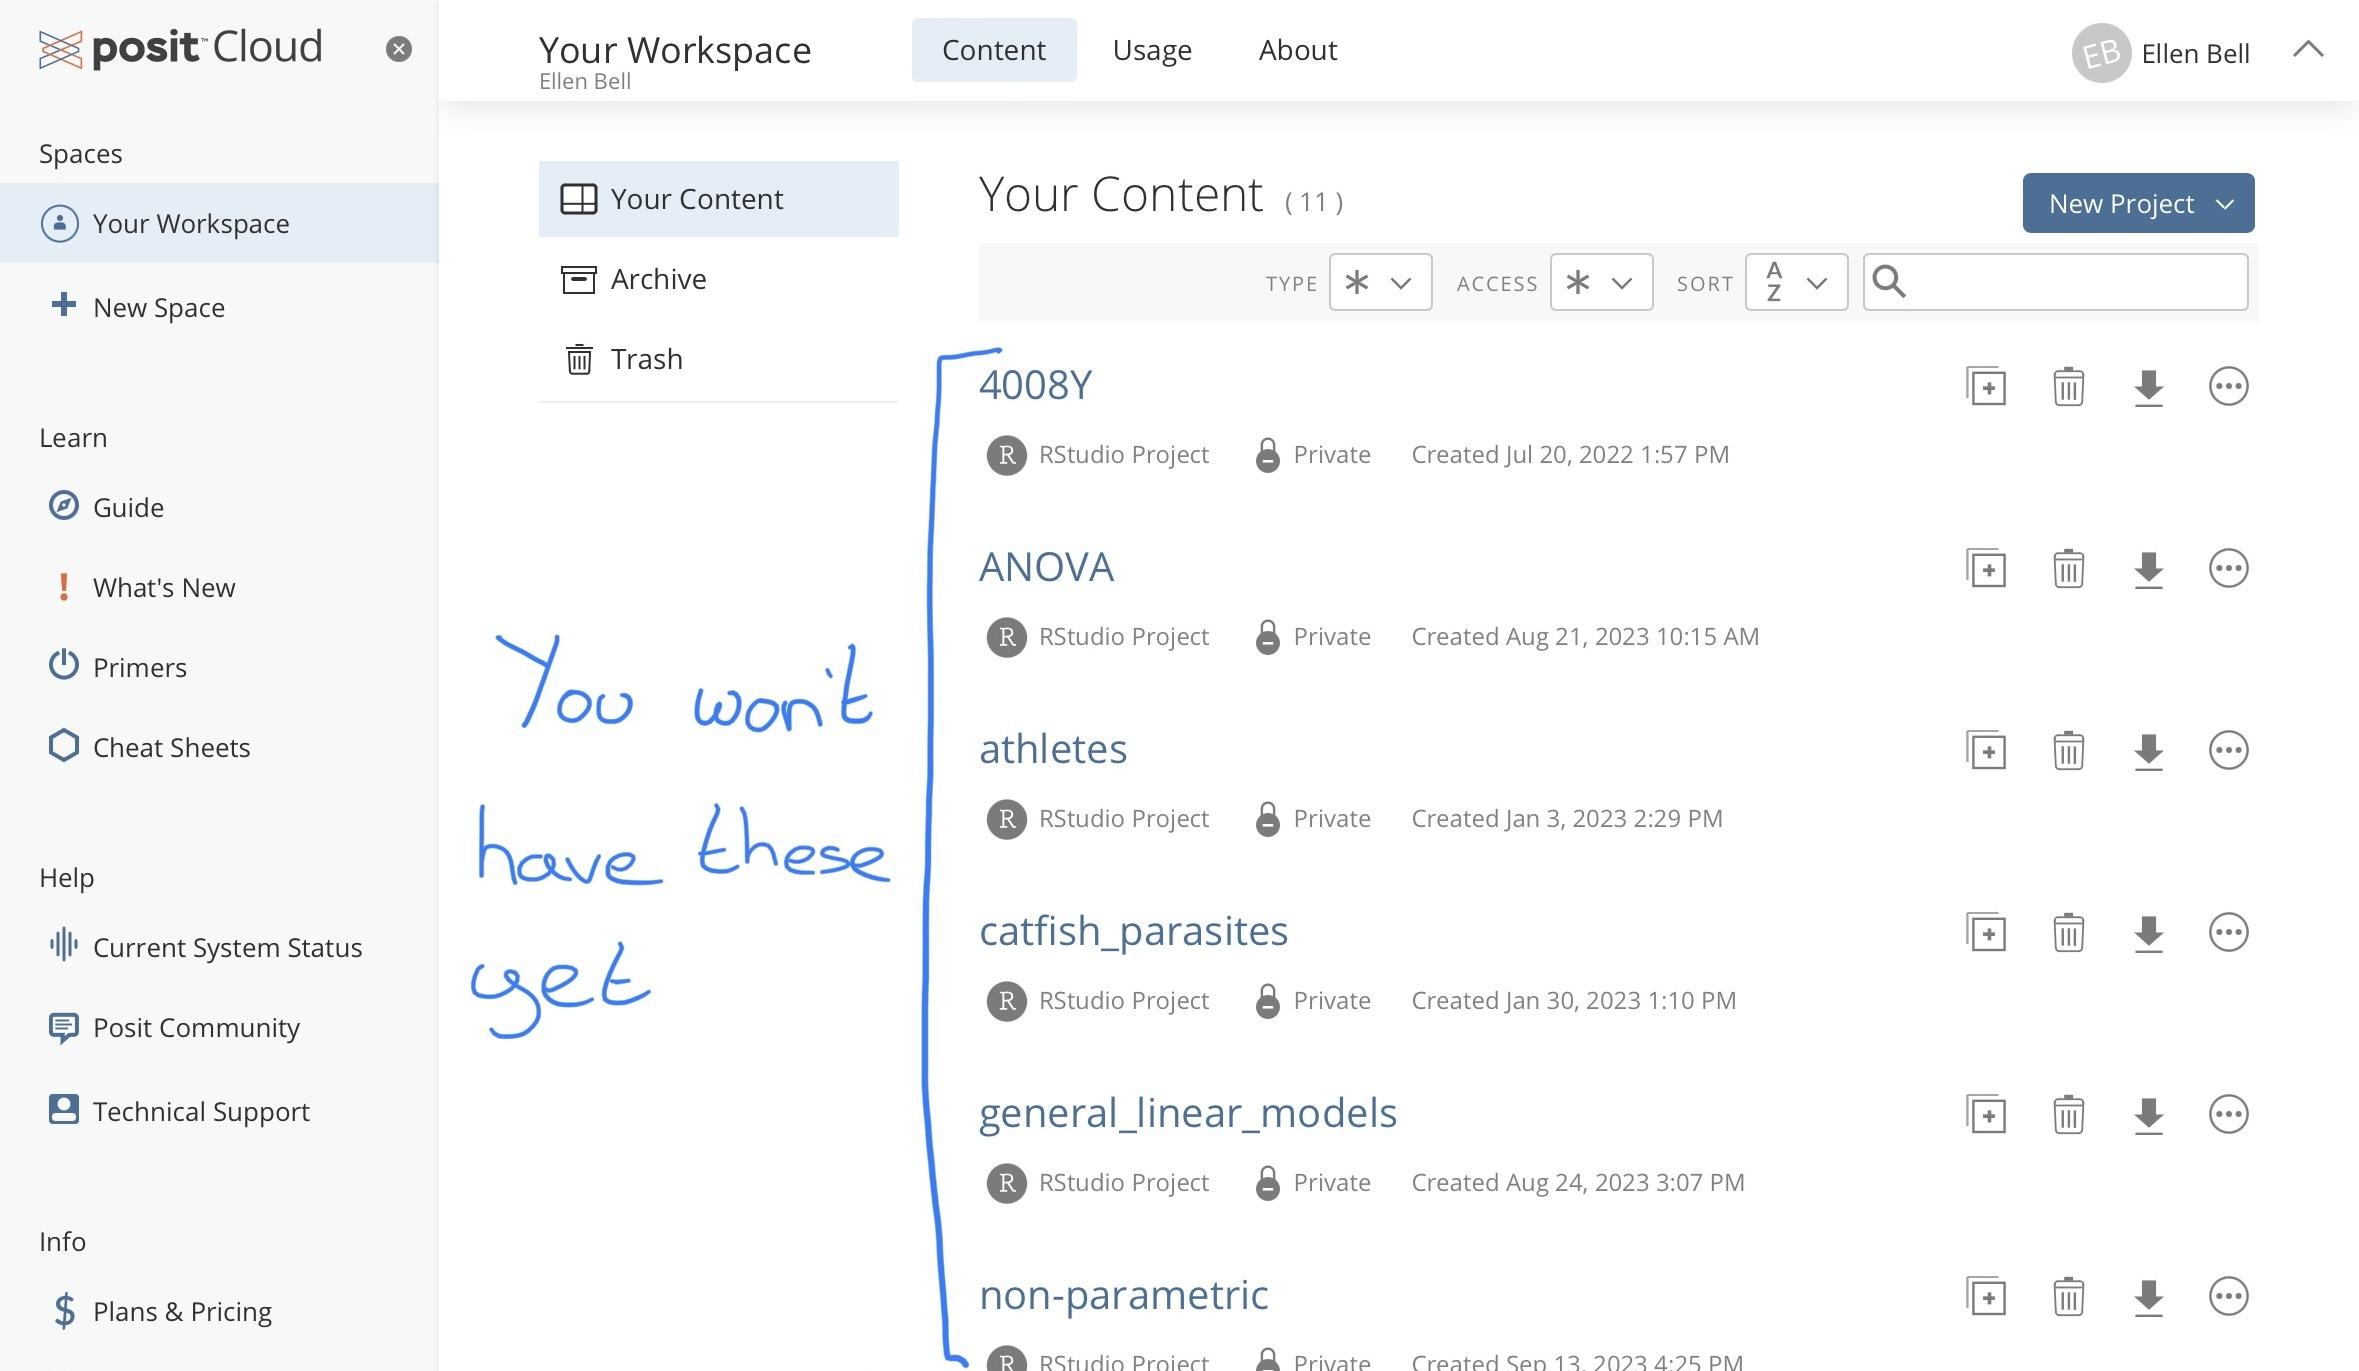
\includegraphics[width=0.9\linewidth]{figures/posit1} \caption{Your workspace in posit Cloud}\label{fig:unnamed-chunk-1}
\end{figure}

Under \textbf{Spaces} go to \textbf{Your Workspace} and under \textbf{Projects} create a \textbf{New Project \textgreater{} New R studio Project}.

\begin{figure}
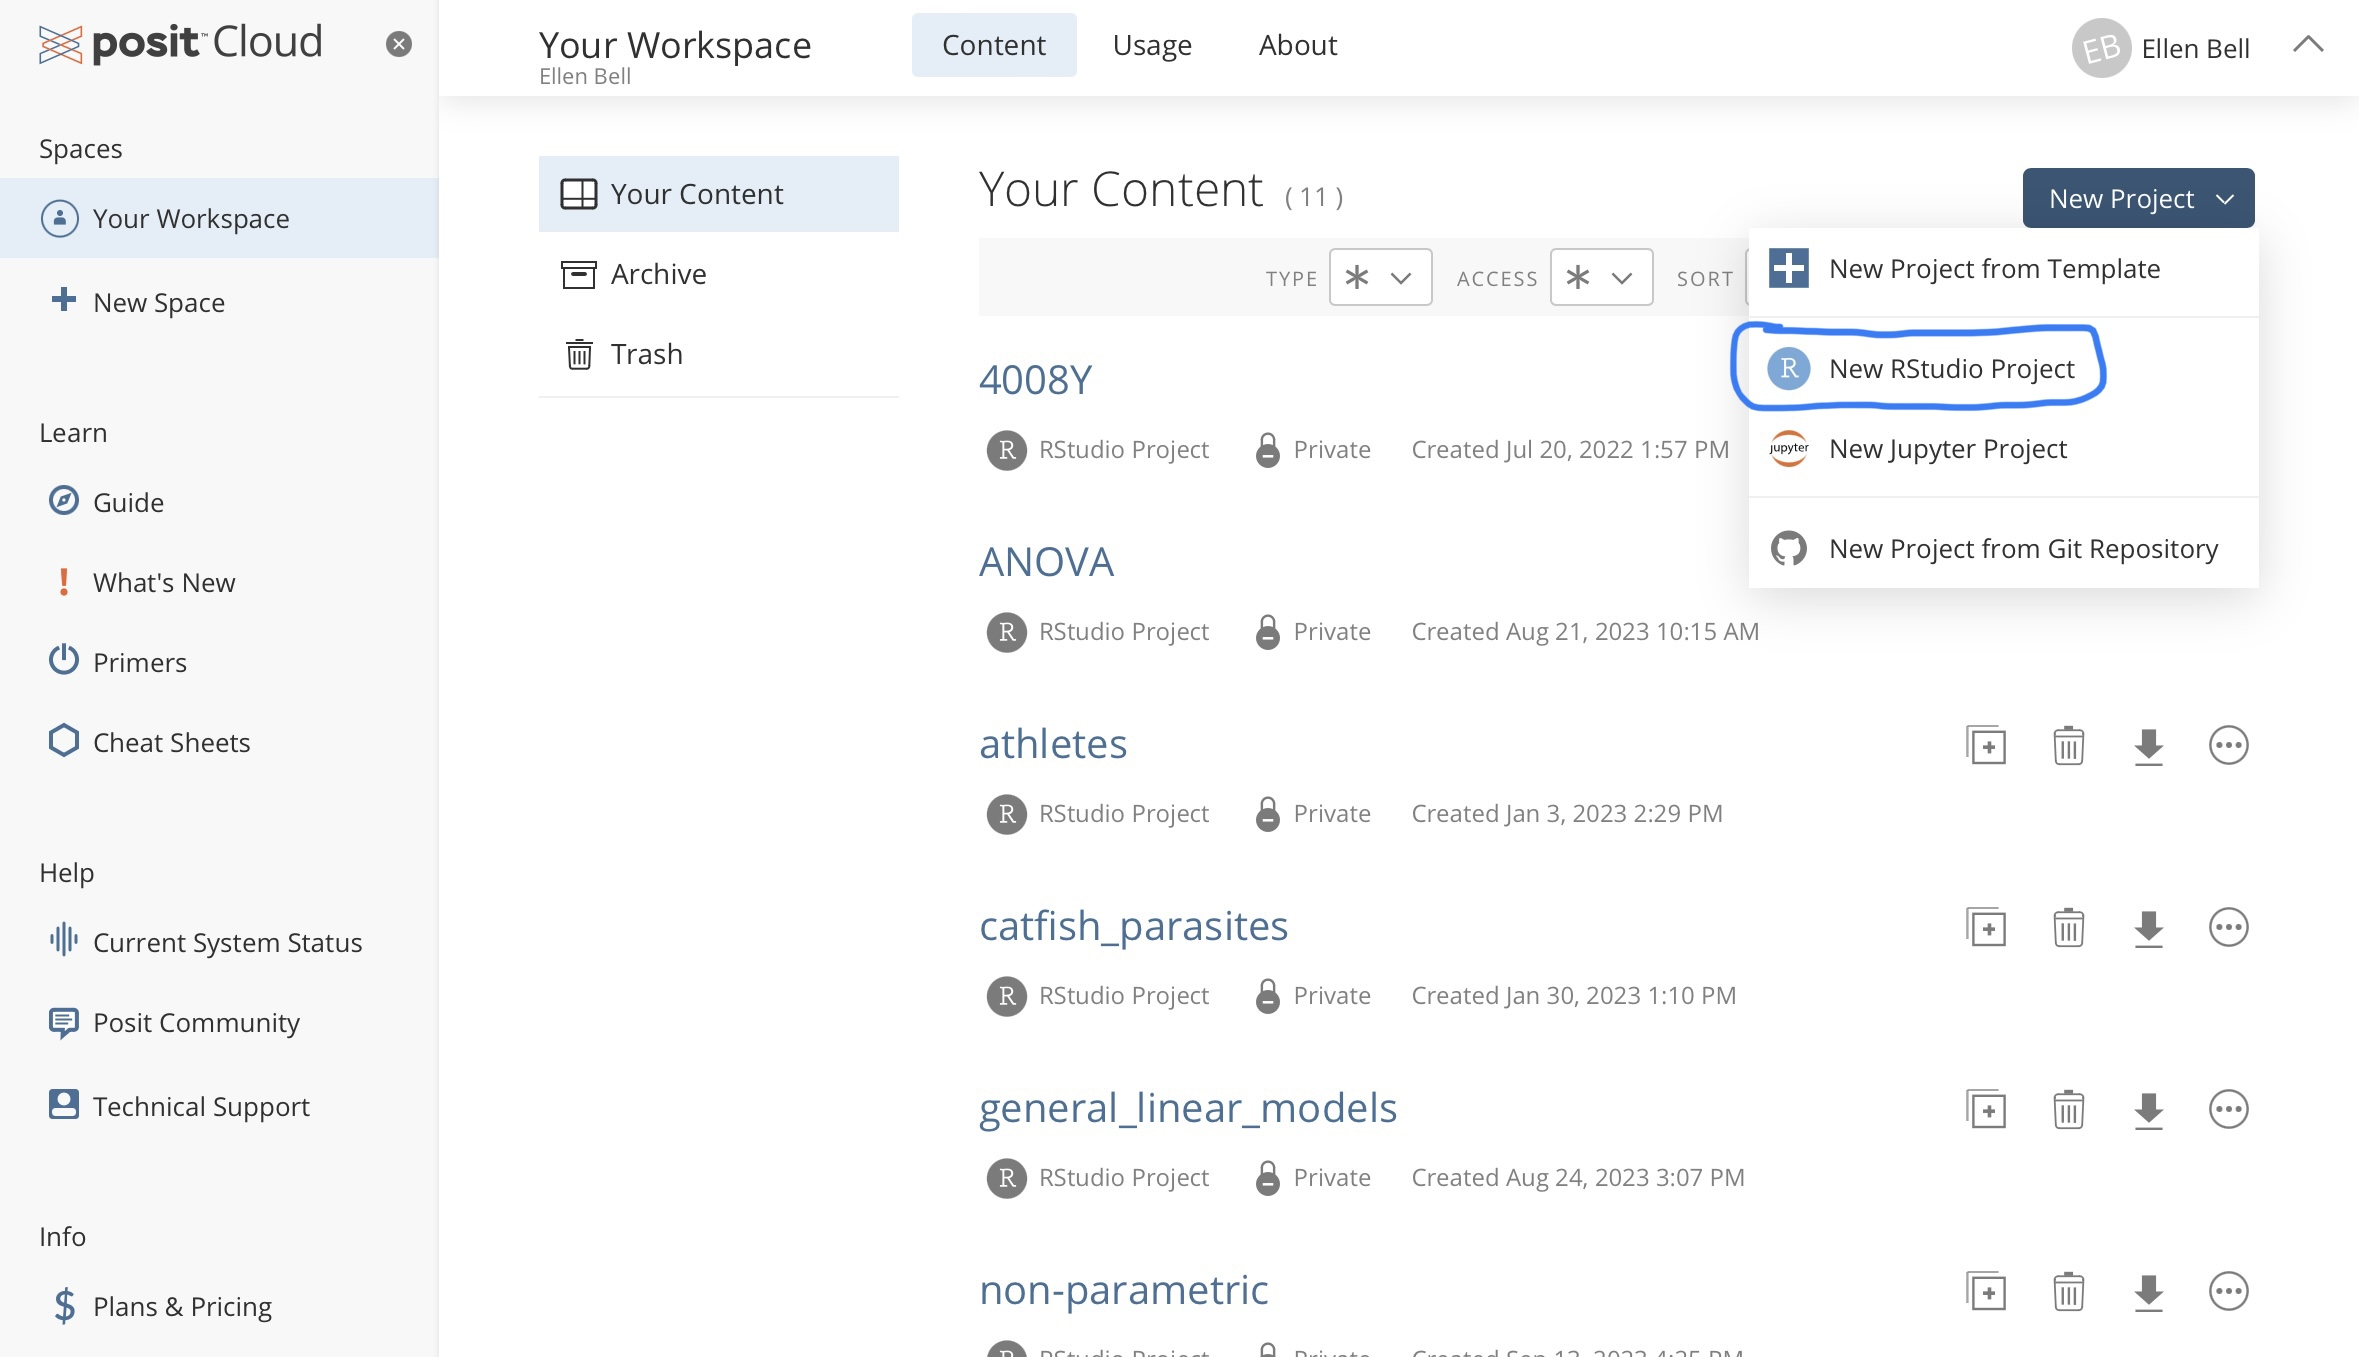
\includegraphics[width=0.9\linewidth]{figures/posit2} \caption{Creating a new project in posit Cloud}\label{fig:unnamed-chunk-2}
\end{figure}

Lets name this project \texttt{testing\_R}, notice that I have no spaces in my project name. Instead of a space I have used an underscore, there are a number of good habits you should try and adopt when project or file naming and not including spaces is one of them, we will go over this in more depth in lectures and later chapters. You can rename your project by clicking on \textbf{Untitled Project} at the top of the window, and typing in your new project name.

\begin{figure}
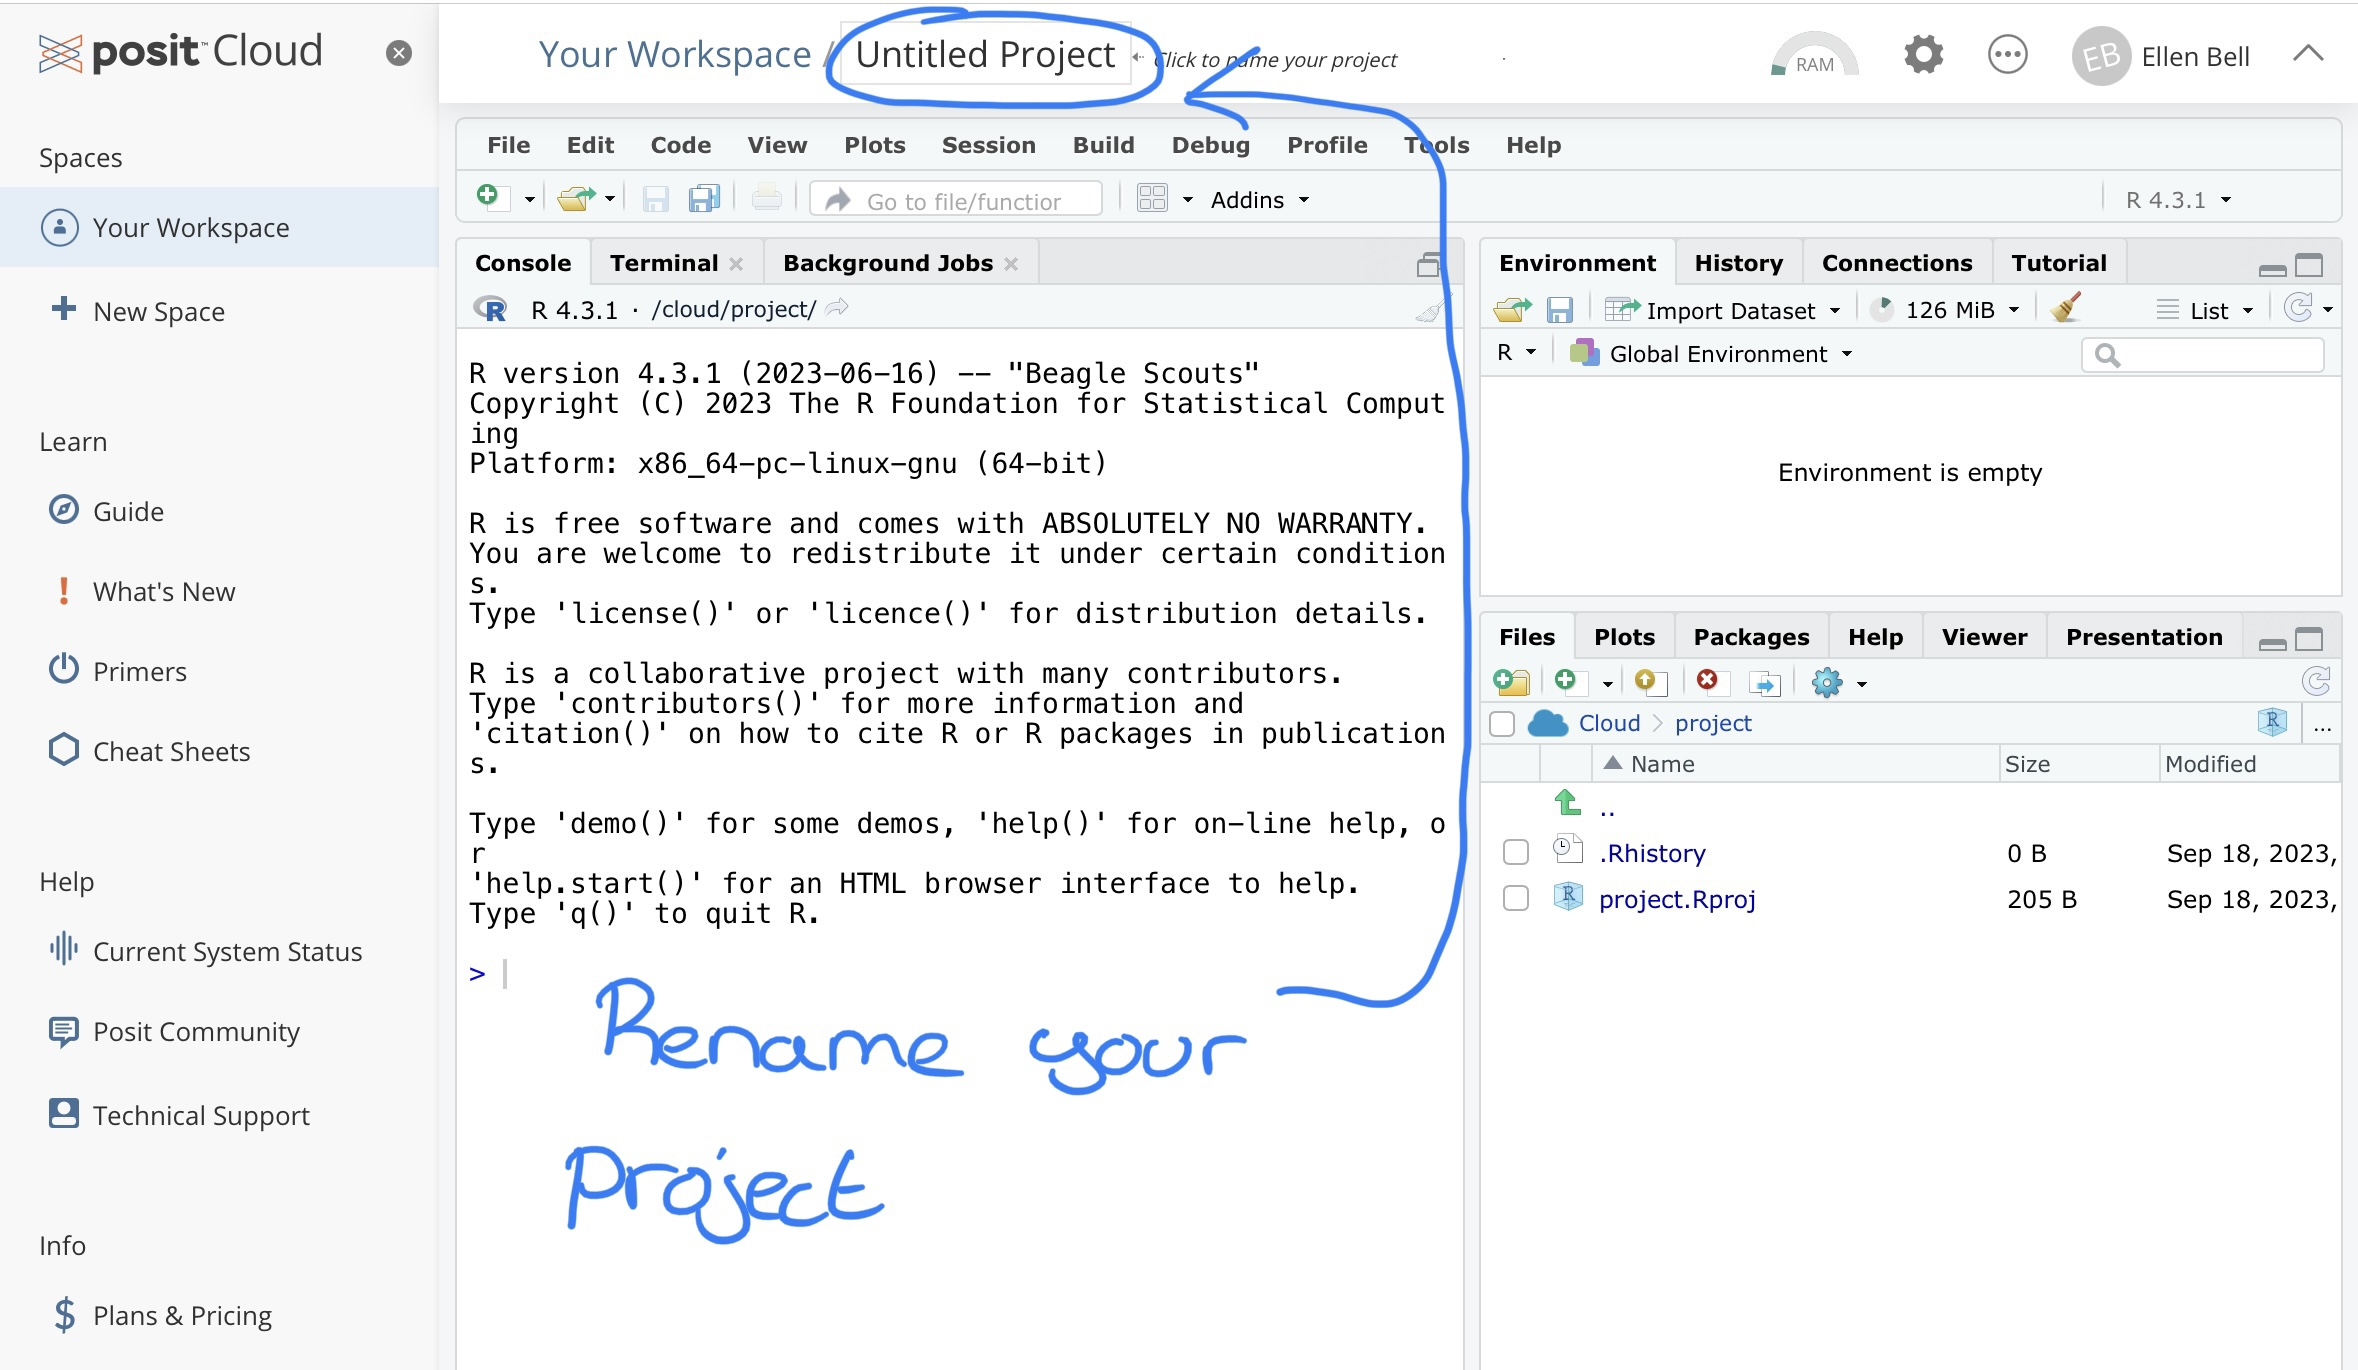
\includegraphics[width=0.9\linewidth]{figures/posit3} \caption{Renaming your project}\label{fig:unnamed-chunk-3}
\end{figure}

You will see that your new project has three panels with tabs showing the Console, Environment and Files for your project.

\begin{figure}
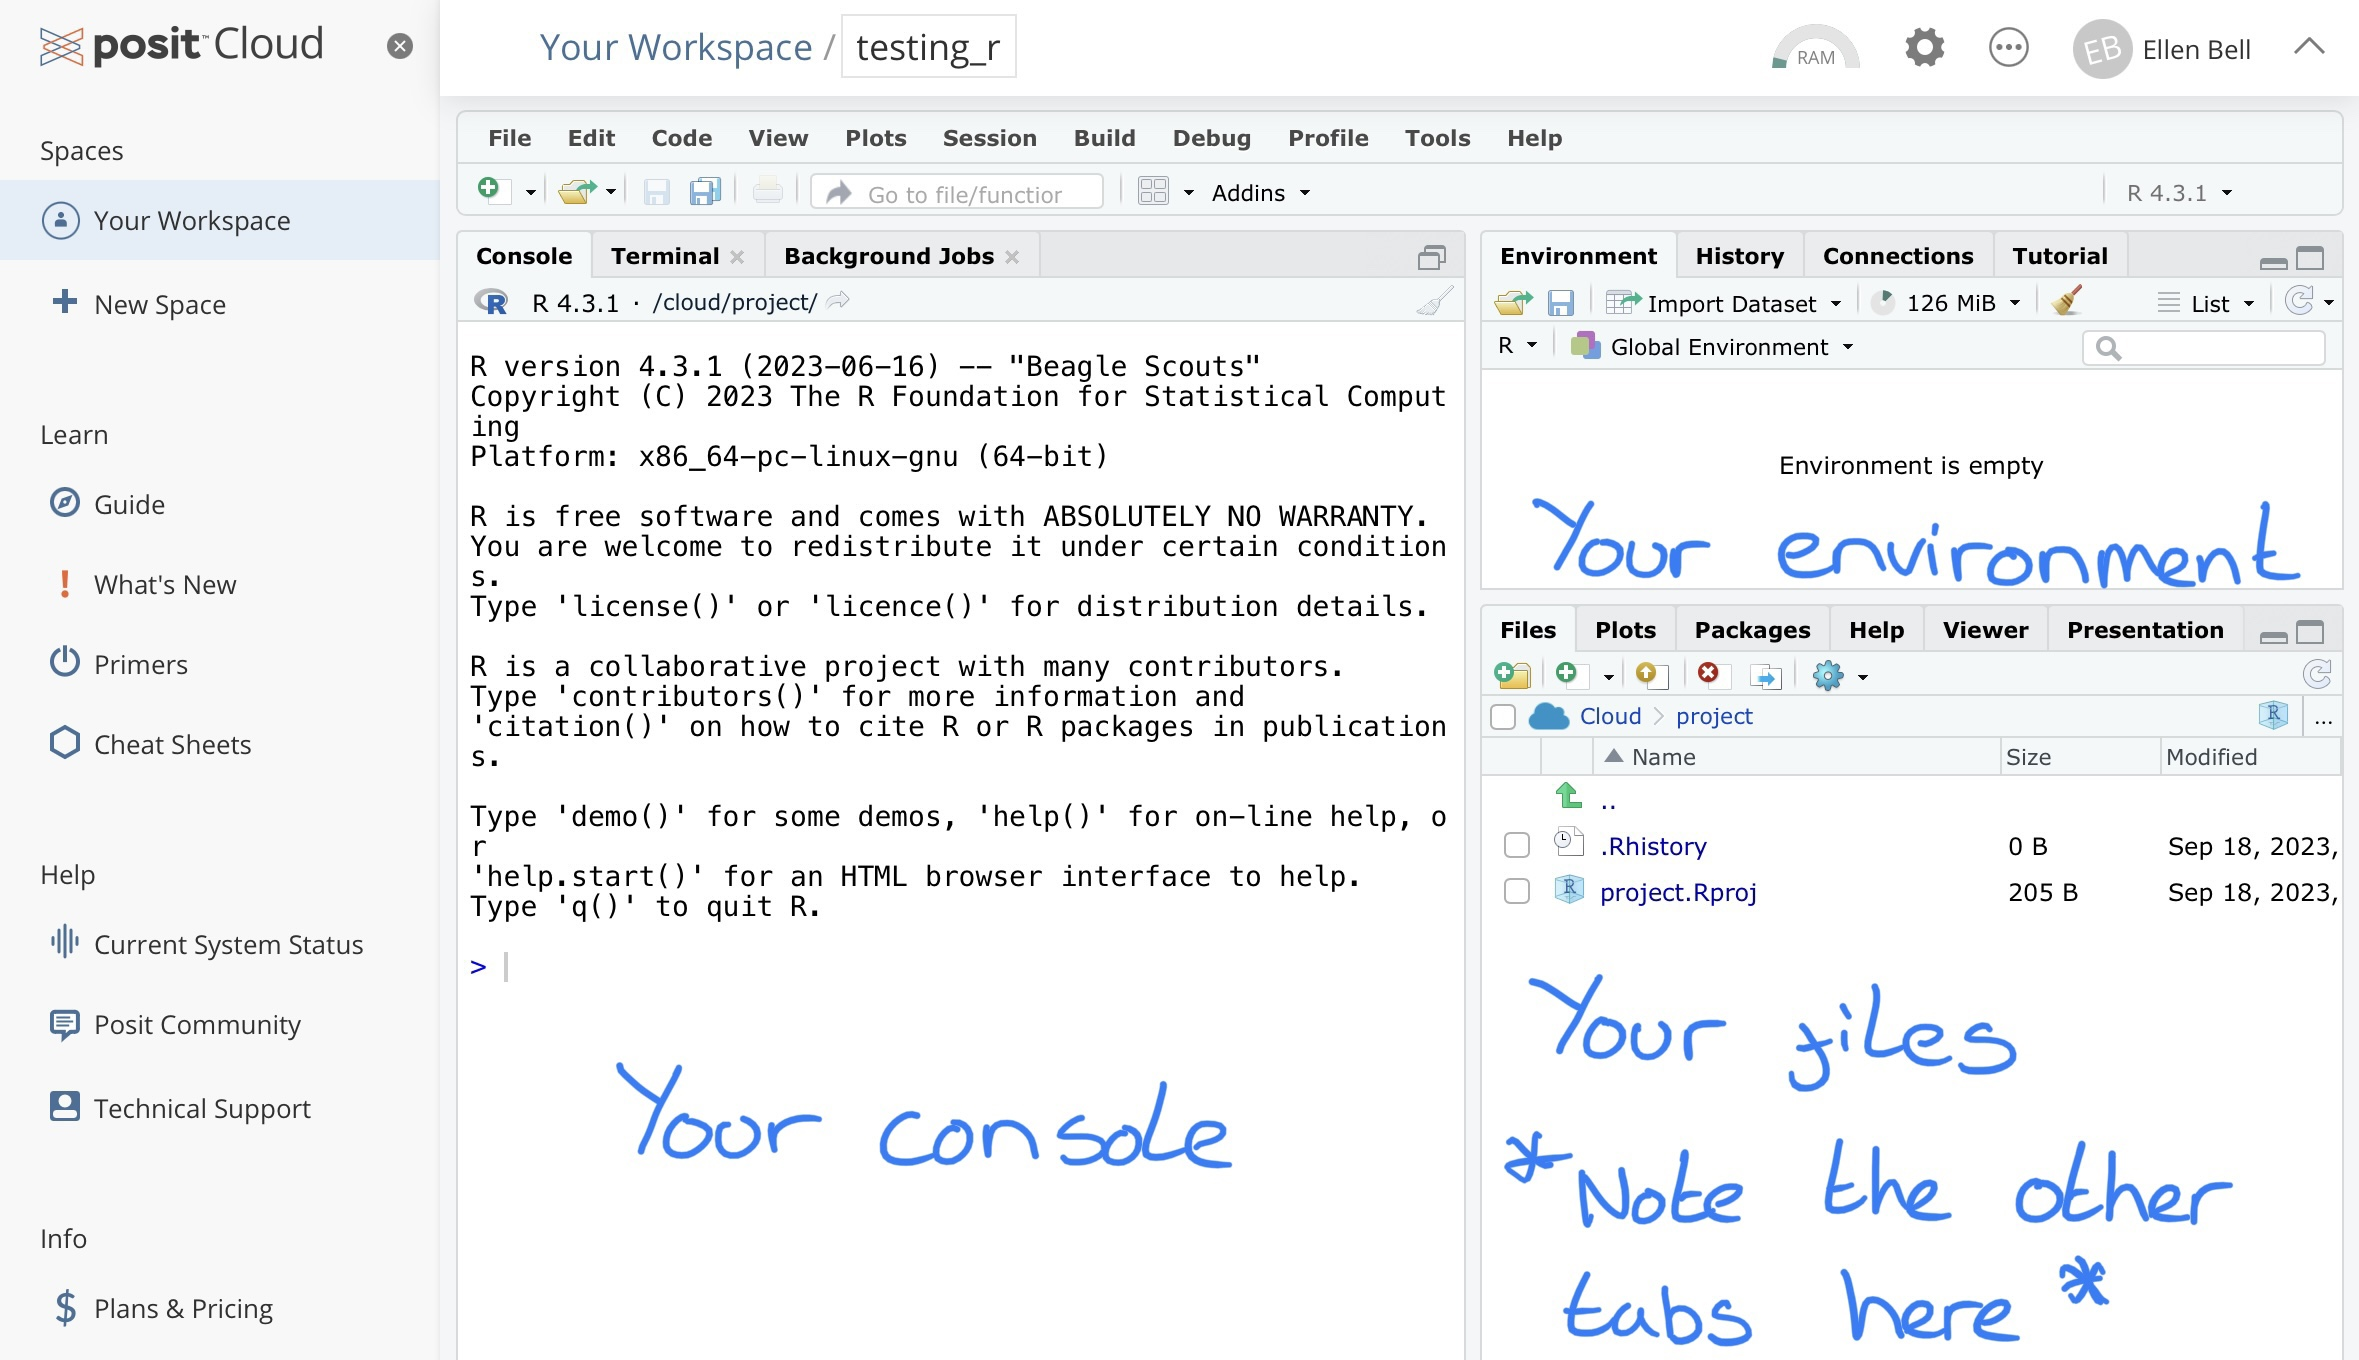
\includegraphics[width=0.9\linewidth]{figures/posit4} \caption{The three basic panels of an R Studio workspace}\label{fig:unnamed-chunk-4}
\end{figure}

\hypertarget{maximising-the-efficiency-of-your-workspace}{%
\section{Maximising the efficiency of your workspace}\label{maximising-the-efficiency-of-your-workspace}}

We know we have limited project hours on our free posit Cloud accounts to reduce your resource usage. In your project, go to settings (the cogwheel sign), Resources, and drag all of the sliders down to the minimum setting, apply the changes, this will mean the project has to restart. This will mean that running the project for 1 hour will consume 0.5 project hours. We wont be doing anything particularly computationally intensive so there is no need for RAM of CPUs to be higher.

\begin{figure}
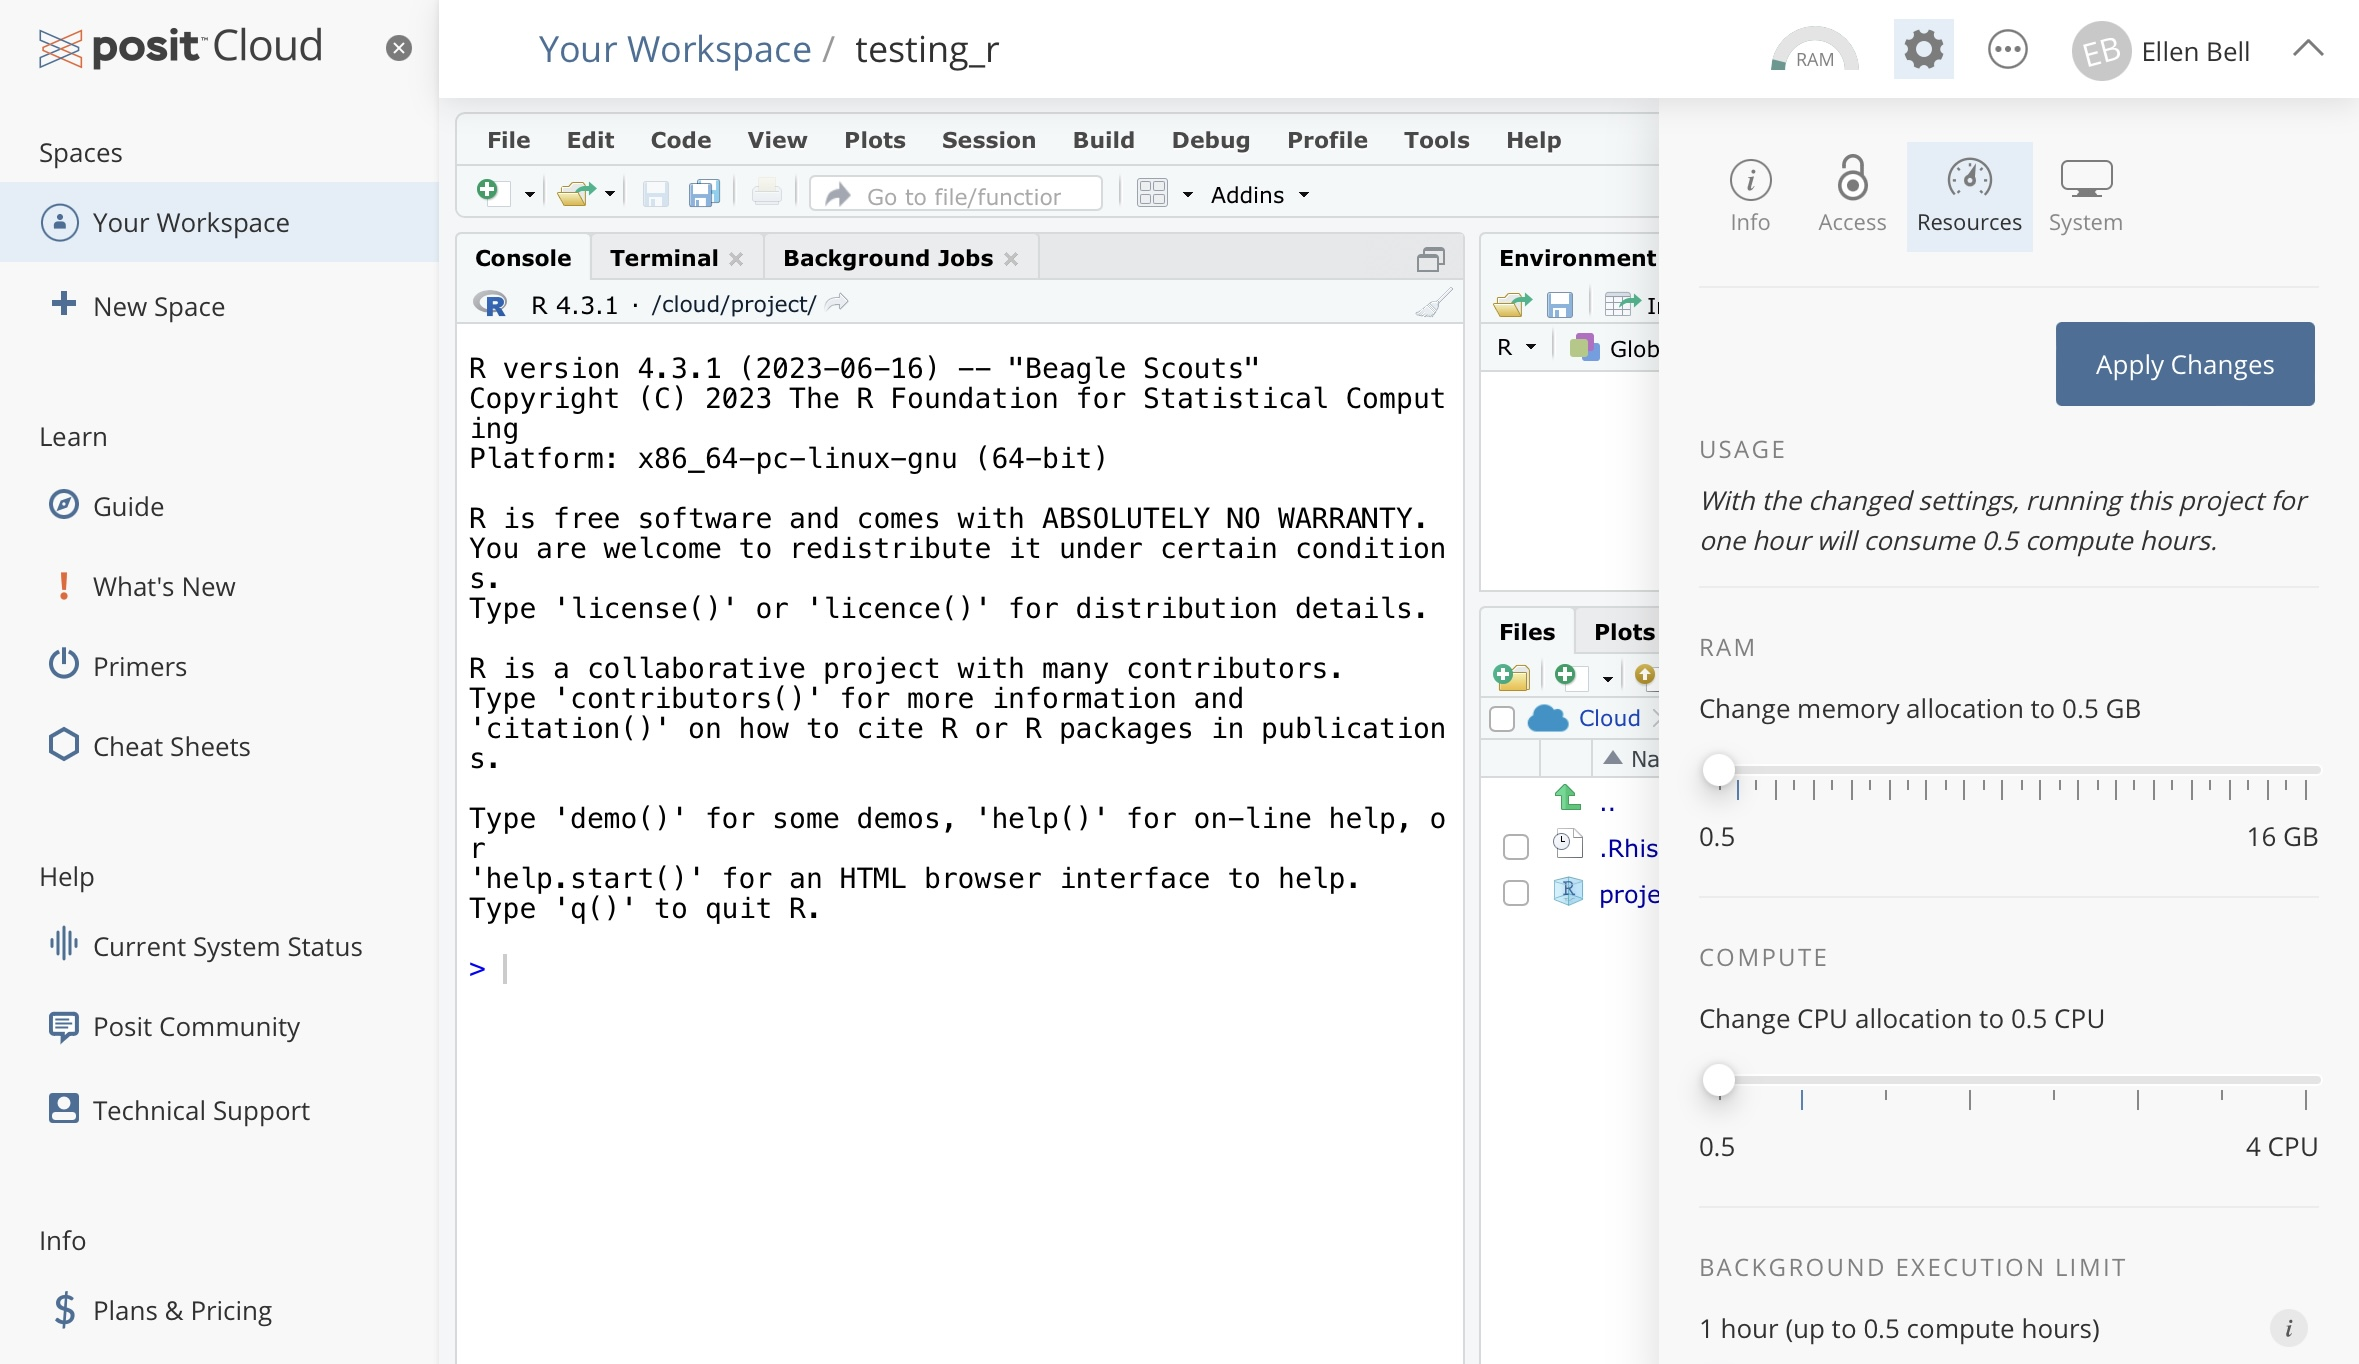
\includegraphics[width=0.9\linewidth]{figures/posit5} \caption{How to make your project more efficient}\label{fig:unnamed-chunk-5}
\end{figure}

\hypertarget{entering-commands-directly-into-the-consol}{%
\section{Entering commands directly into the consol}\label{entering-commands-directly-into-the-consol}}

Lets start by playing with some commands in the console. Type or copy and paste the simple calculation (or command) shown below, into the console. Your text should appear next to the \texttt{\textgreater{}} symbol. Press \texttt{Enter} on your keyboard, this will instruct R to run the command.

\begin{Shaded}
\begin{Highlighting}[]
\DecValTok{5} \SpecialCharTok{+} \DecValTok{9}
\end{Highlighting}
\end{Shaded}

The two final lines of your output should look like this:

\begin{verbatim}
> 5 + 9
[1] 14
\end{verbatim}

So\ldots{} your initial command \texttt{5\ +\ 9} is shown after the \texttt{\textgreater{}}, symbol and the resulting output from R is shown after \texttt{{[}1{]}}. Don't worry too much about the syntax of \texttt{\textgreater{}} and \texttt{{[}1{]}} here. You can think of \texttt{\textgreater{}} as meaning that R is ready to receive a command and \texttt{{[}1{]}} as R telling you that the answer to the first part of your question is here (in this case \texttt{14}).

Try out some other commands\ldots{} What happens when you input the following?

\begin{Shaded}
\begin{Highlighting}[]
\DecValTok{362} \SpecialCharTok{*} \DecValTok{12}
\end{Highlighting}
\end{Shaded}

\begin{Shaded}
\begin{Highlighting}[]
\DecValTok{55} \SpecialCharTok{/} \DecValTok{5}
\end{Highlighting}
\end{Shaded}

\begin{Shaded}
\begin{Highlighting}[]
\NormalTok{(}\DecValTok{40} \SpecialCharTok{/} \DecValTok{990}\NormalTok{) }\SpecialCharTok{*} \DecValTok{100}
\end{Highlighting}
\end{Shaded}

\begin{Shaded}
\begin{Highlighting}[]
\DecValTok{4}\SpecialCharTok{\^{}}\DecValTok{2}
\end{Highlighting}
\end{Shaded}

See if you can work out what 30\% of 735 is using the R console

\hypertarget{sending-commands-down-to-the-console-from-an-r-script}{%
\section{Sending commands down to the console from an R script}\label{sending-commands-down-to-the-console-from-an-r-script}}

I have already mentioned the \textbf{reproducibility} factor as an advantage of using posit Cloud. This is because you can record and run all of your commands from an R script within posit Cloud. This means that you have a written record of your analysis workflow, what you did to your data at which stage, and you can do all of this without altering the original data files! This is super important because it means that if you revisit your work in a few weeks/months/years you can see exactly what you did AND if someone else needs to rerun any of your analysis or use your workflow on some other data, they can!

So lets go about setting up your new script. You currently have three panels in posit Cloud. If you go to \textbf{file \textgreater{} New File \textgreater{} R Script} a new panel will open.

\begin{figure}
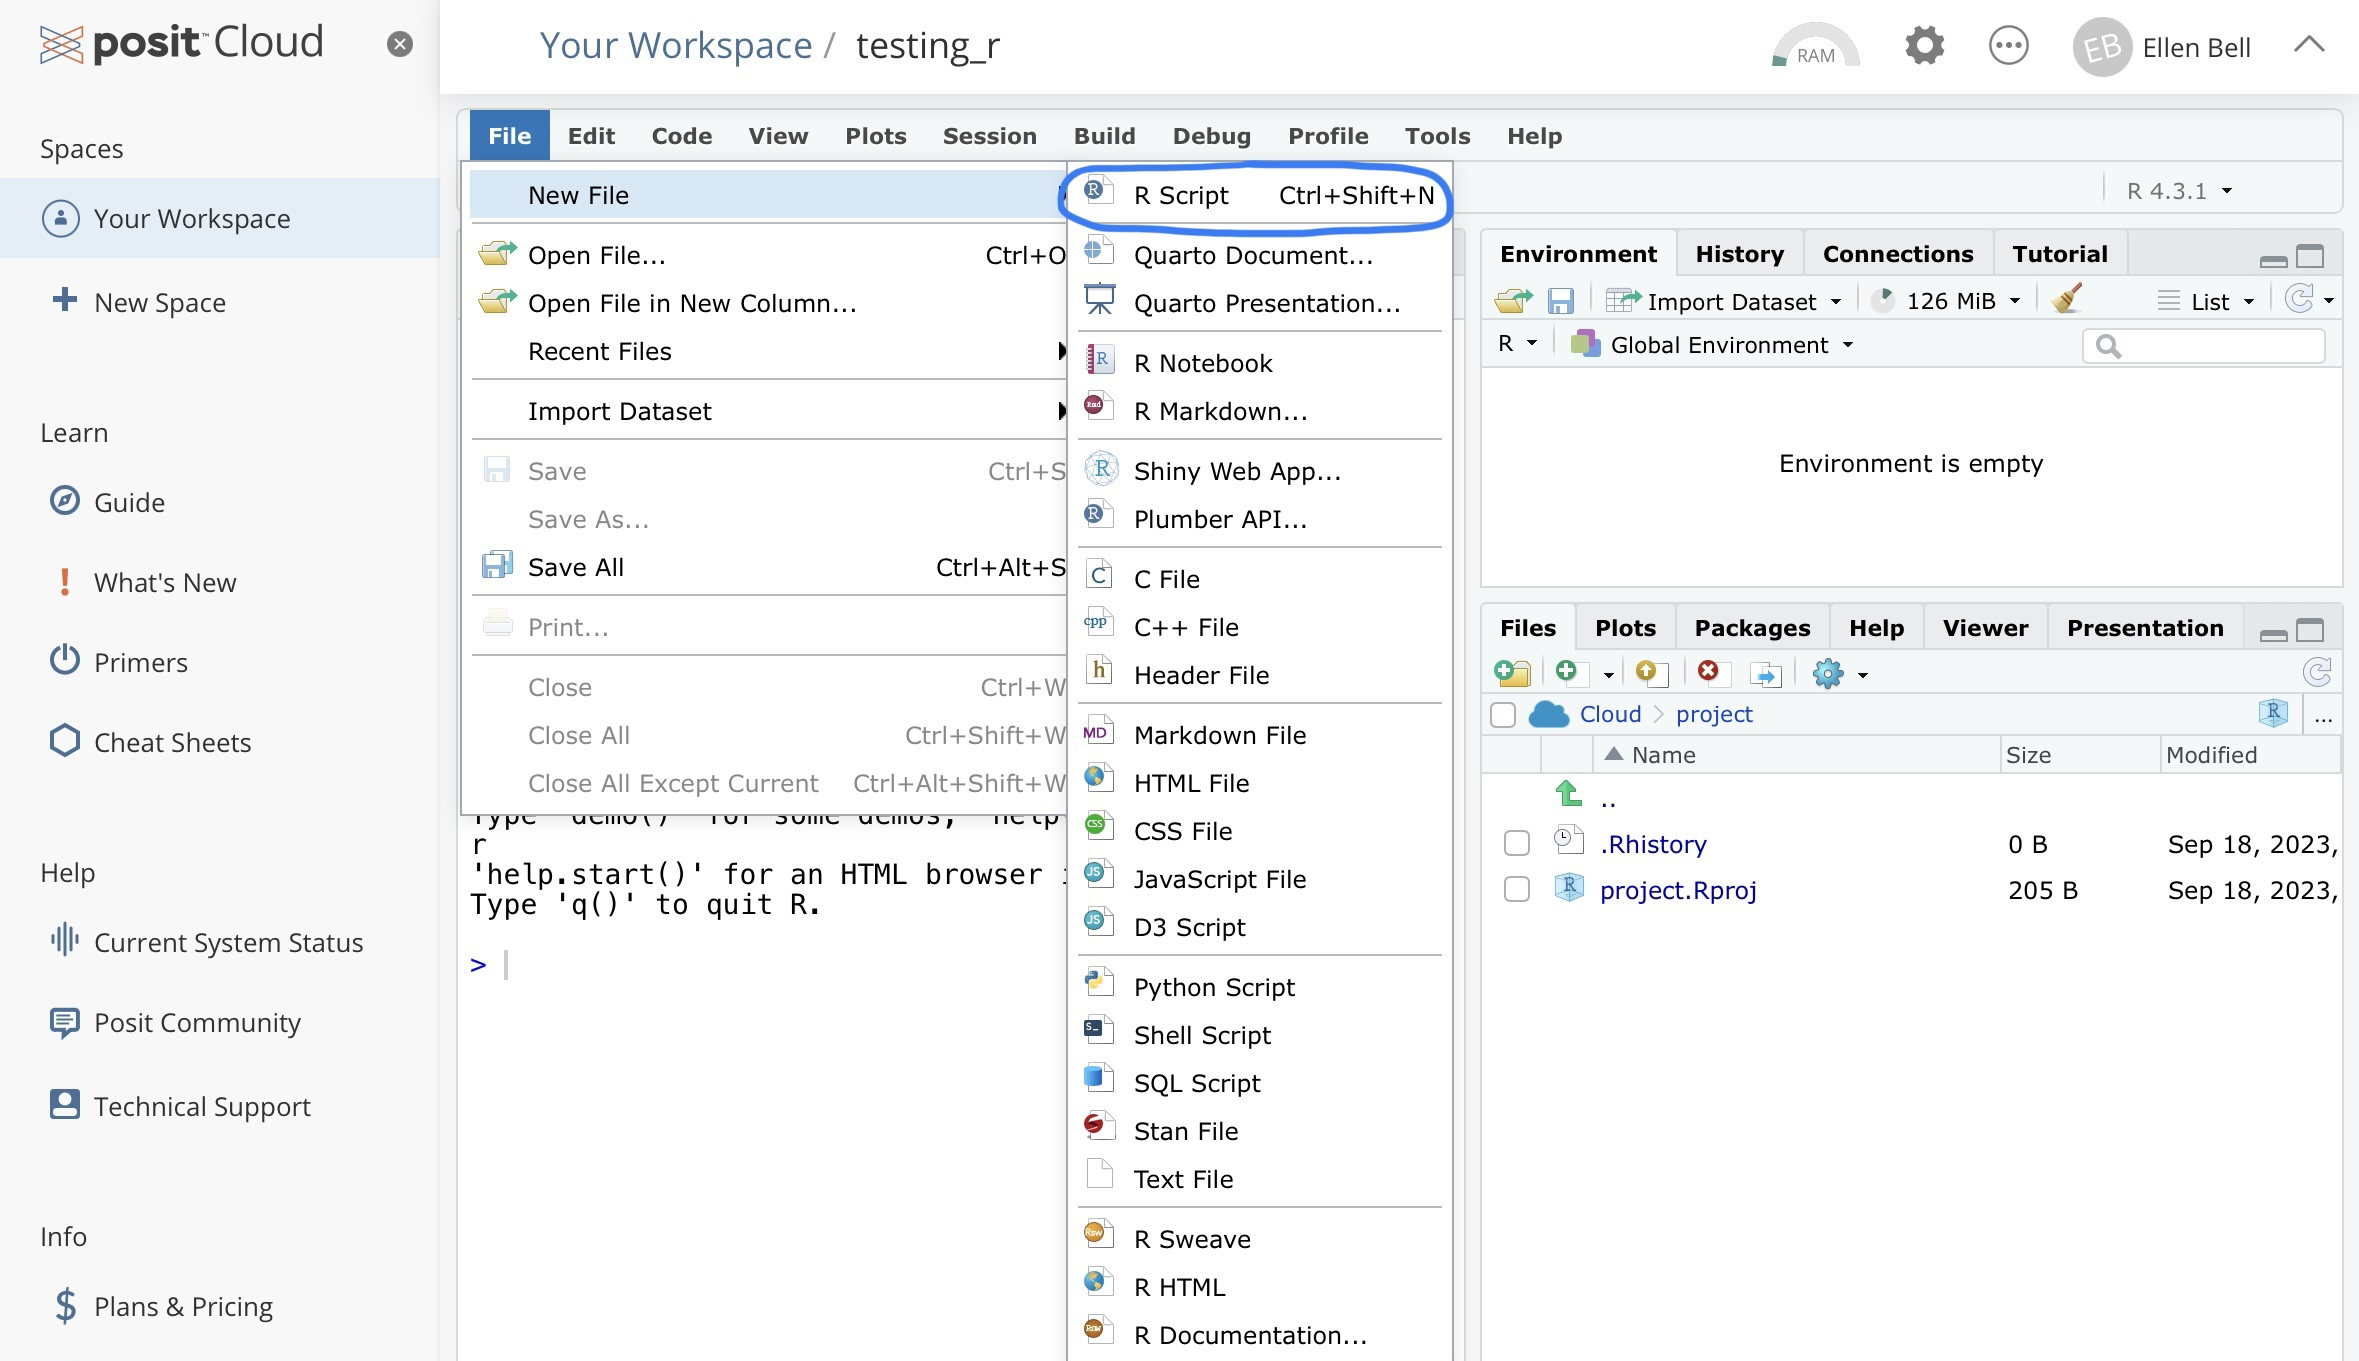
\includegraphics[width=0.9\linewidth]{figures/posit6} \caption{How to create a new R script}\label{fig:unnamed-chunk-11}
\end{figure}

\begin{figure}
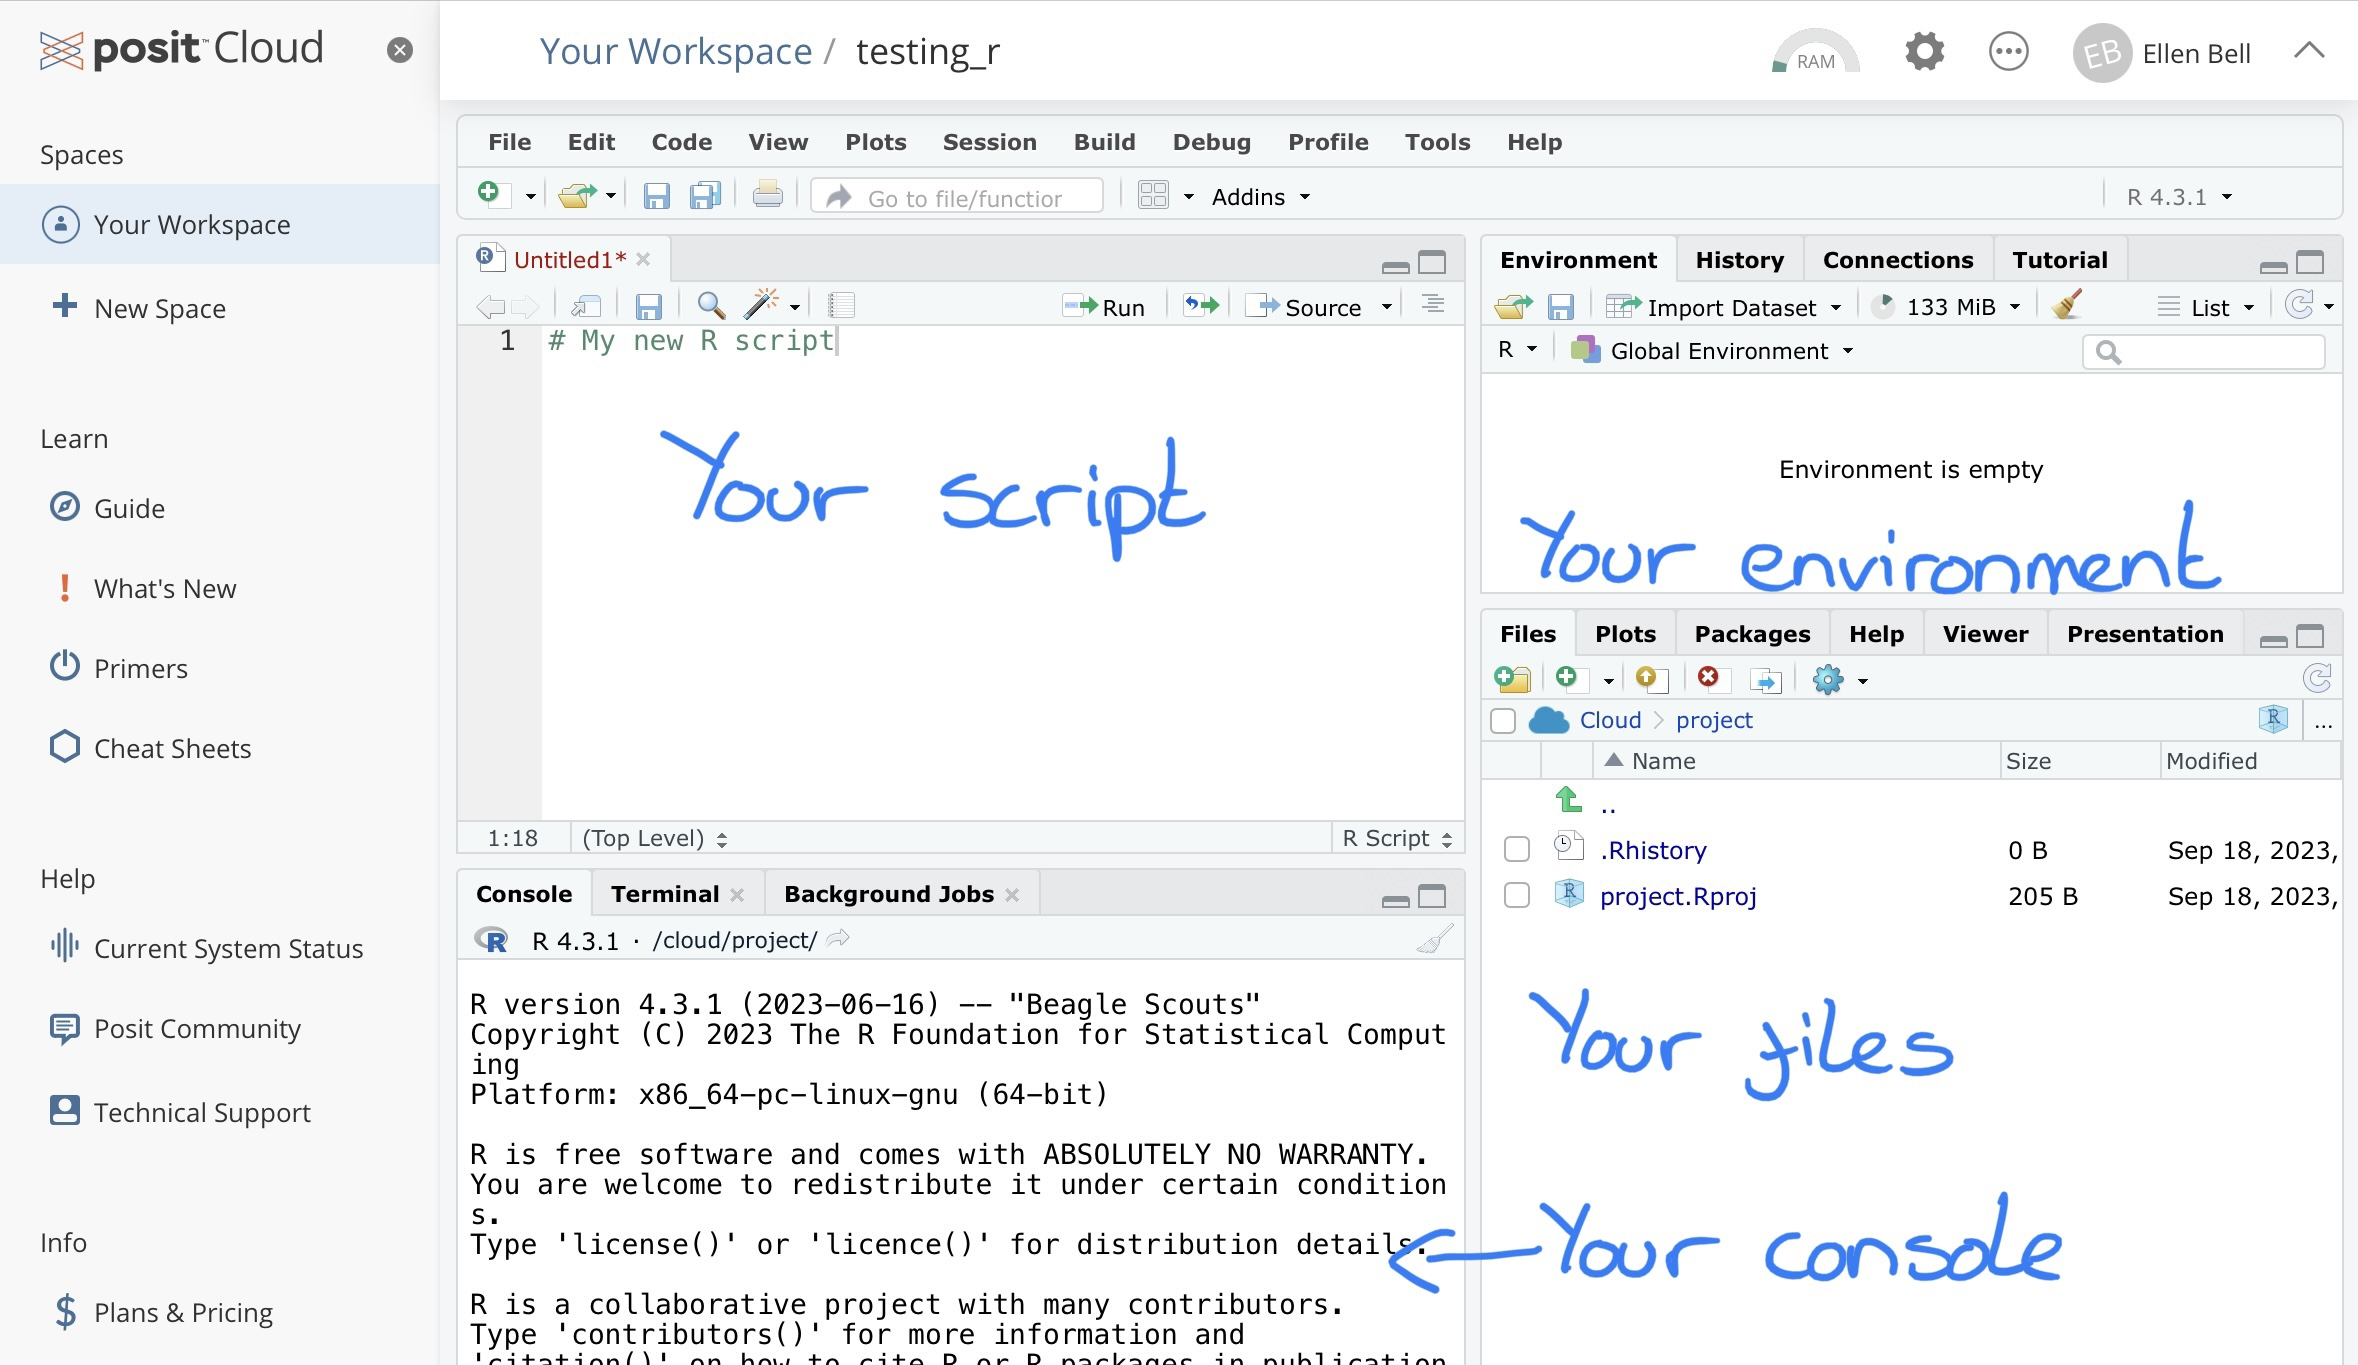
\includegraphics[width=0.9\linewidth]{figures/posit7} \caption{The four panels of an R Studio workspace}\label{fig:unnamed-chunk-12}
\end{figure}

This new panel is essentially a text file where you can write your commands into a script and then send them down to the console when you want to run them. Lets have a play. Copy the below into your new R script.

\begin{Shaded}
\begin{Highlighting}[]
\DecValTok{362} \SpecialCharTok{*} \DecValTok{12}

\DecValTok{55} \SpecialCharTok{/} \DecValTok{5}

\NormalTok{(}\DecValTok{40} \SpecialCharTok{/} \DecValTok{990}\NormalTok{) }\SpecialCharTok{*} \DecValTok{100}

\DecValTok{4}\SpecialCharTok{\^{}}\DecValTok{2}
\end{Highlighting}
\end{Shaded}

These are all commands you have run before but now if you save your script you will have a text based document with your progress saved. It doesn't make a huge amount of sense to do this now because these are just a un-associated set of calculations and we are just playing with the interface, but you could if you wanted to.

Ok, so now we are ready to execute our commands. You can do this with each calculation individually, line by line, or you can run the whole script.

To run your script line by line, place your cursor on the line you wish to run and you can either;

\begin{itemize}
\tightlist
\item
  Click on the \textbf{Run} button on the top right of the script panel
\item
  Press \textbf{ctrl + Enter} (or \textbf{Command + Enter} on mac)
\end{itemize}

Or if you wish to run the entire script you can either;

\begin{itemize}
\tightlist
\item
  Manually highlight the script and click the \textbf{Run} button or press \textbf{ctrl + Enter} (or \textbf{Command + Enter} on mac)
\item
  Press \textbf{ctrl + A} (or \textbf{Command + A} on mac) and then click the run button or press \textbf{ctrl + Enter} (or \textbf{Command + Enter} on mac)
\end{itemize}

\hypertarget{a-note-on-comments}{%
\section{A note on comments}\label{a-note-on-comments}}

When you are writing a script you can leave notes for yourself. This can be extremely useful if you need reminding on what a particular piece of script is doing. This is a good learning tool while you are still learning how to use R, but its also a good habit to get into for later. As you progress with R you will inevitably start constructing quite intricate scripts, leaving good notes on what each part of the script is doing is very useful for you and for anyone else who may later come to use your script. You can leave notes or comments in scripts if you precede them with \texttt{\#}. If R sees \texttt{\#} it will ignore all text on that line that comes after it. For example, copy and paste the following into your script and try running it line by line.

\begin{Shaded}
\begin{Highlighting}[]
\CommentTok{\# Four squared can be calculated with the following command}
\DecValTok{4}\SpecialCharTok{\^{}}\DecValTok{2}
\end{Highlighting}
\end{Shaded}

In this case I have reminded myself how to calculate 4 squared, everything after the \texttt{\#} will be ignored by R when you try to run the line.

Well Done! You have started writing and running simple code. But R is capable of doing so much more than simple calculations. Next week in Chapter 3 we will explore how we can create objects, and use packages and functions.

\hypertarget{objects-functions-and-packages---week-3a}{%
\chapter{Objects, Functions and Packages - Week 3A}\label{objects-functions-and-packages---week-3a}}

You should aim to complete this chapter in Week 3, Semester 1

\hypertarget{creating-objects}{%
\section{Creating objects}\label{creating-objects}}

As we saw in Chapter 2, R can be used to perform calculations. However, we can use R to perform tasks that are much more complex. In order to do this we are going to have to learn about objects.

Log in to your posit Cloud account and go into your \texttt{testing\_R} project. Create a new R script and save it under the name \texttt{objects}. You should see it appear as \texttt{object.R} under the \textbf{Files} tab in the bottom right panel. Run the following command using your script.

\begin{Shaded}
\begin{Highlighting}[]
\NormalTok{A }\OtherTok{\textless{}{-}} \DecValTok{50}
\end{Highlighting}
\end{Shaded}

What you have essentially done here, is told R to create an object called \texttt{A} and to store the number \texttt{50} inside it using the syntax \texttt{\textless{}-}. After running the command you should see your object \texttt{A} and \texttt{50} pop up under \textbf{Environment} and \textbf{Values} in the top right hand panel, so you can see that \texttt{50} has been stored in \texttt{A}.

Lets create some more objects

\begin{Shaded}
\begin{Highlighting}[]
\NormalTok{B }\OtherTok{\textless{}{-}} \DecValTok{6}
\end{Highlighting}
\end{Shaded}

Now see what happens if you run the following command

\begin{Shaded}
\begin{Highlighting}[]
\NormalTok{A }\SpecialCharTok{*}\NormalTok{ b}
\end{Highlighting}
\end{Shaded}

Oh dear\ldots{} we have an error\ldots{}

\begin{verbatim}
> A * b
Error: object 'b' not found
\end{verbatim}

This is because R has absolutely no flexibility with typos. It is looking for an object called \texttt{b} when there is no object called \texttt{b} in your environment. There is an object called \texttt{B}, but to R, \texttt{B} and \texttt{b} are completely different things. Try running this instead.

\begin{Shaded}
\begin{Highlighting}[]
\NormalTok{A }\SpecialCharTok{*}\NormalTok{ B}
\end{Highlighting}
\end{Shaded}

Hopefully you should now have an output that looks like this

\begin{verbatim}
> A * B
[1] 300
\end{verbatim}

This is a very simple example. But lets try to demonstrate why saving values within objects may be useful. Lets say you are interested in looking at the number of students who get freshers flu in Week 1 of teaching at UEA. You have a class size of 200 students and 15 of them report that they have contracted freshers flu. Use the following script to calculate the percentage of students with freshers flu.

\begin{Shaded}
\begin{Highlighting}[]
\CommentTok{\# Create two objects, one for your total class and one for those that have flu}
\CommentTok{\# Notice that neither of my object names contain spaces}
\CommentTok{\# If you need a space always use an underscore or full stop}
\NormalTok{total\_class }\OtherTok{\textless{}{-}} \DecValTok{200}
\NormalTok{with\_flu }\OtherTok{\textless{}{-}} \DecValTok{15}

\CommentTok{\# Calculate the percentage of students with flu in week 1}
\NormalTok{percentage\_with\_flu }\OtherTok{\textless{}{-}}\NormalTok{ (with\_flu}\SpecialCharTok{/}\NormalTok{total\_class)}\SpecialCharTok{*}\DecValTok{100}
\end{Highlighting}
\end{Shaded}

If you look in your Environment in the top right panel you should see the percentage of students with flu calculated and stored under \texttt{percentage\_with\_flu}. You can use the following command to see it printed in the console.

\begin{Shaded}
\begin{Highlighting}[]
\FunctionTok{print}\NormalTok{(percentage\_with\_flu)}
\end{Highlighting}
\end{Shaded}

Some students have been late in reporting their symptoms. A week later you hear that \texttt{7} more students also had freshers flu in Week 1. If you had been typing into the console and not using objects you would have to type this script out all over again. But you don't need to. You just need to change your entry for \texttt{with\_flu} from \texttt{15} to \texttt{22}. Do that now and re-run the script. By editing the \texttt{15}, R will overwrite the object \texttt{with\_flu} to represent the new value of \texttt{22}. If you run the last line of code then the percentage of students with flu will also update.

This may seem like a very simple example, and it is, but we are still building up your knowledge of R so you will have to take my word for it that objects will be very helpful to you as we progress :). You will also see, that objects can contain a range of different types of data. We will cover some of these in lectures, but for now lets leave objects and have a think about functions and packages.

\hypertarget{what-are-functions-and-packages}{%
\section{What are functions and packages?}\label{what-are-functions-and-packages}}

If you have the coding skills it is possible to do pretty much whatever you like with your data in R. However, why reinvent the wheel trying to write your own complex scripts, when a lot of very clever coders have already written lots of functional bits of code, known as \textbf{functions}, for general use. Functions can be thought of as a piece of code that is designed to perform a set task. R comes with lots of functions already built in, but there are also lots of additional functions that are stored in \textbf{packages}.

Packages are containers that can hold sets of functions or data and as the course progresses you will use a range of packages that contain useful functions and data. For example the data visualisation package (which you will become very familiar with later on) \texttt{ggplot2} contains ranges of functions which allow you to define how your plot or graph will look, for example \texttt{geom\_bar} is a function within the \texttt{ggplot2} package that contains the instructions required to build a bar chart.

\hypertarget{using-functions}{%
\subsection{Using functions}\label{using-functions}}

We actually have already had some exposure to functions. You used the print function earlier when you asked R to print out the value contained within the \texttt{percentage\_with\_flu} object. But lets have a go at using another function.

\begin{Shaded}
\begin{Highlighting}[]
\CommentTok{\# First of all we need some data}
\CommentTok{\# Notice the syntax, by using c() I have told R to prepare for a list of values}
\CommentTok{\# Each value is separated by a comma}
\NormalTok{data }\OtherTok{\textless{}{-}} \FunctionTok{c}\NormalTok{(}\DecValTok{2}\NormalTok{,}\DecValTok{4}\NormalTok{,}\DecValTok{6}\NormalTok{,}\DecValTok{8}\NormalTok{,}\DecValTok{10}\NormalTok{,}\DecValTok{12}\NormalTok{,}\DecValTok{14}\NormalTok{,}\DecValTok{16}\NormalTok{,}\DecValTok{18}\NormalTok{,}\DecValTok{20}\NormalTok{)}

\CommentTok{\# Now I want to know what the total value of data is if I add all the values stored within it together}
\NormalTok{total }\OtherTok{\textless{}{-}} \FunctionTok{sum}\NormalTok{(data)}
\end{Highlighting}
\end{Shaded}

In the above piece of code we have created some data, as a list of values, and stored them under the object name data. We have then used the function \texttt{sum()}. We have essentially told R that we wish it to perform the function \texttt{sum()} on everything contained within the object \texttt{data} and store it in another object called \texttt{total}. You can see the value within \texttt{total} in your environment, can you work out how to get R to print the value of \texttt{total} out?

If you ever need help working out how to use a function you can use another function \texttt{help()}. Try inputing the code below into your console.

\begin{Shaded}
\begin{Highlighting}[]
\FunctionTok{help}\NormalTok{(sum)}
\end{Highlighting}
\end{Shaded}

This should bring up a help file in your bottom right hand panel that describes and explains the use of the function \texttt{sum()}.

\hypertarget{installing-packages}{%
\section{Installing packages}\label{installing-packages}}

The \texttt{sum} function is part of the base R package that comes with any R installation. However there are lots of other useful functions that are held in additional packages. In order to use these functions, you must have the necessary packages installed in your work space. I already mentioned that we would be using a package called \texttt{ggplot2}, lets try installing and loading it in your work space.

With any package you wish to use in posit Cloud you will need to go through a two step process, first of all you need to \textbf{install} the package using the \texttt{install.packages()} function (see below for usage) and then you will need to \textbf{load} it using the \texttt{library()} function. We only need to install and load a package once per posit Cloud project but I would generally keep the commands for installing and loading packages at the top of the script I'm working on.

Try copying and running the following lines in your script;

\begin{Shaded}
\begin{Highlighting}[]
\FunctionTok{install.packages}\NormalTok{(}\StringTok{"ggplot2"}\NormalTok{) }\CommentTok{\# Install the ggplot package}
\FunctionTok{library}\NormalTok{(ggplot2) }\CommentTok{\# Load the ggplot package}
\end{Highlighting}
\end{Shaded}

Now we can try to make a simple plot using some functions from the \texttt{ggplot2} package and using an example data set called \texttt{iris} that is stored in the base R \texttt{datasets} package.

Copy the following command into your script and run it

\begin{Shaded}
\begin{Highlighting}[]
\CommentTok{\# First load the base R datasets in your workspace}
\FunctionTok{library}\NormalTok{(}\StringTok{"datasets"}\NormalTok{)}

\CommentTok{\# Then call the ggplot function and tell it that the data set you wish to use is called iris}
\CommentTok{\# We then need to tell ggplot how to map our variables}
\CommentTok{\# The aes function is an aesthetic tool that allows us to define variables for the x and y axes}
\CommentTok{\# We then use the geom\_point function to instruct R to built a scatter plot}
\CommentTok{\# A second use of the aes function tells R to color points by species}
\FunctionTok{ggplot}\NormalTok{(}\AttributeTok{data =}\NormalTok{ iris,}\FunctionTok{aes}\NormalTok{(}\AttributeTok{x =}\NormalTok{ Sepal.Length, }\AttributeTok{y =}\NormalTok{ Sepal.Width)) }\SpecialCharTok{+} 
  \FunctionTok{geom\_point}\NormalTok{(}\FunctionTok{aes}\NormalTok{(}\AttributeTok{colour=}\NormalTok{Species)) }
\end{Highlighting}
\end{Shaded}

Those sharped eyed among you may have noticed that the short script defining our plot goes over two lines and contains a \texttt{+} and an indentation on the second line. The \texttt{+} and indentation is essentially allowing you to pipe one line of code into the next. This allows you to add more detailed instructions on how you would like your graph to be built and linking together multiple functions. Don't worry if this is a lot to take in at this stage, as we progress with \texttt{ggplot2} we will revisit this in more detail.

\hypertarget{what-do-i-do-if-i-get-an-error-message}{%
\section{What do I do if I get an error message?}\label{what-do-i-do-if-i-get-an-error-message}}

Error messages are almost guaranteed when working regularly with R, they are super common, don't panic when you eventually run into one. In fact you may remember that we already encountered one earlier in this chapter, that particular error was caused by a typo. Generally the most common causes of error messages are;

\begin{itemize}
\tightlist
\item
  A typo (you can reduce risk of this by consistently labeling your files and objects)
\item
  A mistake in syntax (missing or un-closed; \texttt{()}, \texttt{""}, or missing \texttt{,})
\item
  Missing dependencies (maybe you didnt install or load a package correctly, or maybe if your running a longer script, you are trying to call an object that you haven't created yet)
\end{itemize}

This is by no means an exhaustive list but when I run into errors its normally because of one of the above. The trick is don't panic and read the error message carefully, it often tells you what is wrong. Then look over your script slowly to troubleshoot. And if you are genuinely stuck and the error doesn't make sense, run it through Google, I can almost guarantee you wont have been the first person to have that error message.

Well done everyone. I hope you have enjoyed this weeks session. Next week is our first workshop and we will start to use some of these new found skills in tandem and start to look at using them on some new data.

\hypertarget{references}{%
\section{References}\label{references}}

Wickham, Hadley, Winston Chang, Lionel Henry, Thomas Lin Pedersen, Kohske Takahashi, Claus Wilke, Kara Woo, Hiroaki Yutani, and Dewey Dunnington. 2021. Ggplot2: Create Elegant Data Visualisations Using the Grammar of Graphics. \url{https://CRAN.R-project.org/package=ggplot2}.

\hypertarget{data-frames}{%
\chapter{Directories and data frames - Week 4A - Workshop 1}\label{data-frames}}

This week we don't have any lectures but we do have an in person workshop. The section to complete this week may be a little more chunky than usual, complete what you can during the workshop and then finish it off in your own time. Do make use of the demonstrators if any of the exercises so far haven't made sense.

\hypertarget{data-entry}{%
\section{Data Entry}\label{data-entry}}

Let's have a look at some actual data now, Figure 4.1 shows some lab notes taken during the data collection phase of a small research project to investigate parasite load in 2 small populations of the flour beetle \emph{Tribolium castaneum}. Each beetle has an ID, a measure of wing casing in mm (which is a good proxy for overall size) and a tally for the number of tapeworm cysticercoids dissected out. In terms of data handling and analysis, we need this data to be stored digitally and we need to have it ordered sensibly in a spreadsheet. We covered what to look for in a tidy, well ordered spreadsheet in our week 3 lecture. Have a go at entering the data from Figure 4.1 into an Excel spreadsheet. When you're done go to \textbf{File \textgreater{} Save As\ldots{}}, name your spreadsheet something sensible and make sure you select a sensible place to save it to, where it says \textbf{File Format:} select \textbf{Comma-separated Values (.csv)}.

\begin{figure}
\includegraphics[width=0.9\linewidth]{figures/parasite_burden} \caption{Lab notes for wing case size (mm) and parasite burden of 20 *Tribolium castanium*}\label{fig:unnamed-chunk-25}
\end{figure}

\hypertarget{a-note-on-naming}{%
\subsection{A note on naming}\label{a-note-on-naming}}

While we are on the subject of naming, I am going to take a moment to go over a few good rules to follow. You have just created names for some variables and for a file. You will also frequently have to name folders/directories and objects while working in R, so naming is something that you are repeatedly going to have to do. It therefore makes sense for you to learn how to do it well.

\begin{itemize}
\item
  Keep names meaningful - Over the course of your degree you will create a lot of files and folders/directories. You will also frequently be naming data variables and objects. You need to be able to easily recognise what is what so informative names are better then arbitrary names. So \texttt{girraffe}, \texttt{elephant}, \texttt{hippo} are better names then \texttt{1}, \texttt{2} and \texttt{3}.
\item
  Make versions obvious - There will be occasions when you want to save new information in a file or object but keep the original untouched. You may be experimenting or you may want the option to revisit to your original work. In these instances it makes sense to save your edits to a new version of the original file or object. If you do this and especially if you are sharing it with others make it clear. I tend to add my initials and a version identifier (e.g.~eb\_v1, eb\_v2) as a suffix to the file name.
\item
  Keep names short - Typing takes time, its boring, and the more you type the greater the risk of a typo. So keep names short. So \texttt{trunk\_length} is better than \texttt{elephant\_trunk\_length\_cm}, there is important information in the second name but you can store this as a comment or a note.
\item
  Avoid spaces - Lots of software packages hate spaces, including R. If you can get out of the habbit of using spaces and instead use \texttt{\_} your future self will thank you.
\item
  Abide by the rules for R - R does have some rules of its own for naming. Names must \textbf{not} start with a number, but numbers may be used provided the first character is a letter. You can also use \texttt{.} or \texttt{\_}, but avoid spaces at all costs. You may use upper or lower case letters, but remember R is case sensitive so will see \texttt{Elephant} and \texttt{elephant} as different. I try to keep to a lower case and use \texttt{\_} instead of spaces, it keeps everything uniform and saves me time (this style is known as snake\_case).
\end{itemize}

Now go back to your spreadsheet, do your variables and file names follow a sensible naming convention?

\textbf{Make sure you have a demonstrator check your work before moving onto the next step.}

\hypertarget{workspace}{%
\section{Setting up your R workspace}\label{workspace}}

This is a new piece of analysis, we will be carrying forward principals from the previous chapters but scripts and data will be new. So its a good idea to start with a fresh clean workspace. So lets set up a new project in posit Cloud, follow the steps from Chapter 2 if you cant remember how to do this and name this project \texttt{tribolium\_parasites}. Its always good to keep a well organised tidy workspace, generally I will start a new project in posit Cloud if I am working on a new series of questions with a new data set or sets.

For this project you need to make sure two packages are installed. Copy the following directly into your console.

\begin{Shaded}
\begin{Highlighting}[]
\FunctionTok{install.packages}\NormalTok{(}\StringTok{"tidyverse"}\NormalTok{)}
\FunctionTok{install.packages}\NormalTok{(}\StringTok{"janitor"}\NormalTok{)}
\end{Highlighting}
\end{Shaded}

We will be moving towards doing some more comprehensive data handling so setting up your workspace is going to become more and more important. If you can get into the habit of setting up your workspace properly at the start of each project you will thank yourself later. A well developed project will contain several files including;

\begin{itemize}
\tightlist
\item
  Input data
\item
  Scripts
\item
  Outputs
\end{itemize}

Under \textbf{Files} in the bottom right panel create a \textbf{New Folder}, for each of the following;

\begin{itemize}
\tightlist
\item
  data
\item
  scripts
\item
  figures
\end{itemize}

\textbf{Make sure you copy the names over exactly, or some of the commands that we will be using later wont work}

A tidy workspace will help you find the things you need when you need them and will reduce the risk of loosing things.

\hypertarget{a-note-on-directories-and-their-structure}{%
\subsection{A note on directories and their structure}\label{a-note-on-directories-and-their-structure}}

Working with text based interfaces like R, where you are writing and running commands, means that we need to have some understanding of the underlying computer architecture. You need to have some appreciation for how files are organised within folders/directories and why its important to know which directory you are working from with R.

Under \textbf{Files} in the bottom right panel of your screen you will see a file with the ending .Rproj. This is an R project file which tells R where you are working in the server. It means that R will automatically treat your project location as the \textbf{working directory}. If you wish to access files in any of the folders you have just created you will need to tell R the \textbf{path} that it needs to follow in order to access these files. There are two types of path;

\begin{itemize}
\tightlist
\item
  \textbf{absolute} paths, which refer to the same location in a file system relative to the root directory (don't worry if that doesn't make too much sense at this stage). For example, in Figure 4.2, if you wanted to access files in the \texttt{/work} directory but were already in any of the other directories like \texttt{/dev}, an absolute path would work from wherever you were working this would be \texttt{/home/jono/work}.
\item
  \textbf{relative} paths, which refer to a location in the file system relative to the directory you are currently working in. For example, in Figure 4.2, if you were working in the \texttt{/home} directory and wanted to access files in \texttt{/work} a relative path would look like \texttt{jono/work}. This is fine from the \texttt{/home} directory, but the path would not work if you were working in, for example \texttt{/lib}.
\end{itemize}

\begin{figure}
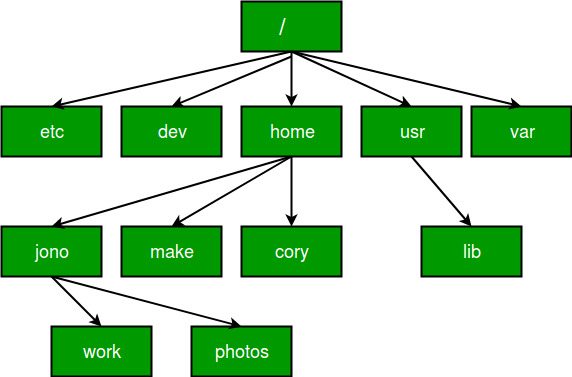
\includegraphics[width=0.9\linewidth]{figures/absolutePathNames} \caption{Absolute vs Relative Paths}\label{fig:unnamed-chunk-27}
\end{figure}

Here we will only be dealing with \textbf{relative} paths because you will always be working from within your R project directory. So for example if you wish to access a file in your \texttt{data} folder in the R project you would need to provide the path \texttt{("data/any\_sub\_folders\_you\_may\_have\_made/the\_file\_you\_wish\_to\_access")}. We will do this in the next step so don't worry if you don't quite get it yet.

\hypertarget{script}{%
\section{Setting up your script}\label{script}}

Right OK, enough theory, lets start setting up your script. Create a new R script by clicking on the icon with a little green plus, below File in the top left of the posit Cloud window and select \textbf{R Script}. Call your new script \texttt{tribolium\_parasites}. Its always good to add a few lines of description at the start of your script, this tells your future self and anyone else what the script is doing. Copy over the following.

\begin{Shaded}
\begin{Highlighting}[]
\CommentTok{\# An analysis of parasite abundance between male and female tribolium beetles from two thermal treatments (30 and 35 degrees centigrade)}
\CommentTok{\# Your name}
\end{Highlighting}
\end{Shaded}

Then we need to load any packages that we might want to use, copy over the following;

\begin{Shaded}
\begin{Highlighting}[]
\FunctionTok{library}\NormalTok{(tidyverse) }\CommentTok{\# Load the tidyverse package}
\FunctionTok{library}\NormalTok{(janitor) }\CommentTok{\# Load the janitor package}
\end{Highlighting}
\end{Shaded}

\hypertarget{importing}{%
\section{Importing data}\label{importing}}

Lets import your data set. Go into your \textbf{data} folder within \textbf{Files}, click \textbf{Upload} and select your newly made \texttt{.csv} file. Once its uploaded you should be able to see it under \texttt{data/} in the bottom right panel.

Now we need to tell R to read your \texttt{.csv} file.

\begin{Shaded}
\begin{Highlighting}[]
\CommentTok{\# Read the data from the .csv file in the data folder into my project}
\NormalTok{tribolium }\OtherTok{\textless{}{-}} \FunctionTok{read\_csv}\NormalTok{(}\StringTok{"data/your\_file\_name.csv"}\NormalTok{) }
\end{Highlighting}
\end{Shaded}

R should respond with this;

\begin{verbatim}
> tribolium <- read_csv("data/tribolium.csv")
Rows: 20 Columns: 3                                                              
── Column specification ───────────────────────────────────────────────────────────
Delimiter: ","
dbl (3): beetle_id, wing_case_size, parasite_burden
\end{verbatim}

Here R has told us that there are 20 rows and 3 columns in our data set, it has indicated that it has used comas as a column deliminator and that all the data are dbl (short for double), which means each column contains numbers. You should also be able to see \texttt{tribolium} in your \textbf{Environment} under \textbf{Data}.

If you have errors, make sure your file name and path are input correctly.

Lets have a look at our data to make sure it looks as we expect it to, try this;

\begin{Shaded}
\begin{Highlighting}[]
\FunctionTok{head}\NormalTok{(tribolium)}
\end{Highlighting}
\end{Shaded}

We can see for ourselves that R has correctly read our data.

\hypertarget{creating-tibbles}{%
\section{Creating tibbles}\label{creating-tibbles}}

So we have successfully imported data into R from a \texttt{.csv} file and stored it as a data frame which is a type of two dimensional array. Tibbles are a type of data frame as well, these can be useful if you want to type your data straight into R, or if you have more information to add to a pre-existing data frame. For example, we also have some additional data on the sex and treatment conditions of the Tribolium beetles. So lets create a tibble, add the following to your script;

\begin{Shaded}
\begin{Highlighting}[]
\CommentTok{\# First of all lets create some variables}
\NormalTok{beetle\_id }\OtherTok{\textless{}{-}} \FunctionTok{c}\NormalTok{(}\DecValTok{1}\SpecialCharTok{:}\DecValTok{20}\NormalTok{) }\CommentTok{\# Notice that this notation will create of a list of numbers 1 to 20}
\NormalTok{sex }\OtherTok{\textless{}{-}} \FunctionTok{c}\NormalTok{(}\StringTok{"F"}\NormalTok{,}\StringTok{"F"}\NormalTok{,}\StringTok{"F"}\NormalTok{,}\StringTok{"F"}\NormalTok{,}\StringTok{"F"}\NormalTok{,}\StringTok{"M"}\NormalTok{,}\StringTok{"M"}\NormalTok{,}\StringTok{"M"}\NormalTok{,}\StringTok{"M"}\NormalTok{,}\StringTok{"M"}\NormalTok{,}\StringTok{"F"}\NormalTok{,}\StringTok{"F"}\NormalTok{,}\StringTok{"F"}\NormalTok{,}\StringTok{"F"}\NormalTok{,}\StringTok{"F"}\NormalTok{,}\StringTok{"M"}\NormalTok{,}\StringTok{"M"}\NormalTok{,}\StringTok{"M"}\NormalTok{,}\StringTok{"M"}\NormalTok{,}\StringTok{"M"}\NormalTok{)}
\NormalTok{treatment }\OtherTok{\textless{}{-}} \FunctionTok{c}\NormalTok{(}\DecValTok{35}\NormalTok{,}\DecValTok{35}\NormalTok{,}\DecValTok{35}\NormalTok{,}\DecValTok{35}\NormalTok{,}\DecValTok{35}\NormalTok{,}\DecValTok{35}\NormalTok{,}\DecValTok{35}\NormalTok{,}\DecValTok{35}\NormalTok{,}\DecValTok{35}\NormalTok{,}\DecValTok{35}\NormalTok{,}\DecValTok{30}\NormalTok{,}\DecValTok{30}\NormalTok{,}\DecValTok{30}\NormalTok{,}\DecValTok{30}\NormalTok{,}\DecValTok{30}\NormalTok{,}\DecValTok{30}\NormalTok{,}\DecValTok{30}\NormalTok{,}\DecValTok{30}\NormalTok{,}\DecValTok{30}\NormalTok{,}\DecValTok{30}\NormalTok{)}
\end{Highlighting}
\end{Shaded}

Now we neet to turn our new variables into a data frame

\begin{Shaded}
\begin{Highlighting}[]
\CommentTok{\# Turning variables into a tibble}
\NormalTok{tribolium\_extras }\OtherTok{\textless{}{-}} \FunctionTok{tibble}\NormalTok{(beetle\_id,sex,treatment)}
\end{Highlighting}
\end{Shaded}

Try using \texttt{head()} to check your new \texttt{tribolium\_extras} data frame.

\hypertarget{renaming}{%
\section{Renaming variables}\label{renaming}}

It may be advantageous to have all the data from both of our data frames together, we can use another function to do this. However first I would like everyone in the class to have the same variable names, this will help us later on but also sometimes its useful to change headings in R. Add the following to your script and run it, make sure you edit it to match your variable names.

\begin{Shaded}
\begin{Highlighting}[]
\CommentTok{\# Renaming some variables in your original data set}
\NormalTok{tribolium }\OtherTok{\textless{}{-}}\NormalTok{ tribolium }\SpecialCharTok{\%\textgreater{}\%}
  \FunctionTok{rename}\NormalTok{(}\AttributeTok{beetle\_id =}\NormalTok{ your\_variable\_name\_here)}
\CommentTok{\# Check how your data frame now looks}
\FunctionTok{head}\NormalTok{(tribolium) }
\end{Highlighting}
\end{Shaded}

\begin{quote}
\textbf{Side Note} you may have noticed the \%\textgreater\% expression, this is known as the forward pipe operator and allows you to chain together commands (rather like the \texttt{+} we covered in Chapter 2 when using \texttt{ggplot}). This is a very simple use of it but it is piping your data frame forward to the rename function.
\end{quote}

Hopefully the column containing your beetle IDs is now labeled \texttt{beetle\_id}. Use the same set of commands to rename your variables for beetle wing case size and parasite load. Call the variables \texttt{wing\_case\_size} and \texttt{parasite\_burden} instead.

Now we can merge our two data frames.

\begin{Shaded}
\begin{Highlighting}[]
\CommentTok{\# Merge data frames}
\NormalTok{tribolium\_combo }\OtherTok{\textless{}{-}} \FunctionTok{merge}\NormalTok{(tribolium, tribolium\_extras, }\AttributeTok{by =} \StringTok{"beetle\_id"}\NormalTok{)}
\CommentTok{\# This merge function combines both of your data frames but matches rows by beetle\_id}
\end{Highlighting}
\end{Shaded}

Take a look at your new data frame now with the \texttt{head()} function, and lets try one more command to do one last check on your data. Try this;

\begin{Shaded}
\begin{Highlighting}[]
\FunctionTok{glimpse}\NormalTok{(tribolium\_combo)}
\end{Highlighting}
\end{Shaded}

This command will show you something like this;

\begin{verbatim}
>glimpse(tribolium_combo)
Rows: 20
Columns: 5
$ beetle_id       <dbl> 1, 2, 3, 4, 5, 6, 7, 8, 9, 10, 11, 12, 13, 14, 15, 16, 17…
$ wing_case_size  <dbl> 2.4, 2.2, 2.5, 2.3, 2.3, 2.6, 2.6, 2.3, 2.4, 2.4, 2.3, 2.…
$ parasite_burden <dbl> 15, 15, 19, 13, 12, 19, 22, 10, 14, 16, 11, 8, 15, 9, 14,…
$ sex             <chr> "F", "F", "F", "F", "F", "M", "M", "M", "M", "M", "F", "F…
$ treatment       <dbl> 35, 35, 35, 35, 35, 35, 35, 35, 35, 35, 30, 30, 30, 30, 3…
\end{verbatim}

Once again we can see that four of our variables have been interpreted by R as being \texttt{\textless{}dbl\textgreater{}} vectors, R has identified them as being numeric. One of our variables has been identified as being a \texttt{\textless{}chr\textgreater{}} (short for character) vector, so R knows that this variable contains letters or words.

You may now wish to export your new combined data frame as a \texttt{.csv} file. You can do this by running the following command;

\begin{Shaded}
\begin{Highlighting}[]
\CommentTok{\# Save your combined data frame as a .csv file (which you could download) to your data folder}
\FunctionTok{write.csv}\NormalTok{(tribolium\_combo,}\StringTok{"data/tribolium\_combo.csv"}\NormalTok{, }\AttributeTok{row.names =} \ConstantTok{FALSE}\NormalTok{)}
\end{Highlighting}
\end{Shaded}

Well done everyone, you have successfully entered your data and uploaded it to posit Cloud as well as making some small adjustments to the data frame and doing a first pass quality check! There are more checks we could have run, and we will revisit this later in the course when we look at some larger data sets. But we will leave this here for now, next week is reading week and the week after we will start looking at checking our data dimensions.

\hypertarget{before-you-leave}{%
\section{Before you leave!}\label{before-you-leave}}

Log out of posit Cloud and make sure you save your script!

\hypertarget{references-1}{%
\section{References}\label{references-1}}

Firke, Sam. 2021. Janitor: Simple Tools for Examining and Cleaning Dirty Data. \url{https://github.com/sfirke/janitor}.
Wickham, Hadley, Mara Averick, Jennifer Bryan, Winston Chang, Lucy D'Agostino McGowan, Romain François, Garrett Grolemund, et al.~2019. ``Welcome to the tidyverse.'' Journal of Open Source Software 4 (43): 1686. \url{https://doi.org/10.21105/joss.01686}.
Wickham, Hadley, Romain François, Lionel Henry, and Kirill Müller. 2021. Dplyr: A Grammar of Data Manipulation. \url{https://CRAN.R-project.org/package=dplyr}.
Wickham, Hadley, Jim Hester, and Jennifer Bryan. 2021. Readr: Read Rectangular Text Data. \url{https://CRAN.R-project.org/package=readr}.

\hypertarget{reading-week---week-5a}{%
\chapter{Reading week - Week 5A}\label{reading-week---week-5a}}

There will be no new material released this week, we recommend that you use this time to catch up on any former sections of the workbook that you may not have completed yet.

\hypertarget{dimensions}{%
\chapter{Exploring the dimensions of your data frame - Week 6A}\label{dimensions}}

You should aim to complete this chapter in Week 6, Semester 1

\hypertarget{top-to-tail---some-useful-functions-to-explore}{%
\section{Top to tail - some useful functions to explore}\label{top-to-tail---some-useful-functions-to-explore}}

Log into posit cloud and open up your \texttt{tribolium\_parasites} project.

Lets start by reminding ourselves of what these data look like. Try using the following functions on your\texttt{tribolium\_combo} data frame, copy them into your script and comment \texttt{\#} next to each when you work out what it does.

\begin{Shaded}
\begin{Highlighting}[]
\CommentTok{\# Some functions to play with}
\FunctionTok{nrow}\NormalTok{()}
\FunctionTok{ncol}\NormalTok{()}
\FunctionTok{colnames}\NormalTok{()}
\FunctionTok{str}\NormalTok{()}
\FunctionTok{view}\NormalTok{()}
\FunctionTok{tail}\NormalTok{()}
\end{Highlighting}
\end{Shaded}

Hopefully you can see that these functions help give you some good insights into the dimensions of your data set, especially when used alongside functions that you are already be familiar with, like \texttt{head()} and \texttt{glimpse()}.

\hypertarget{whats-your-sample-size}{%
\section{Whats your sample size?}\label{whats-your-sample-size}}

With this data set its not hard to work out what the sample size is. But data sets can become huge and its not always easy or effective to scroll through them. Sometimes you really just need to know how many observations are in your data set, thankfully each of our beetles has a unique identifyer so we can count how many unique entries there are in the \texttt{beetle\_id} variable. Try the following;

\begin{Shaded}
\begin{Highlighting}[]
\CommentTok{\# Use the n\_distinct function to count unique/distinct entries in the beetle\_id column}
\FunctionTok{n\_distinct}\NormalTok{(tribolium\_combo}\SpecialCharTok{$}\NormalTok{beetle\_id)}
\end{Highlighting}
\end{Shaded}

\begin{quote}
\textbf{Side Note} notice the use of the \texttt{\$} above. This is effectively directing R to a specific variable/column within a data frame.
\end{quote}

You may have noticed that we have two categorical variables in this data set, \texttt{sex} and \texttt{treatment}. It would be really useful to know what your sample size is for each of these variables. Try the following;

\begin{Shaded}
\begin{Highlighting}[]
\CommentTok{\# Use the tabyl function from the janitor package, comment on what it does. }
\FunctionTok{tabyl}\NormalTok{(tribolium\_combo, sex , treatment)}
\end{Highlighting}
\end{Shaded}

\textbf{Stuck? Click here for a breakdown of the code above}

In this case the tabyl function has returned the number of individuals of each sex in each treatment. In this experiment there were 5 females kept at 30°C and 5 females kept at 35°C, likewise for males, 5 males were kept 30°C and 5 males were kept at 35°C in this experiment.

So hopefully you can see from the outputs of the \texttt{summarise} and \texttt{tabyl} functions that we have a total sample size of 20 beetles and that 5 of each sex were exposed to each treatment. Next week we will start to explore how we can visualise some of these data.

\hypertarget{before-you-leave-1}{%
\section{Before you leave!}\label{before-you-leave-1}}

Log out of posit Cloud and make sure you save your script!

\hypertarget{references-2}{%
\section{References}\label{references-2}}

Firke, Sam. 2021. Janitor: Simple Tools for Examining and Cleaning Dirty Data. \url{https://github.com/sfirke/janitor}.
Wickham, Hadley, Mara Averick, Jennifer Bryan, Winston Chang, Lucy D'Agostino McGowan, Romain François, Garrett Grolemund, et al.~2019. ``Welcome to the tidyverse.'' Journal of Open Source Software 4 (43): 1686. \url{https://doi.org/10.21105/joss.01686}.
Wickham, Hadley, Romain François, Lionel Henry, and Kirill Müller. 2021. Dplyr: A Grammar of Data Manipulation. \url{https://CRAN.R-project.org/package=dplyr}.
Wickham, Hadley, Jim Hester, and Jennifer Bryan. 2021. Readr: Read Rectangular Text Data. \url{https://CRAN.R-project.org/package=readr}.

\hypertarget{histogram}{%
\chapter{A plot to choose from - Week 7A}\label{histogram}}

You should aim to complete this chapter in Week 7, Semester 1

\hypertarget{relationships-differences-and-distributions}{%
\section{Relationships, differences and distributions}\label{relationships-differences-and-distributions}}

As discussed in lectures, the plot you choose to produce should be influenced by the question you are asking.

If you are;

\begin{itemize}
\tightlist
\item
  Looking at differences between variables - make something like a box plot or bar chart
\item
  Looking at relationships between variables - make a scatter plot
\item
  Looking at the distribution of data within a variable - make a histogram
\end{itemize}

\hypertarget{my-first-histogram-in-r}{%
\section{My first histogram in R}\label{my-first-histogram-in-r}}

Lets have a go at making a histogram. Log-in to your posit Cloud account and go to your \texttt{tribolium\_parasites} project.

Add the following to your script and run it;

\begin{Shaded}
\begin{Highlighting}[]
\CommentTok{\# Making a histogram and saving it in an object}
\CommentTok{\# Call the ggplot function and direct it to your data and define your x axis}
\NormalTok{size\_histogram }\OtherTok{\textless{}{-}} \FunctionTok{ggplot}\NormalTok{(}\AttributeTok{data =}\NormalTok{ tribolium\_combo,}\FunctionTok{aes}\NormalTok{(}\AttributeTok{x =}\NormalTok{ wing\_case\_size)) }\SpecialCharTok{+} 
  \FunctionTok{geom\_histogram}\NormalTok{(}\AttributeTok{bins =} \DecValTok{6}\NormalTok{) }\CommentTok{\# Tell ggplot that you want it to build a histogram with 6 equal sized bins}
\FunctionTok{print}\NormalTok{(size\_histogram) }\CommentTok{\# Print your new figure}
\end{Highlighting}
\end{Shaded}

Your plot should appear in the plot tab in the bottom right panel of posit Cloud.

A side note on histograms and bins. You may have noticed that we have only specified our x axis variable. This is because R is essentially calculating a frequency for the y axis. How many beetles have a 2.1mm long wing case? How many beetles have a 2.4mm long wing case? This what the y axis is based on. We have asked R to split our x axis variable into 6 equal parts (bins). Have a go at changing the number of bins, what happens to the histogram?

Now have a go at making a histogram for the \texttt{parasite\_burden} variable.

Have a look at both of your histograms, what do you think they are showing? We will come back to histograms and how to read them in lectures.

\hypertarget{export}{%
\section{Exporting your histogram}\label{export}}

You are going to want to save your plots, you can use the \texttt{ggsave} function to do this. Try running the code below;

\begin{Shaded}
\begin{Highlighting}[]
\CommentTok{\# Saving outputs}
\FunctionTok{ggsave}\NormalTok{(}\StringTok{"figures/tribolium\_wincase\_size\_histogram.pdf"}\NormalTok{, }\CommentTok{\# Give R a path to save to and a file name}
       \AttributeTok{plot =}\NormalTok{ size\_histogram,}\CommentTok{\# Tell R what to save {-} in this case your object}
       \AttributeTok{width =} \DecValTok{15}\NormalTok{, }\CommentTok{\# Set .pdf width}
       \AttributeTok{height =} \DecValTok{10}\NormalTok{, }\CommentTok{\# Set .pdf height}
       \AttributeTok{units =} \StringTok{"cm"}\NormalTok{, }\CommentTok{\# Specify units for .pdf width and height}
       \AttributeTok{device =} \StringTok{"pdf"}\NormalTok{) }\CommentTok{\# Tell R what file type to create, in this case a pdf}
\CommentTok{\# Note, use trial and error to select a good width and height for your figure}
\end{Highlighting}
\end{Shaded}

Note that if you remove the \texttt{device\ =} line \texttt{ggsave} will automatically create a \texttt{.png} file. You can also use \texttt{width\ =\ ,\ height\ =\ ,\ units\ =\ "cm"} arguments to specify the size of your figure in cm. You will need to adjust these by trial and error until the proportional sizing of your plot to axis and legend labels is pleasing. Save both of your histogram outputs in your \texttt{figures} folder.

\hypertarget{before-you-leave-2}{%
\section{Before you leave!}\label{before-you-leave-2}}

You should have two histograms saved in your \texttt{figures} folder from todays session. Check that they are saved and look as you would expect. Make sure to log out of posit Cloud and make sure you save your script!

\hypertarget{references-3}{%
\section{References}\label{references-3}}

Wickham, Hadley, Mara Averick, Jennifer Bryan, Winston Chang, Lucy D'Agostino McGowan, Romain François, Garrett Grolemund, et al.~2019. ``Welcome to the tidyverse.'' Journal of Open Source Software 4 (43): 1686. \url{https://doi.org/10.21105/joss.01686}.
Wickham, Hadley, Winston Chang, Lionel Henry, Thomas Lin Pedersen, Kohske Takahashi, Claus Wilke, Kara Woo, Hiroaki Yutani, and Dewey Dunnington. 2021. Ggplot2: Create Elegant Data Visualisations Using the Grammar of Graphics. \url{https://CRAN.R-project.org/package=ggplot2}.

\hypertarget{lost-the-plot-some-more-data-visualisations---week-8a---workshop-2}{%
\chapter{Lost the plot? Some more data visualisations - Week 8A - Workshop 2}\label{lost-the-plot-some-more-data-visualisations---week-8a---workshop-2}}

This is our second workshop hopefully you are gaining some confidence with how the underlying functionality of R works. For this workshop we will be building plots to explore possible relationships and differences within the data. Don't forget to ask for help if you are stuck on any of the material covered so far.

\hypertarget{boxplot}{%
\section{Looking at differences}\label{boxplot}}

As we discussed in the Chapter 4 wing case length is a good proxy for overall beetle size in \emph{Tribolium}. So we will be comparing beetle wing case length in male and female beetles. Because we are looking for possible differences we know that we probably want to build a box plot. Login to your posit Cloud account and copy over the following chunk of code into your \texttt{tribolium\_parasites.r} script. Run it and see what happens.

\begin{Shaded}
\begin{Highlighting}[]
\CommentTok{\# Making a box plot and saving it in an object}
\CommentTok{\# Call the ggplot function and direct it to your data and define your x axis and y axis}
\NormalTok{size\_differences\_by\_sex\_boxplot }\OtherTok{\textless{}{-}} \FunctionTok{ggplot}\NormalTok{(}\AttributeTok{data =}\NormalTok{ tribolium\_combo,}\FunctionTok{aes}\NormalTok{(}\AttributeTok{x =}\NormalTok{ sex, y wing\_case\_size)) }\SpecialCharTok{+} 
  \FunctionTok{geom\_boxplot}\NormalTok{() }\CommentTok{\# Tell ggplot that you want it to build a boxplot}
\FunctionTok{print}\NormalTok{(size\_differences\_by\_sex\_boxplot) }\CommentTok{\# Print your new figure}
\end{Highlighting}
\end{Shaded}

Oh dear\ldots{} Looks like there may be something wrong with the script\ldots{}

\begin{verbatim}
geom_boxplot: outlier.colour = NULL, outlier.fill = NULL, outlier.shape = 19, outlier.size = 1.5, outlier.stroke = 0.5, outlier.alpha = NULL, notch = FALSE, notchwidth = 0.5, varwidth = FALSE, na.rm = FALSE, orientation = NA
stat_boxplot: na.rm = FALSE, orientation = NA
position_dodge2 
\end{verbatim}

When you get errors like this it generally means that ggplot is missing something essential from the script. There is a typo in the original script, can you spot it and fix it? Once you have made the figure, take a look at it, do you think that there is a difference in size between male and female beetles? How would you interpret this figure? Make sure you save your box plot to your figures folder, you may need to adjust the sizing variables using the some of the arguments we learned in Chapter \ref{export}.

\begin{Shaded}
\begin{Highlighting}[]
\CommentTok{\# Saving outputs}
\FunctionTok{ggsave}\NormalTok{(}\StringTok{"figures/size\_differences\_by\_sex\_boxplot.pdf"}\NormalTok{, }\CommentTok{\# Give R a path to save to and a file name}
       \AttributeTok{plot =}\NormalTok{ size\_differences\_by\_sex\_boxplot, }\CommentTok{\# Tell R what to save {-} in this case your object}
       \AttributeTok{device =} \StringTok{"pdf"}\NormalTok{) }\CommentTok{\# Tell R what file type to create, in this case a pdf}
\end{Highlighting}
\end{Shaded}

Our other categorical variable is treatment. Using the chunk of code within your script try to write a new chunk to compare the differences between \texttt{wing\_case\_size} and \texttt{treatment} in our sample of \emph{Tribolium}.

Oh dear\ldots{} R still isn't happy\ldots{} You have probably been presented with the following message

\begin{verbatim}
Warning message:
Continuous x aesthetic -- did you forget aes(group=...)? 
\end{verbatim}

This essentially means that R is expecting a categorical variable (e.g.~blue, red, green or as our example is 30 or 35 degrees centigrade) but what it sees is a continuous variable (e.g.~1, 2, 3, 4, 5, 6, 7, 8, 9). This has come about because although our treatment is categorical it is expressed as a numeric and has confused R. Use the \texttt{glimpse()} command to see how R has interpreted the \texttt{treatment} variable. This should confirm that R sees \texttt{treatment} as a double (\texttt{dbl}) vector. We missed this when we were checking our data in Chapter 4, but thankfully it is an easy fix. We want to tell R to treat the variable \texttt{treatment} as a factor (categorical data) and not as continuous data. Try adding this to your script;

\begin{Shaded}
\begin{Highlighting}[]
\CommentTok{\# Instruct R to treat the treatment variable as a factor }
\NormalTok{tribolium\_combo}\SpecialCharTok{$}\NormalTok{treatment }\OtherTok{\textless{}{-}} \FunctionTok{as.factor}\NormalTok{(tribolium\_combo}\SpecialCharTok{$}\NormalTok{treatment) }\CommentTok{\# Note this will edit your data frame}
\end{Highlighting}
\end{Shaded}

Now run \texttt{glimpse()} again. Can you spot the difference?

Try to make your box plot for \texttt{wing\_case\_size} and \texttt{treatment} again. What does this plot tell you about the data set? Make sure you save it to your \texttt{figures} folder.

It would be really useful to show both \texttt{sex} and \texttt{treatment} on the x axis so that you can compare between both categorical variables and size. We can do this with a fairly simple addition to our chunk. Add the expression \texttt{fill\ =\ sex} to the \texttt{aes} function of your last chunk. This tells R to colour your box plot by sex. You should therefore have 4 boxes. Save this figure under a different name in your \texttt{figures\ folder}.

You should have five figures (2 histogram and 3 box plots) saved there now. Look over your box plots, can you see how your interpretation of the data might change depending on which plot you look at? Which plot gives you the most complete picture?

We will discus this further in lectures. But for now lets have a look at visualising a relationship.

\hypertarget{scatter}{%
\section{Looking at relationships}\label{scatter}}

To look for possible relationships we need two continuous variables. In our data set we have \texttt{wing\_case\_size} and \texttt{parasite\_burden}. There are several theories in the field of parasitology that suggest larger organisms tend to harbor more parasites. We can see if this is a relationship that persists in our \emph{Tribolium}. Copy, complete and run the following chunk. You may notice that x and y axis variables have been left blank, which variable do you think belongs on which axis?

\begin{Shaded}
\begin{Highlighting}[]
\CommentTok{\# Making a scatter plot and saving it in an object}
\CommentTok{\# Call the ggplot function and direct it to your data and define your x axis and y axis}
\NormalTok{size\_vs\_parasites\_point }\OtherTok{\textless{}{-}} \FunctionTok{ggplot}\NormalTok{(}\AttributeTok{data =}\NormalTok{ tribolium\_combo,}\FunctionTok{aes}\NormalTok{(}\AttributeTok{x =}\NormalTok{ , }\AttributeTok{y =}\NormalTok{ )) }\SpecialCharTok{+} 
  \FunctionTok{geom\_point}\NormalTok{() }\CommentTok{\# geom\_point is ggplots scatter plot}
\FunctionTok{print}\NormalTok{(size\_vs\_parasites\_point)}
\end{Highlighting}
\end{Shaded}

What do you think this plot is showing you? Try adding another function to this chunk, add \texttt{geom\_smooth(method="lm")}. This will add a simple regression line to your plot, I suggest you add a suitable comment to that effect to your chunk. Does this new addition to your plot support any initial observations you may have made from the plot? Make sure you save your plot in your \texttt{figures} folder.

Well done, you have started building two very commonly used plots using R. These plots are functionally sound, but lets be honest, they're not pretty. A plot should always be pretty. Next week we will start learning how to make plots visually pleasing as well as functional.

\hypertarget{before-you-leave-3}{%
\section{Before you leave!}\label{before-you-leave-3}}

You should have two histograms from last week (Chapter \ref{histogram}) along with three boxplots (Chapter \ref{boxplot}) and one scatter plot (Chapter \ref{scatter}) from today saved in your \texttt{figures} folder. Check that they are saved and look as you would expect. Make sure to log out of posit Cloud and make sure you save your script!

\hypertarget{references-4}{%
\section{References}\label{references-4}}

Wickham, Hadley, Mara Averick, Jennifer Bryan, Winston Chang, Lucy D'Agostino McGowan, Romain François, Garrett Grolemund, et al.~2019. ``Welcome to the tidyverse.'' Journal of Open Source Software 4 (43): 1686. \url{https://doi.org/10.21105/joss.01686}.
Wickham, Hadley, Winston Chang, Lionel Henry, Thomas Lin Pedersen, Kohske Takahashi, Claus Wilke, Kara Woo, Hiroaki Yutani, and Dewey Dunnington. 2021. Ggplot2: Create Elegant Data Visualisations Using the Grammar of Graphics. \url{https://CRAN.R-project.org/package=ggplot2}.

\hypertarget{pretty-figs-p1}{%
\chapter{Make them pretty - Week 9A}\label{pretty-figs-p1}}

You should aim to complete this chapter in Week 9, Semester 1

Over the last couple of weeks you have built histograms, box plots and scatter plots. Probably the three types of data visualisation you are most likely to run into and want to build. But you may have noticed that non of these are particularly aesthetically pleasing. As a rule, data visualisations should always be designed to be attractive, clean, clear and nicely spaced. The purpose of a plot is to provide, you and your audience with a accurate, visually pleasing and easy to interpret representation of your data. Thankfully \texttt{ggplot2} contains all the tools we need to do this.

Open your \texttt{tribolium\_parasites} project in posit Cloud. Create a new script and call it \texttt{ggplot\_fundamentals}, save it in your \texttt{scripts} folder and set up your script following the rules in Chapter 4, make sure the \texttt{tidyverse} library is loaded, this contains \texttt{ggplot2}.

Sometimes its can be good to cleanup your \textbf{Environment} a bit, if you run the following command, it will delete everything stored in your environment. Note - you will have to reload your data frames from your data folder. Make sure you saved \texttt{tribolium\_combo} to your data folder in Chapter 4 before you do this.

\begin{Shaded}
\begin{Highlighting}[]
\CommentTok{\# Clean up your environment}
\FunctionTok{rm}\NormalTok{(}\AttributeTok{list =} \FunctionTok{ls}\NormalTok{())}
\end{Highlighting}
\end{Shaded}

\begin{Shaded}
\begin{Highlighting}[]
\CommentTok{\# Reload your tribolium\_combo data frame}
\NormalTok{tribolium\_combo }\OtherTok{\textless{}{-}} \FunctionTok{read\_csv}\NormalTok{(}\StringTok{"data/tribolium\_combo.csv"}\NormalTok{)}
\end{Highlighting}
\end{Shaded}

Check your data has loaded correctly. Can you remember how to change \texttt{treatment} from a \texttt{dbl} vector to a factor (\texttt{fct}) (hint in Chapter \ref{boxplot})?

\hypertarget{deconstructing-ggplot}{%
\section{Deconstructing ggplot}\label{deconstructing-ggplot}}

To get an idea of how ggplot works we are going to go back over some code you have already run. Try running the following, what happens?

\begin{Shaded}
\begin{Highlighting}[]
\CommentTok{\# Making a box plot and saving it in an object}
\CommentTok{\# Call the ggplot function and direct it to your data and define your x axis and y axis}
\NormalTok{size\_differences\_boxplot }\OtherTok{\textless{}{-}} \FunctionTok{ggplot}\NormalTok{(}\AttributeTok{data =}\NormalTok{ tribolium\_combo,}\FunctionTok{aes}\NormalTok{(}\AttributeTok{x =}\NormalTok{ sex, }\AttributeTok{y =}\NormalTok{ wing\_case\_size)) }
\FunctionTok{print}\NormalTok{(size\_differences\_boxplot) }\CommentTok{\# Print the object your plot is stored in to view it}
\end{Highlighting}
\end{Shaded}

So you have given ggplot your data set and specified the axes. But you haven't told it how you would like the data to be visualised. So you should see something like this\ldots{}

\begin{figure}
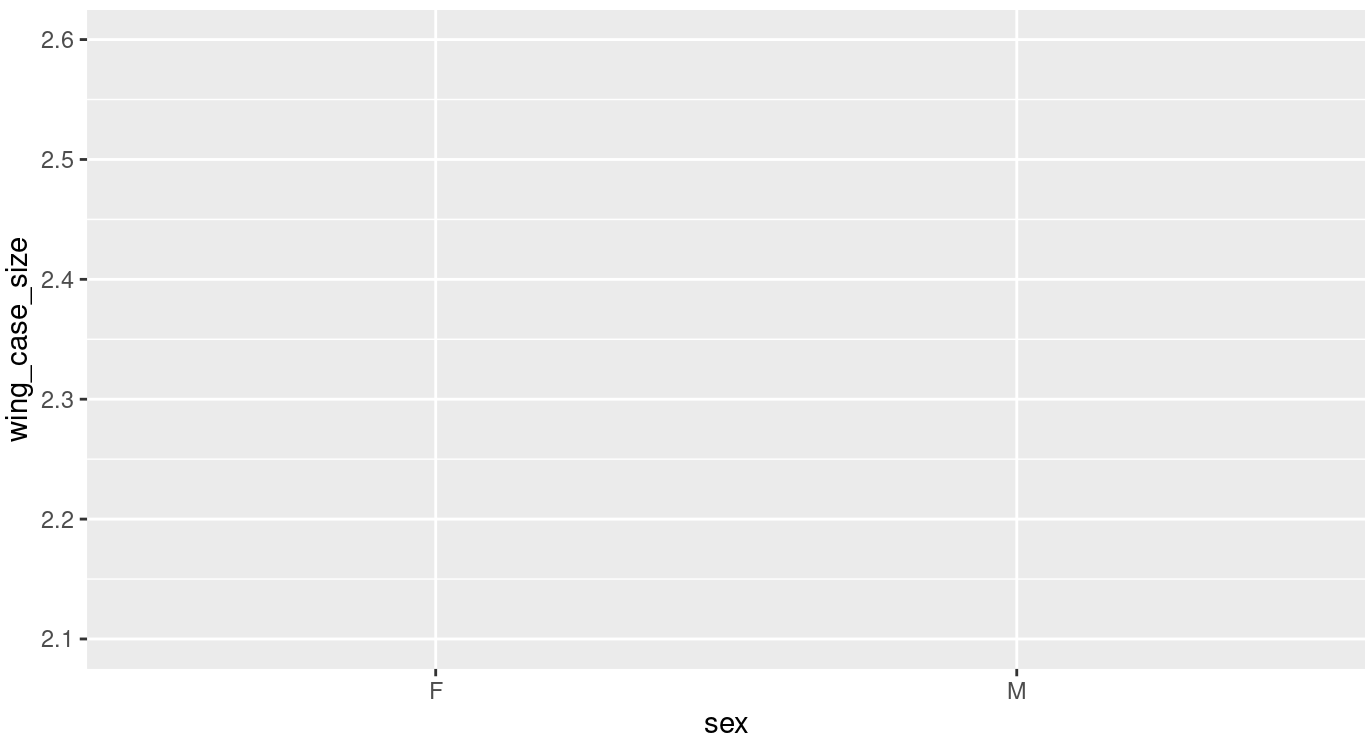
\includegraphics[width=0.9\linewidth]{figures/screenshot_deconstructingaplot_1} \caption{The most basic output from ggplot}\label{fig:unnamed-chunk-50}
\end{figure}

Now modify the script so that it looks like this\ldots{}

\begin{Shaded}
\begin{Highlighting}[]
\CommentTok{\# Making a box plot and saving it in an object}
\CommentTok{\# Call the ggplot function and direct it to your data and define your x axis and y axis}
\NormalTok{size\_differences\_boxplot }\OtherTok{\textless{}{-}} \FunctionTok{ggplot}\NormalTok{(}\AttributeTok{data =}\NormalTok{ tribolium\_combo,}\FunctionTok{aes}\NormalTok{(}\AttributeTok{x =}\NormalTok{ sex, }\AttributeTok{y =}\NormalTok{ wing\_case\_size)) }\SpecialCharTok{+} 
  \FunctionTok{geom\_boxplot}\NormalTok{(}\FunctionTok{aes}\NormalTok{(}\AttributeTok{fill =}\NormalTok{ treatment)) }\CommentTok{\# Tell ggplot that you want it to build a box plot coloured by treatment}
\FunctionTok{print}\NormalTok{(size\_differences\_boxplot) }\CommentTok{\# Print the object your plot is stored in to view it}
\end{Highlighting}
\end{Shaded}

Note the \texttt{+}, this is essentially another way of piping information from one function into the next. You could also have added \texttt{fill\ =\ treatment} to the first line within this chunk within \texttt{aes()}.

Your figure should look like this\ldots{}

\begin{figure}
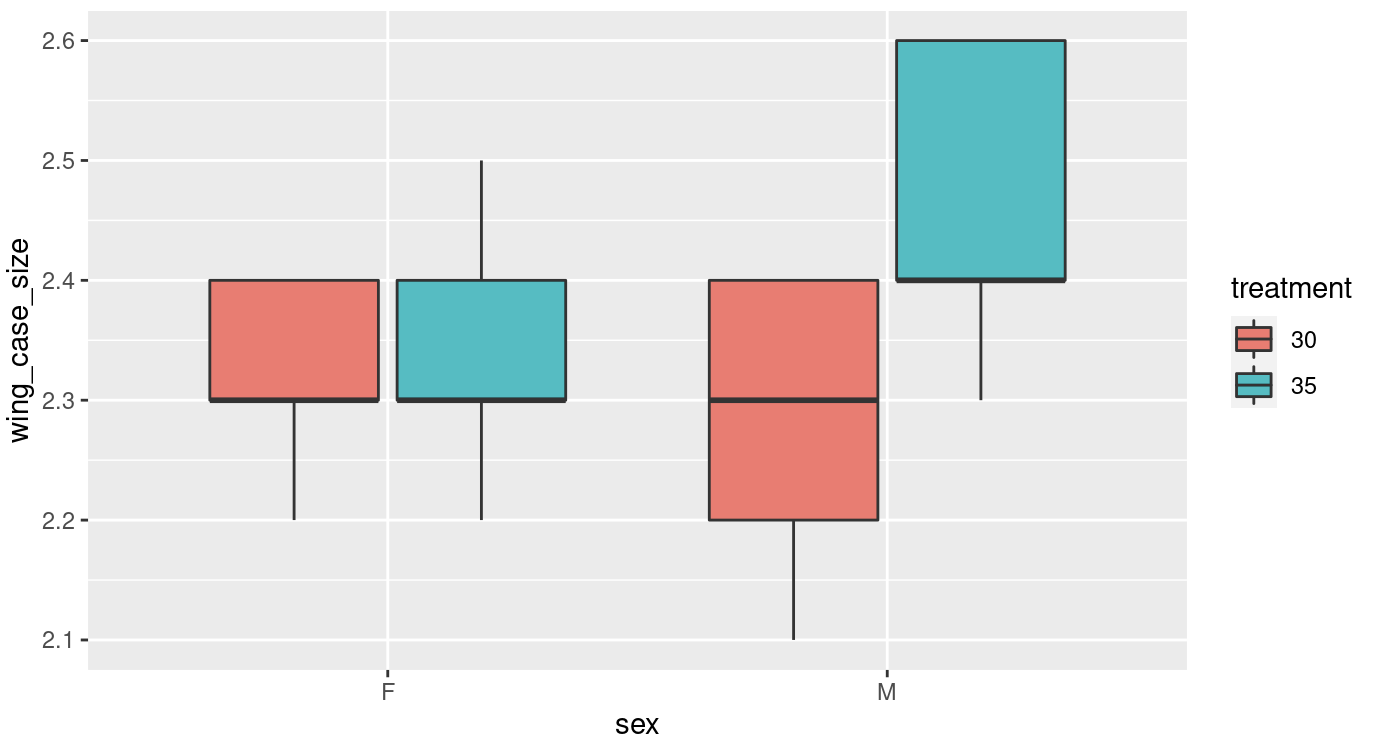
\includegraphics[width=0.9\linewidth]{figures/screenshot_deconstructingaplot_2} \caption{A basic ggplot box plot output}\label{fig:unnamed-chunk-52}
\end{figure}

Have a look at this figure, is there anything you would change, to make it more visually appealing or clear?

Here are some things I would change:

\begin{itemize}
\tightlist
\item
  Labels
\item
  Colour scheme
\item
  Spacing
\item
  Theme
\end{itemize}

We will look into labels and colour scheme this week and spacing and theme next week.

\hypertarget{labels}{%
\section{Labels}\label{labels}}

Clear accurate labeling is essential in the sciences, be it when your in the lab labeling up your samples or creating data visualisations.

In our current plot both our x and y axis could do with some relabeling, just because we dont use capitals when coding doesn't mean we don't follow the normal rules of English grammar when presenting data. Try adjusting your code so that it looks like the following;

\begin{Shaded}
\begin{Highlighting}[]
\CommentTok{\# Making a box plot and saving it in an object}
\CommentTok{\# Call the ggplot function and direct it to your data and define your x axis and y axis}
\NormalTok{size\_differences\_boxplot }\OtherTok{\textless{}{-}} \FunctionTok{ggplot}\NormalTok{(}\AttributeTok{data =}\NormalTok{ tribolium\_combo,}\FunctionTok{aes}\NormalTok{(}\AttributeTok{x =}\NormalTok{ sex, }\AttributeTok{y =}\NormalTok{ wing\_case\_size)) }\SpecialCharTok{+} 
  \FunctionTok{geom\_boxplot}\NormalTok{(}\FunctionTok{aes}\NormalTok{(}\AttributeTok{fill =}\NormalTok{ treatment)) }\SpecialCharTok{+} \CommentTok{\# Tell ggplot that you want it to build a boxplot}
  \FunctionTok{labs}\NormalTok{(}\AttributeTok{x =} \StringTok{"Sex"}\NormalTok{, }\AttributeTok{y =} \StringTok{"Wing case size (mm)}\SpecialCharTok{\textbackslash{}n}\StringTok{"}\NormalTok{) }\CommentTok{\# Adjust your x and y axis labels }
\FunctionTok{print}\NormalTok{(size\_differences\_boxplot) }\CommentTok{\# Print the object your plot is stored in to view it}
\end{Highlighting}
\end{Shaded}

Note the \texttt{\textbackslash{}n} on your y axis label. This simply adds a new line to the label and spaces it nicely away from the y axis.

This looks a bit better but our legend is still not very well labeled. Adjust your \texttt{labs} function so that it reads \texttt{labs(x\ =\ "Sex",\ y\ =\ "Wing\ case\ size\ (mm)\textbackslash{}n",\ fill\ =\ "Treatment")}. This will change the label for your legend.

Our labels still aren't quite right, I don't like the abbreviations on the x axis and our legend could still use some work as there are no units given for the treatment temperatures. Try these changes;

\begin{Shaded}
\begin{Highlighting}[]
\CommentTok{\# Making a box plot and saving it in an object}
\CommentTok{\# Call the ggplot function and direct it to your data and define your x axis and y axis}
\NormalTok{size\_differences\_boxplot }\OtherTok{\textless{}{-}} \FunctionTok{ggplot}\NormalTok{(}\AttributeTok{data =}\NormalTok{ tribolium\_combo,}\FunctionTok{aes}\NormalTok{(}\AttributeTok{x =}\NormalTok{ sex, }\AttributeTok{y =}\NormalTok{ wing\_case\_size)) }\SpecialCharTok{+} 
  \FunctionTok{geom\_boxplot}\NormalTok{(}\FunctionTok{aes}\NormalTok{(}\AttributeTok{fill =}\NormalTok{ treatment)) }\SpecialCharTok{+} \CommentTok{\# Tell ggplot that you want it to build a boxplot}
  \FunctionTok{labs}\NormalTok{(}\AttributeTok{x =} \StringTok{"Sex"}\NormalTok{, }\AttributeTok{y =} \StringTok{"Wing case size (mm)}\SpecialCharTok{\textbackslash{}n}\StringTok{"}\NormalTok{, }\AttributeTok{fill =} \StringTok{"Treatment"}\NormalTok{) }\SpecialCharTok{+} \CommentTok{\# Adjust your legend and x and y axis labels }
  \FunctionTok{scale\_x\_discrete}\NormalTok{(}\AttributeTok{labels =} \FunctionTok{c}\NormalTok{(}\StringTok{"Female"}\NormalTok{,}\StringTok{"Male"}\NormalTok{)) }\SpecialCharTok{+} \CommentTok{\# Rename the categories on the x axis }
  \FunctionTok{scale\_fill\_manual}\NormalTok{(}\AttributeTok{labels =} \FunctionTok{c}\NormalTok{(}\StringTok{"30°C"}\NormalTok{, }\StringTok{"35°C"}\NormalTok{)) }\CommentTok{\# Rename your treatments}
\FunctionTok{print}\NormalTok{(size\_differences\_boxplot) }\CommentTok{\# Print the object your plot is stored in to view it}
\end{Highlighting}
\end{Shaded}

Note that the \texttt{scale\ x\ discrete} and \texttt{scale\_fill\_manual} functions simply rename things in the same order as you present them, make sure you label your categories accurately or this can make a big mess later on.

If you try to remake your plot at this stage you will get the following error:

\begin{verbatim}
Error in `f()`:
! Insufficient values in manual scale. 2 needed but only 0 provided.
Run `rlang::last_error()` to see where the error occurred.
\end{verbatim}

This is because \texttt{scale\_fill\_manual} is also expecting some instructions on how to colour your boxplot. You will need to complete Chapter \ref{colours} before you can successfully remake your boxplot.

\hypertarget{colours}{%
\section{Switching up colours}\label{colours}}

The colours of your boxes are the default colours given by \texttt{ggplot2}. We can modify these to make our plot look a bit more pleasing. Try editing the \texttt{scale\_fill\_manual} function to this \texttt{scale\_fill\_manual(labels\ =\ c("30°C",\ "35°C"),\ values\ =\ c("cornflowerblue",\ "coral"))}. Run it and see what happens to your plot.

What do you think of your new plot now? Do you think the changes to labels and colours are an improvement?

R has lots of \href{https://www.datanovia.com/en/blog/awesome-list-of-657-r-color-names/}{colours}, take a look at the linked reference lists and have a play with changing up some of your colours.

Colour can be a really useful tool to employ when making your plots visually appealing, however make sure you are mindful that some colour pallets can be difficult for some people to interpret. There are however, some really good \href{https://www.tableau.com/en-gb/about/blog/examining-data-viz-rules-dont-use-red-green-together\#:~:text=Use\%20a\%20colour\%2Dblind\%2Dfriendly\%20palette\%20when\%20appropriate\&text=For\%20example\%2C\%20blue\%2Forange\%20is,blue\%20to\%20someone\%20with\%20CVD}{tips} out there for making sure your figures are accessible to everyone.

\hypertarget{before-you-leave-4}{%
\section{Before you leave!}\label{before-you-leave-4}}

Log out of posit Cloud and make sure you save your script!

\hypertarget{references-5}{%
\section{References}\label{references-5}}

Wickham, Hadley, Mara Averick, Jennifer Bryan, Winston Chang, Lucy D'Agostino McGowan, Romain François, Garrett Grolemund, et al.~2019. ``Welcome to the tidyverse.'' Journal of Open Source Software 4 (43): 1686. \url{https://doi.org/10.21105/joss.01686}.
Wickham, Hadley, Winston Chang, Lionel Henry, Thomas Lin Pedersen, Kohske Takahashi, Claus Wilke, Kara Woo, Hiroaki Yutani, and Dewey Dunnington. 2021. Ggplot2: Create Elegant Data Visualisations Using the Grammar of Graphics. \url{https://CRAN.R-project.org/package=ggplot2}.

\hypertarget{pretty-figs-p2}{%
\chapter{Make them pretty continued - Week 10A}\label{pretty-figs-p2}}

You should aim to complete this chapter in Week 10, Semester 1

In Chapter \ref{pretty-figs-p1} we explored the fundamental functionality of \texttt{ggplot2} and we started to play with some functions that improved our plots labels and colour scheme. This week we will be extending this further and investigating how we may also be able to alter spacing and themes to improve the appearance of our plots.

Open your \texttt{tribolium\_parasites} project in posit Cloud and your \texttt{ggplot\_fundamentals.r} script.

Your current figure chunk should look something like this;

\begin{Shaded}
\begin{Highlighting}[]
\CommentTok{\# Making a box plot and saving it in an object}
\CommentTok{\# Call the ggplot function and direct it to your data and define your x axis and y axis}
\NormalTok{size\_differences\_boxplot }\OtherTok{\textless{}{-}} \FunctionTok{ggplot}\NormalTok{(}\AttributeTok{data =}\NormalTok{ tribolium\_combo,}\FunctionTok{aes}\NormalTok{(}\AttributeTok{x =}\NormalTok{ sex, }\AttributeTok{y =}\NormalTok{ wing\_case\_size)) }\SpecialCharTok{+} 
  \FunctionTok{geom\_boxplot}\NormalTok{(}\FunctionTok{aes}\NormalTok{(}\AttributeTok{fill =}\NormalTok{ treatment)) }\SpecialCharTok{+} \CommentTok{\# Tell ggplot that you want it to build a box plot filled according to treatment}
  \FunctionTok{labs}\NormalTok{(}\AttributeTok{x =} \StringTok{"Sex"}\NormalTok{, }\AttributeTok{y =} \StringTok{"Wing case size (mm)}\SpecialCharTok{\textbackslash{}n}\StringTok{"}\NormalTok{, }\AttributeTok{fill =} \StringTok{"Treatment"}\NormalTok{) }\SpecialCharTok{+} \CommentTok{\# Adjust your legend and x and y axis labels }
  \FunctionTok{scale\_x\_discrete}\NormalTok{(}\AttributeTok{labels =} \FunctionTok{c}\NormalTok{(}\StringTok{"Female"}\NormalTok{,}\StringTok{"Male"}\NormalTok{)) }\SpecialCharTok{+} \CommentTok{\# Rename the categories on the x axis }
  \FunctionTok{scale\_fill\_manual}\NormalTok{(}\AttributeTok{labels =} \FunctionTok{c}\NormalTok{(}\StringTok{"30°C"}\NormalTok{, }\StringTok{"35°C"}\NormalTok{), }\AttributeTok{values =} \FunctionTok{c}\NormalTok{(}\StringTok{"cornflowerblue"}\NormalTok{, }\StringTok{"coral"}\NormalTok{)) }\CommentTok{\# Rename and colour your treatments}
\FunctionTok{print}\NormalTok{(size\_differences\_boxplot) }\CommentTok{\# Print the object your plot is stored in to view it}
\end{Highlighting}
\end{Shaded}

\hypertarget{spacing}{%
\section{Spacing}\label{spacing}}

Lets have a look at spacing. This is a box plot so we the main spacing option you are likely to want to play with is the width of your boxes. Here we can simply add an argument to the \texttt{geom\_boxplot} function. Edit this function so that it reads \texttt{geom\_boxplot(aes(fill\ =\ treatment),\ width\ =\ 0.9)}. The width argument can be anything between 0.00 or 1.00. It changes the width of the boxes and this changes the spacing between them as well. Have a play with some values and see what happens.

We will come back to spacing when we look at our scatter plots next week.

\hypertarget{themes}{%
\section{Themes}\label{themes}}

So the final aspect of aesthetics we are going to look at here is themes. We have a reasonably attractive graph now, but its still got a grey background and the grid lines are unnecessary. To remove the grey background and implement the classic black on white aesthetic we can simply add a function that defines a pre-made theme. Adjust your script so that it includes the function \texttt{theme\_bw()}, I suggest you add this as a new line, don't forget to pipe between your functions with a \texttt{+}. Run this chunk and print your new plot. How is that looking now?

Two things still jump out at me when looking at this plot. The grid lines are completely unnecessary and detract from the overall aesthetic and the text sizes could be larger. To make these edits we can simply add additional instructions to adjust the theme further. So although most of the work has been done by applying a the \texttt{theme\_bw} we still need make some adjustments.

Add the following function to your growing ggplot chunk (don't forget to pipe \texttt{+} between functions);

\begin{Shaded}
\begin{Highlighting}[]
\FunctionTok{theme}\NormalTok{(}\AttributeTok{panel.border =} \FunctionTok{element\_rect}\NormalTok{(}\AttributeTok{color=}\StringTok{"black"}\NormalTok{), }\CommentTok{\# Specifies that the plot boarder is coloured black}
        \AttributeTok{panel.grid.minor =} \FunctionTok{element\_blank}\NormalTok{(), }\CommentTok{\# Removes minor grid lines }
        \AttributeTok{panel.grid.major =} \FunctionTok{element\_blank}\NormalTok{()) }\CommentTok{\# Removes major grid lines }
\end{Highlighting}
\end{Shaded}

Now we just need to adjust the text size. We can do this within the \texttt{theme} function as well adjust your theme so that it reads like this;

\begin{Shaded}
\begin{Highlighting}[]
\FunctionTok{theme}\NormalTok{(}\AttributeTok{panel.border =} \FunctionTok{element\_rect}\NormalTok{(}\AttributeTok{color=}\StringTok{"black"}\NormalTok{), }\CommentTok{\# Specifies that the plot boarder is coloured black}
        \AttributeTok{panel.grid.minor =} \FunctionTok{element\_blank}\NormalTok{(), }\CommentTok{\# Removes minor grid lines }
        \AttributeTok{panel.grid.major =} \FunctionTok{element\_blank}\NormalTok{(), }\CommentTok{\# Removes major grid lines }
        \AttributeTok{axis.text =} \FunctionTok{element\_text}\NormalTok{(}\AttributeTok{size =} \DecValTok{15}\NormalTok{), }\CommentTok{\# Changes the size of text on both axis }
        \AttributeTok{axis.title =} \FunctionTok{element\_text}\NormalTok{(}\AttributeTok{size =} \DecValTok{20}\NormalTok{), }\CommentTok{\# Changes size of your axis labels }
        \AttributeTok{legend.text =} \FunctionTok{element\_text}\NormalTok{(}\AttributeTok{size =} \DecValTok{15}\NormalTok{), }\CommentTok{\# Changes the size of text within your legend}
        \AttributeTok{legend.title =} \FunctionTok{element\_text}\NormalTok{(}\AttributeTok{size =} \DecValTok{20}\NormalTok{)) }\CommentTok{\# Changes the size of the legend title}
\end{Highlighting}
\end{Shaded}

Have a play with the different text sizes until you think they are optimal.

Hopefully you now have a nice clean, clear and aesthetically pleasing plot and have some awareness of the commands and functions used to make it. Next week is our last workshop of the term and we will be applying these rules to all of the plots made in the previous chapters. This will also give you the oppotunity to ask any questions.

\hypertarget{before-you-leave-5}{%
\section{Before you leave!}\label{before-you-leave-5}}

Log out of posit Cloud and make sure you save your script!

\hypertarget{references-6}{%
\section{References}\label{references-6}}

Wickham, Hadley, Mara Averick, Jennifer Bryan, Winston Chang, Lucy D'Agostino McGowan, Romain François, Garrett Grolemund, et al.~2019. ``Welcome to the tidyverse.'' Journal of Open Source Software 4 (43): 1686. \url{https://doi.org/10.21105/joss.01686}.
Wickham, Hadley, Winston Chang, Lionel Henry, Thomas Lin Pedersen, Kohske Takahashi, Claus Wilke, Kara Woo, Hiroaki Yutani, and Dewey Dunnington. 2021. Ggplot2: Create Elegant Data Visualisations Using the Grammar of Graphics. \url{https://CRAN.R-project.org/package=ggplot2}.

\hypertarget{cannibalisation}{%
\chapter{The subtle art of cannibalisation - Week 11A - Workshop 3}\label{cannibalisation}}

In this Week 11 workshop we will be applying the rules of aesthetics that we learned in the last two chapters to the rest of our plots. You may use functions and arguments from your \texttt{ggplot\_fundamentals.r} script to modify the plots you made in previous weeks. This is a very common practice, especially while learning a new programming language, you get a script or chunk of code right once and then canibalise parts of it for other uses, modifying it as needed to fit its new purpose.

\hypertarget{starting-on-the-right-footing}{%
\section{Starting on the right footing}\label{starting-on-the-right-footing}}

In the last few chapters, and over the last few weeks you have been asked to modify quite a few chunks of script. If anything hasn't made sense or you haven't managed to get some chunks or functions working please do let either myself or a demonstrator know before you start the workshop activity. We are here to help!

\hypertarget{beautifying-your-box-plots}{%
\section{Beautifying your box plots}\label{beautifying-your-box-plots}}

In Chapters 9 and 10 we specifically worked on making changes to our box plots that would make them clean, clear and visually pleasing. You have all the code already made for your box plots, it just needs tailoring a little. You should have three boxplots saved in your \texttt{figures} folder (made in Chapter \ref{boxplot});

\begin{itemize}
\tightlist
\item
  size\_differences\_by\_sex\_boxplot.pdf
\item
  size\_differences\_by\_treatment\_boxplot.pdf
\item
  size\_differences\_boxplot.pdf - remember this is filled by \texttt{sex} not \texttt{treatment} so will be subtly different to the figure made in the \texttt{ggplot\_fundamentals.R}.
\end{itemize}

Using the script from \texttt{ggplot\_fundamentals.R} make the necessary modifications to each of these three figures so that they are clean, clear and visually pleasing. Make sure you save each one to your \texttt{figures} folder using \texttt{ggsave}.

\hypertarget{beautifying-your-histograms}{%
\section{Beautifying your histograms}\label{beautifying-your-histograms}}

You hopefully also have two histograms saved in your \texttt{figures} folder (made in Chapter \ref{histogram});

\begin{itemize}
\tightlist
\item
  size\_histogram.pdf
\item
  parasite\_histogram.pdf
\end{itemize}

Use you previous chunks of scripts and knowledge of R to edit the labels and themes of this plot. Print it again and take a look. When you're happy save your updated figures to the \texttt{figures} folder using \texttt{ggsave}.

\hypertarget{beautifying-your-scatter-plot}{%
\section{Beautifying your scatter plot}\label{beautifying-your-scatter-plot}}

You hopefully also have a scatter plot saved in your \texttt{figures} folder (made in Chapter \ref{scatter});

\begin{itemize}
\tightlist
\item
  size\_vs\_parasites\_point.pdf
\end{itemize}

Use you previous chunks of scripts and knowledge of R to edit the labels and themes of this plot. Print it again and take a look.

Now there are some additional elements in this plot that could be adjusted. These include;

\begin{itemize}
\tightlist
\item
  Point shape - The shape of the individual points on the plot, as with colours there are lots of options numbered 0 - 25, descriptions of each one are listed \href{https://www.datanovia.com/en/blog/ggplot-point-shapes-best-tips/}{here}
\item
  Point size - The size of each point
\item
  Point colour - The colour of your points
\item
  Line type (solid, dashed, etc) - Again thre are several options here, the notation and descriptions of which can be found \href{http://www.sthda.com/english/wiki/ggplot2-line-types-how-to-change-line-types-of-a-graph-in-r-software}{here}
\item
  Line colour
\item
  Line size - the weight of the line
\item
  Line fill - Note that here this refers to the colour of the shaded area marking the standard error
\end{itemize}

So lets play with some of these. Try adding and adjusting the following arguments within \texttt{geom\_point()}

\begin{itemize}
\tightlist
\item
  \texttt{shape\ =\ 1} - have a look at other point shapes you could use and play with this setting
\item
  \texttt{size\ =\ 2} - again try playing with some point sizes
\item
  \texttt{colour\ =\ "blue"} - or any other \href{https://www.datanovia.com/en/blog/awesome-list-of-657-r-color-names/}{colour} you fancy trying.
\end{itemize}

Once you are happy with your points we can take a look at your regression line. Try adding and adjusting the following arguments within \texttt{geom\_smooth()}

\begin{itemize}
\tightlist
\item
  \texttt{colour\ =\ "cornflowerblue"}
\item
  \texttt{fill\ =\ "lightblue"}
\item
  \texttt{size\ =\ 1}
\item
  \texttt{linetype\ =\ "dashed"}
\end{itemize}

As before please do experiment and play with the settings described by each of these arguments.

Once you are happy with your new and beautiful scatter plot make sure you save it to to the \texttt{figures} folder using \texttt{ggsave}.

\hypertarget{a-challenge}{%
\section{A Challenge!}\label{a-challenge}}

Try to adjust the chunk for your size vs parasites scatter plot so that the points are coloured by \texttt{sex} and shaped by \texttt{treatment}. Colour female points \texttt{"deepskyblue3"} and male points \texttt{"coral"} and use solid squares for the 30°C treatment and solid circles for the 35°C treatment. Make sure the text and titles for your legends are correct and well presented.

Hint - to do this you will need to correctly use and populate the \texttt{aes()} function in \texttt{geom\_point()} and then to adjust colours, shapes and associated text you will need to pipe \texttt{+} to the \texttt{scale\_color\_manual()} and the \texttt{scale\_shape\_manual()} functions. You will also need to adjust the settings in the \texttt{labs()} function to change the legend titles.

\hypertarget{formative-assignment}{%
\section{Formative Assignment}\label{formative-assignment}}

This is the last of the taught content for the Introduction to Data Science sub module. You should all be very proud of yourselves for completing the first half of this workbook! You now have the opportunity to submit a formative assignment, this is hosted in PebblePad and can be accessed through the BIO-4008Y page on blackboard in the Data Science Learning Module. Details of the task can be found in Chapter \ref{formative}.

See you all in the new year :)

\hypertarget{before-you-leave-6}{%
\section{Before you leave!}\label{before-you-leave-6}}

Log out of posit Cloud and make sure you save your script!

\hypertarget{references-7}{%
\section{References}\label{references-7}}

Wickham, Hadley, Mara Averick, Jennifer Bryan, Winston Chang, Lucy D'Agostino McGowan, Romain François, Garrett Grolemund, et al.~2019. ``Welcome to the tidyverse.'' Journal of Open Source Software 4 (43): 1686. \url{https://doi.org/10.21105/joss.01686}.
Wickham, Hadley, Winston Chang, Lionel Henry, Thomas Lin Pedersen, Kohske Takahashi, Claus Wilke, Kara Woo, Hiroaki Yutani, and Dewey Dunnington. 2021. Ggplot2: Create Elegant Data Visualisations Using the Grammar of Graphics. \url{https://CRAN.R-project.org/package=ggplot2}.

\hypertarget{formative}{%
\chapter{Formative Assessment - Deadline 15/12/23}\label{formative}}

The formative assessment is essentially a stripped down version of what will be asked for in the summative assessment task. Both formative and summative task will be marked similarly, so this is a fantastic opportunity to get feedback on this section of the Skills modules. There are essentially two tasks for the formative.

\hypertarget{task-1}{%
\section{Task 1 - Figure and Figure Legend}\label{task-1}}

Download one of your \texttt{.pdf} box plots or scatter plots from posit Cloud, it doesnt matter which one but it does need to be presented well. Plot selection and presentation will be assessed. Use the tips and tricks that we covered in Chapters \ref{pretty-figs-p1}, \ref{pretty-figs-p2} and \ref{cannibalisation}. You can download your files from posit Cloud onto your local device by moving to your \texttt{figures} folder, ticking the box next to the file you wish to download and then clicking on \texttt{More} and then \texttt{Export}. You will then be given the option to \texttt{Download} your files. Once you have your figure of choice downloaded you can copy it into a Word file and write a suitable figure legend.

Remember my top tips for writing an appropriate figure legend (as covered in lectures);

Legends \textbf{should};

\begin{itemize}
\tightlist
\item
  Allow the reader to understand the figure without reference to the text, so include information about what is being shown. For example, with a box plot you may wish to say ``The middle line, box and whiskers represent the median, interquartile range and range, respectively.''
\item
  Include info on sample size, study organism (in Latin) and (if relevant, e.g.~ecology) study location and time
\end{itemize}

Legends \textbf{should NOT};

\begin{itemize}
\tightlist
\item
  Include information that is obvious to a scientific audience (e.g.~``a scatter plot to show'' or ``a graph to show'')
\item
  Repeat what's in the figure (e.g.~describe what the colour mean if you also have a key in the figure)
\end{itemize}

\hypertarget{task-2---script}{%
\section{Task 2 - Script}\label{task-2---script}}

Hopefully you have been keeping your script nice and clean and tidy throughout your \texttt{tribolium\_parasites} analysis and have it saved nicely in your \texttt{scripts} folder. If you have then this step will be super easy! You simply need to download your script using the same method described above in Chapter \ref{task-1}.

\hypertarget{task-3---submission}{%
\section{Task 3 - Submission}\label{task-3---submission}}

If you go to the Data Sciences Learning Module in the BIO-4008Y page of blackboard you will see a link to PebblePad. If you follow this link you should be automatically taken to the Data Sciences portfolio. You will see there are two pages to the portfolio, at this stage you only need to complete the \texttt{Formative} page. You will see there are a number of tick boxes to help guide you through what our expectations are from your work here. There are then two places to upload your work, one for your figure and figure legend and the other for your script. Upload the corresponding documents where required.

You may notice that there is a check box where you will need to assert that this is your own work. Once this is done you can scroll down and you will be able to mark the page as complete. Once you have marked your page as complete you can consider it submitted.

\begin{quote}
Top tip - as you scroll down the page you can see that there is a marking rubric included, these are the criteria under which we will be marking your work, a similar one has been created for the summative page as well.
\end{quote}

The deadline for formative submissions is the 8/12/23, I will mark all submissions submitted by this date over the Christmas break.

\hypertarget{code}{%
\chapter{Merry Christmas!!!}\label{code}}

You have all done fanatically well in semester A so I have got you all a lovely Christmas gift\ldots{} Fully commented and completed versions of the scripts you have been working on. I would still suggest you try to complete the workbook in your own time, this will mean that you have a much better understanding of how the code works and will be better for you in the long run. But these commented and completed scripts may give you something to compare your own work too and will hopefully allow us all to start on the same page in the New Year.

\textbf{Show me the Tribolium parasites script}

\begin{Shaded}
\begin{Highlighting}[]
\CommentTok{\# An analysis of parasite abundance between male and female tribolium beetles from two thermal treatments (30 and 35 degrees centigrade)}
\CommentTok{\# Ellen Bell }
\CommentTok{\# 08/08/2022}

\FunctionTok{library}\NormalTok{(tidyverse) }\CommentTok{\# Loads the tidyverse package}
\FunctionTok{library}\NormalTok{(janitor) }\CommentTok{\# Loads the janitor package}

\CommentTok{\# Read the data from the .csv file in the data folder into my project}
\NormalTok{tribolium }\OtherTok{\textless{}{-}} \FunctionTok{read\_csv}\NormalTok{(}\StringTok{"data/Tribolium\_parasites.csv"}\NormalTok{) }\CommentTok{\#}

\FunctionTok{head}\NormalTok{(tribolium)}

\CommentTok{\# First of all lets create some variables}
\NormalTok{beetle\_id }\OtherTok{\textless{}{-}} \FunctionTok{c}\NormalTok{(}\DecValTok{1}\SpecialCharTok{:}\DecValTok{20}\NormalTok{) }\CommentTok{\# Notice that this notation will create of a list of numbers 1 to 20}
\NormalTok{sex }\OtherTok{\textless{}{-}} \FunctionTok{c}\NormalTok{(}\StringTok{"F"}\NormalTok{,}\StringTok{"F"}\NormalTok{,}\StringTok{"F"}\NormalTok{,}\StringTok{"F"}\NormalTok{,}\StringTok{"F"}\NormalTok{,}\StringTok{"M"}\NormalTok{,}\StringTok{"M"}\NormalTok{,}\StringTok{"M"}\NormalTok{,}\StringTok{"M"}\NormalTok{,}\StringTok{"M"}\NormalTok{,}\StringTok{"F"}\NormalTok{,}\StringTok{"F"}\NormalTok{,}\StringTok{"F"}\NormalTok{,}\StringTok{"F"}\NormalTok{,}\StringTok{"F"}\NormalTok{,}\StringTok{"M"}\NormalTok{,}\StringTok{"M"}\NormalTok{,}\StringTok{"M"}\NormalTok{,}\StringTok{"M"}\NormalTok{,}\StringTok{"M"}\NormalTok{)}
\NormalTok{treatment }\OtherTok{\textless{}{-}} \FunctionTok{c}\NormalTok{(}\DecValTok{35}\NormalTok{,}\DecValTok{35}\NormalTok{,}\DecValTok{35}\NormalTok{,}\DecValTok{35}\NormalTok{,}\DecValTok{35}\NormalTok{,}\DecValTok{35}\NormalTok{,}\DecValTok{35}\NormalTok{,}\DecValTok{35}\NormalTok{,}\DecValTok{35}\NormalTok{,}\DecValTok{35}\NormalTok{,}\DecValTok{30}\NormalTok{,}\DecValTok{30}\NormalTok{,}\DecValTok{30}\NormalTok{,}\DecValTok{30}\NormalTok{,}\DecValTok{30}\NormalTok{,}\DecValTok{30}\NormalTok{,}\DecValTok{30}\NormalTok{,}\DecValTok{30}\NormalTok{,}\DecValTok{30}\NormalTok{,}\DecValTok{30}\NormalTok{)}

\CommentTok{\# Turning variables into a tibble}
\NormalTok{tribolium\_extras }\OtherTok{\textless{}{-}} \FunctionTok{tibble}\NormalTok{(beetle\_id,sex,treatment)}

\CommentTok{\# Renaming some variables in your original data set}
\NormalTok{tribolium }\OtherTok{\textless{}{-}}\NormalTok{ tribolium }\SpecialCharTok{\%\textgreater{}\%}
  \FunctionTok{rename}\NormalTok{(}\AttributeTok{beetle\_id =}\NormalTok{ beetle\_id)}
\NormalTok{tribolium }\OtherTok{\textless{}{-}}\NormalTok{ tribolium }\SpecialCharTok{\%\textgreater{}\%}
  \FunctionTok{rename}\NormalTok{(}\AttributeTok{wing\_case\_size =}\NormalTok{ wing\_case\_size)}
\NormalTok{tribolium }\OtherTok{\textless{}{-}}\NormalTok{ tribolium }\SpecialCharTok{\%\textgreater{}\%}
  \FunctionTok{rename}\NormalTok{(}\AttributeTok{parasite\_burden =}\NormalTok{ parasite\_burden)}

\CommentTok{\# Check how your data frame now looks}
\FunctionTok{head}\NormalTok{(tribolium)}

\CommentTok{\# Merge data frames}
\NormalTok{tribolium\_combo }\OtherTok{\textless{}{-}} \FunctionTok{merge}\NormalTok{(tribolium, tribolium\_extras, }\AttributeTok{by =} \StringTok{"beetle\_id"}\NormalTok{) }\CommentTok{\# This merge function combines both of your data frames but matches rows by beetle\_id}

\FunctionTok{glimpse}\NormalTok{(tribolium\_combo)}

\CommentTok{\# Save your combined data frame as a .csv file (which you could download) to your data folder}
\FunctionTok{write.csv}\NormalTok{(tribolium\_combo,}\StringTok{"data/tribolium\_combo.csv"}\NormalTok{, }\AttributeTok{row.names =} \ConstantTok{FALSE}\NormalTok{)}

\CommentTok{\# Use the n\_distinct function to count unique/distinct entries in the beetle\_id column}
\FunctionTok{n\_distinct}\NormalTok{(tribolium\_combo}\SpecialCharTok{$}\NormalTok{beetle\_id)}

\CommentTok{\# Use the tabyl function from the janitor package, comment on what it does. }
\FunctionTok{tabyl}\NormalTok{(tribolium\_combo, sex , treatment)}

\CommentTok{\# Making a histogram and saving it in an object}
\CommentTok{\# Call the ggplot function and direct it to your data and define your x axis}
\NormalTok{size\_histogram }\OtherTok{\textless{}{-}} \FunctionTok{ggplot}\NormalTok{(}\AttributeTok{data =}\NormalTok{ tribolium\_combo,}\FunctionTok{aes}\NormalTok{(}\AttributeTok{x =}\NormalTok{ wing\_case\_size)) }\SpecialCharTok{+} 
  \FunctionTok{geom\_histogram}\NormalTok{(}\AttributeTok{bins =} \DecValTok{6}\NormalTok{) }\CommentTok{\# Tell ggplot that you want it to build a histogram with 6 equal sized bins}
\FunctionTok{print}\NormalTok{(size\_histogram) }\CommentTok{\# Print your new figure}

\NormalTok{parasite\_burden\_histogram }\OtherTok{\textless{}{-}} \FunctionTok{ggplot}\NormalTok{(}\AttributeTok{data =}\NormalTok{ tribolium\_combo,}\FunctionTok{aes}\NormalTok{(}\AttributeTok{x =}\NormalTok{ parasite\_burden)) }\SpecialCharTok{+} 
  \FunctionTok{geom\_histogram}\NormalTok{(}\AttributeTok{bins =} \DecValTok{6}\NormalTok{) }\CommentTok{\# Tell ggplot that you want it to build a histogram with 6 equal sized bins}
\FunctionTok{print}\NormalTok{(parasite\_burden\_histogram) }\CommentTok{\# Print your new figure}

\CommentTok{\# Saving outputs}
\FunctionTok{ggsave}\NormalTok{(}\StringTok{"figures/tribolium\_wingcase\_size\_histogram.pdf"}\NormalTok{, }\CommentTok{\# Give R a path to save to and a file name}
       \AttributeTok{plot =}\NormalTok{ size\_histogram, }\CommentTok{\# Tell R what to save {-} in this case your object}
       \AttributeTok{device =} \StringTok{"pdf"}\NormalTok{) }\CommentTok{\# Tell R what file type to create, in this case a pdf}
\FunctionTok{ggsave}\NormalTok{(}\StringTok{"figures/tribolium\_parasite\_burden\_histogram.pdf"}\NormalTok{, }\CommentTok{\# Give R a path to save to and a file name}
       \AttributeTok{plot =}\NormalTok{ parasite\_burden\_histogram, }\CommentTok{\# Tell R what to save {-} in this case your object}
       \AttributeTok{device =} \StringTok{"pdf"}\NormalTok{) }\CommentTok{\# Tell R what file type to create, in this case a pdf}

\CommentTok{\# Making a box plot and saving it in an object}
\CommentTok{\# Call the ggplot function and direct it to your data and define your x axis and y axis}
\NormalTok{size\_differences\_by\_sex\_boxplot }\OtherTok{\textless{}{-}} \FunctionTok{ggplot}\NormalTok{(}\AttributeTok{data =}\NormalTok{ tribolium\_combo,}\FunctionTok{aes}\NormalTok{(}\AttributeTok{x =}\NormalTok{ sex, }\AttributeTok{y =}\NormalTok{ wing\_case\_size)) }\SpecialCharTok{+} 
  \FunctionTok{geom\_boxplot}\NormalTok{() }\CommentTok{\# Tell ggplot that you want it to build a boxplot}
\FunctionTok{print}\NormalTok{(size\_differences\_by\_sex\_boxplot) }\CommentTok{\# Print your new figure}

\CommentTok{\# Saving outputs}
\FunctionTok{ggsave}\NormalTok{(}\StringTok{"figures/size\_differences\_by\_sex\_boxplot.pdf"}\NormalTok{, }\CommentTok{\# Give R a path to save to and a file name}
       \AttributeTok{plot =}\NormalTok{ size\_differences\_by\_sex\_boxplot, }\CommentTok{\# Tell R what to save {-} in this case your object}
       \AttributeTok{device =} \StringTok{"pdf"}\NormalTok{) }\CommentTok{\# Tell R what file type to create, in this case a pdf}

\CommentTok{\# Instruct R to treat the treatment variable as a factor }
\NormalTok{tribolium\_combo}\SpecialCharTok{$}\NormalTok{treatment }\OtherTok{\textless{}{-}} \FunctionTok{as.factor}\NormalTok{(tribolium\_combo}\SpecialCharTok{$}\NormalTok{treatment) }\CommentTok{\# Note this will edit your data frame}

\CommentTok{\# Making a box plot and saving it in an object}
\CommentTok{\# Call the ggplot function and direct it to your data and define your x axis and y axis}
\NormalTok{size\_differences\_by\_treatment\_boxplot }\OtherTok{\textless{}{-}} \FunctionTok{ggplot}\NormalTok{(}\AttributeTok{data =}\NormalTok{ tribolium\_combo,}\FunctionTok{aes}\NormalTok{(}\AttributeTok{x =}\NormalTok{ treatment, }\AttributeTok{y =}\NormalTok{ wing\_case\_size)) }\SpecialCharTok{+} 
  \FunctionTok{geom\_boxplot}\NormalTok{() }\CommentTok{\# Tell ggplot that you want it to build a boxplot}
\FunctionTok{print}\NormalTok{(size\_differences\_by\_treatment\_boxplot) }\CommentTok{\# Print your new figure}

\CommentTok{\# Saving outputs}
\FunctionTok{ggsave}\NormalTok{(}\StringTok{"figures/size\_differences\_by\_treatment\_boxplot.pdf"}\NormalTok{, }\CommentTok{\# Give R a path to save to and a file name}
       \AttributeTok{plot =}\NormalTok{ size\_differences\_by\_treatment\_boxplot, }\CommentTok{\# Tell R what to save {-} in this case your object}
       \AttributeTok{device =} \StringTok{"pdf"}\NormalTok{) }\CommentTok{\# Tell R what file type to create, in this case a pdf}

\CommentTok{\# Making a box plot and saving it in an object}
\CommentTok{\# Call the ggplot function and direct it to your data and define your x axis and y axis}
\NormalTok{size\_differences\_by\_treatment\_and\_sex\_boxplot }\OtherTok{\textless{}{-}} \FunctionTok{ggplot}\NormalTok{(}\AttributeTok{data =}\NormalTok{ tribolium\_combo,}\FunctionTok{aes}\NormalTok{(}\AttributeTok{x =}\NormalTok{ treatment, }\AttributeTok{y =}\NormalTok{ wing\_case\_size, }\AttributeTok{fill =}\NormalTok{ sex)) }\SpecialCharTok{+} 
  \FunctionTok{geom\_boxplot}\NormalTok{() }\CommentTok{\# Tell ggplot that you want it to build a boxplot}
\FunctionTok{print}\NormalTok{(size\_differences\_by\_treatment\_and\_sex\_boxplot) }\CommentTok{\# Print your new figure}

\CommentTok{\# Saving outputs}
\FunctionTok{ggsave}\NormalTok{(}\StringTok{"figures/size\_differences\_by\_treatment\_and\_sex\_boxplot.pdf"}\NormalTok{, }\CommentTok{\# Give R a path to save to and a file name}
       \AttributeTok{plot =}\NormalTok{ size\_differences\_by\_treatment\_and\_sex\_boxplot, }\CommentTok{\# Tell R what to save {-} in this case your object}
       \AttributeTok{device =} \StringTok{"pdf"}\NormalTok{) }\CommentTok{\# Tell R what file type to create, in this case a pdf}

\CommentTok{\# Making a scatter plot and saving it in an object}
\CommentTok{\# Call the ggplot function and direct it to your data and define your x axis and y axis}
\NormalTok{size\_vs\_parasites\_point }\OtherTok{\textless{}{-}} \FunctionTok{ggplot}\NormalTok{(}\AttributeTok{data =}\NormalTok{ tribolium\_combo,}\FunctionTok{aes}\NormalTok{(}\AttributeTok{x =}\NormalTok{ wing\_case\_size , }\AttributeTok{y =}\NormalTok{ parasite\_burden )) }\SpecialCharTok{+} 
  \FunctionTok{geom\_point}\NormalTok{() }\SpecialCharTok{+} \CommentTok{\# geom\_point is ggplots scatter plot}
  \FunctionTok{geom\_smooth}\NormalTok{(}\AttributeTok{method=}\StringTok{"lm"}\NormalTok{)}
\FunctionTok{print}\NormalTok{(size\_vs\_parasites\_point)}

\CommentTok{\# Saving outputs}
\FunctionTok{ggsave}\NormalTok{(}\StringTok{"figures/size\_vs\_parsite\_point.pdf"}\NormalTok{, }\CommentTok{\# Give R a path to save to and a file name}
       \AttributeTok{plot =}\NormalTok{ size\_vs\_parasites\_point, }\CommentTok{\# Tell R what to save {-} in this case your object}
       \AttributeTok{device =} \StringTok{"pdf"}\NormalTok{) }\CommentTok{\# Tell R what file type to create, in this case a pdf}
\end{Highlighting}
\end{Shaded}

\textbf{Show me the ggplot fundamentals script}

\begin{Shaded}
\begin{Highlighting}[]
\CommentTok{\# ggplot fundamentals  }
\CommentTok{\# Ellen Bell }
\CommentTok{\# 08/08/2022}

\CommentTok{\# Clean up your environment}
\FunctionTok{rm}\NormalTok{(}\AttributeTok{list =} \FunctionTok{ls}\NormalTok{())}

\CommentTok{\# Reload your tribolium\_combo data frame}
\NormalTok{tribolium\_combo }\OtherTok{\textless{}{-}} \FunctionTok{read\_csv}\NormalTok{(}\StringTok{"data/tribolium\_combo.csv"}\NormalTok{)}

\CommentTok{\# Instruct R to treat the treatment variable as a factor }
\NormalTok{tribolium\_combo}\SpecialCharTok{$}\NormalTok{treatment }\OtherTok{\textless{}{-}} \FunctionTok{as.factor}\NormalTok{(tribolium\_combo}\SpecialCharTok{$}\NormalTok{treatment) }\CommentTok{\# Note this will edit your data frame}

\CommentTok{\# Making a box plot and saving it in an object}
\CommentTok{\# Call the ggplot function and direct it to your data and define your x axis and y axis}
\NormalTok{size\_differences\_boxplot }\OtherTok{\textless{}{-}} \FunctionTok{ggplot}\NormalTok{(}\AttributeTok{data =}\NormalTok{ tribolium\_combo, }\FunctionTok{aes}\NormalTok{(}\AttributeTok{x =}\NormalTok{ sex, }\AttributeTok{y =}\NormalTok{ wing\_case\_size)) }\SpecialCharTok{+} 
  \FunctionTok{geom\_boxplot}\NormalTok{(}\FunctionTok{aes}\NormalTok{(}\AttributeTok{fill =}\NormalTok{ treatment), }\AttributeTok{width =} \FloatTok{0.9}\NormalTok{) }\SpecialCharTok{+} \CommentTok{\# Tell ggplot that you want it to build a boxplot}
  \FunctionTok{labs}\NormalTok{(}\AttributeTok{x =} \StringTok{"Sex"}\NormalTok{, }\AttributeTok{y =} \StringTok{"Wing case size (mm)}\SpecialCharTok{\textbackslash{}n}\StringTok{"}\NormalTok{) }\SpecialCharTok{+} \CommentTok{\# Adjust your x and y axis labels }
  \FunctionTok{scale\_x\_discrete}\NormalTok{(}\AttributeTok{labels =} \FunctionTok{c}\NormalTok{(}\StringTok{"Female"}\NormalTok{,}\StringTok{"Male"}\NormalTok{)) }\SpecialCharTok{+} \CommentTok{\# Rename the categories on the x axis }
  \FunctionTok{scale\_fill\_manual}\NormalTok{(}\AttributeTok{labels =} \FunctionTok{c}\NormalTok{(}\StringTok{"30°C"}\NormalTok{, }\StringTok{"35°C"}\NormalTok{), }\AttributeTok{values =} \FunctionTok{c}\NormalTok{(}\StringTok{"cornflowerblue"}\NormalTok{, }\StringTok{"coral"}\NormalTok{)) }\SpecialCharTok{+} \CommentTok{\# Rename your treatments}
  \FunctionTok{theme\_bw}\NormalTok{() }\SpecialCharTok{+}
  \FunctionTok{theme}\NormalTok{(}\AttributeTok{panel.border =} \FunctionTok{element\_rect}\NormalTok{(}\AttributeTok{color=}\StringTok{"black"}\NormalTok{), }\CommentTok{\# Specifies that the plot boarder is coloured black}
        \AttributeTok{panel.grid.minor =} \FunctionTok{element\_blank}\NormalTok{(), }\CommentTok{\# Removes minor grid lines }
        \AttributeTok{panel.grid.major =} \FunctionTok{element\_blank}\NormalTok{(), }\CommentTok{\# Removes major grid lines }
        \AttributeTok{axis.text =} \FunctionTok{element\_text}\NormalTok{(}\AttributeTok{size =} \DecValTok{15}\NormalTok{), }\CommentTok{\# Changes the size of text on both axis }
        \AttributeTok{axis.title =} \FunctionTok{element\_text}\NormalTok{(}\AttributeTok{size =} \DecValTok{20}\NormalTok{), }\CommentTok{\# Changes size of your axis labels }
        \AttributeTok{legend.text =} \FunctionTok{element\_text}\NormalTok{(}\AttributeTok{size =} \DecValTok{15}\NormalTok{), }\CommentTok{\# Changes the size of text within your legend}
        \AttributeTok{legend.title =} \FunctionTok{element\_text}\NormalTok{(}\AttributeTok{size =} \DecValTok{20}\NormalTok{)) }\CommentTok{\# Changes the size of the legend title  }
\FunctionTok{print}\NormalTok{(size\_differences\_boxplot) }\CommentTok{\# Print the object your plot is stored in to view it}
\end{Highlighting}
\end{Shaded}

\textbf{Show me some examples of scripts for pretty figures}

\begin{Shaded}
\begin{Highlighting}[]
\CommentTok{\# Pretty figure examples }
\CommentTok{\# Ellen Bell }
\CommentTok{\# 08/08/2022}

\CommentTok{\# Clean up your environment}
\FunctionTok{rm}\NormalTok{(}\AttributeTok{list =} \FunctionTok{ls}\NormalTok{())}

\CommentTok{\# Reload your tribolium\_combo data frame}
\NormalTok{tribolium\_combo }\OtherTok{\textless{}{-}} \FunctionTok{read\_csv}\NormalTok{(}\StringTok{"data/tribolium\_combo.csv"}\NormalTok{)}

\CommentTok{\# Instruct R to treat the treatment variable as a factor }
\NormalTok{tribolium\_combo}\SpecialCharTok{$}\NormalTok{treatment }\OtherTok{\textless{}{-}} \FunctionTok{as.factor}\NormalTok{(tribolium\_combo}\SpecialCharTok{$}\NormalTok{treatment) }\CommentTok{\# Note this will edit your data frame}

\CommentTok{\# Make a pretty histogram }

\CommentTok{\# Making a histogram and saving it in an object}
\CommentTok{\# Call the ggplot function and direct it to your data and define your x axis}
\NormalTok{size\_histogram }\OtherTok{\textless{}{-}} \FunctionTok{ggplot}\NormalTok{(}\AttributeTok{data =}\NormalTok{ tribolium\_combo,}\FunctionTok{aes}\NormalTok{(}\AttributeTok{x =}\NormalTok{ wing\_case\_size)) }\SpecialCharTok{+} 
  \FunctionTok{geom\_histogram}\NormalTok{(}\AttributeTok{bins =} \DecValTok{6}\NormalTok{, }\AttributeTok{fill=}\StringTok{"cornflowerblue"}\NormalTok{, }\AttributeTok{color=}\StringTok{"cornflowerblue"}\NormalTok{) }\SpecialCharTok{+} \CommentTok{\# Tell ggplot that you want it to build a histogram with 6 equal sized bins}
  \FunctionTok{labs}\NormalTok{(}\AttributeTok{x =} \StringTok{"}\SpecialCharTok{\textbackslash{}n}\StringTok{Wing Case Size (mm)"}\NormalTok{, }\AttributeTok{y =} \StringTok{"Frequency}\SpecialCharTok{\textbackslash{}n}\StringTok{"}\NormalTok{) }\SpecialCharTok{+} \CommentTok{\# Adjust your x and y axis labels }
  \FunctionTok{theme\_bw}\NormalTok{() }\SpecialCharTok{+}
  \FunctionTok{theme}\NormalTok{(}\AttributeTok{panel.border =} \FunctionTok{element\_rect}\NormalTok{(}\AttributeTok{color=}\StringTok{"black"}\NormalTok{), }\CommentTok{\# Specifies that the plot boarder is coloured black}
        \AttributeTok{panel.grid.minor =} \FunctionTok{element\_blank}\NormalTok{(), }\CommentTok{\# Removes minor grid lines }
        \AttributeTok{panel.grid.major =} \FunctionTok{element\_blank}\NormalTok{(), }\CommentTok{\# Removes major grid lines }
        \AttributeTok{axis.text =} \FunctionTok{element\_text}\NormalTok{(}\AttributeTok{size =} \DecValTok{15}\NormalTok{), }\CommentTok{\# Changes the size of text on both axis }
        \AttributeTok{axis.title =} \FunctionTok{element\_text}\NormalTok{(}\AttributeTok{size =} \DecValTok{20}\NormalTok{), }\CommentTok{\# Changes size of your axis labels }
        \AttributeTok{legend.text =} \FunctionTok{element\_text}\NormalTok{(}\AttributeTok{size =} \DecValTok{15}\NormalTok{), }\CommentTok{\# Changes the size of text within your legend}
        \AttributeTok{legend.title =} \FunctionTok{element\_text}\NormalTok{(}\AttributeTok{size =} \DecValTok{20}\NormalTok{)) }\CommentTok{\# Changes the size of the legend title  }
\FunctionTok{print}\NormalTok{(size\_histogram) }\CommentTok{\# Print your new figure}

\FunctionTok{ggsave}\NormalTok{(}\StringTok{"figures/pretty\_size\_histogram.pdf"}\NormalTok{, }\CommentTok{\# Give R a path to save to and a file name}
       \AttributeTok{plot =}\NormalTok{ size\_histogram, }\CommentTok{\# Tell R what to save {-} in this case your object}
       \AttributeTok{width =} \DecValTok{15}\NormalTok{, }\CommentTok{\# Set .pdf width}
       \AttributeTok{height =} \DecValTok{10}\NormalTok{, }\CommentTok{\# Set .pdf height}
       \AttributeTok{units =} \StringTok{"cm"}\NormalTok{, }\CommentTok{\# Specify units for .pdf width and height}
       \AttributeTok{device =} \StringTok{"pdf"}\NormalTok{) }\CommentTok{\# Tell R what file type to create, in this case a pdf}
\CommentTok{\# Note, use trial and error to select a good width and height for your figure}

\CommentTok{\# Make a pretty boxplot}

\CommentTok{\# Making a box plot and saving it in an object}
\CommentTok{\# Call the ggplot function and direct it to your data and define your x axis and y axis}
\NormalTok{size\_differences\_boxplot }\OtherTok{\textless{}{-}} \FunctionTok{ggplot}\NormalTok{(}\AttributeTok{data =}\NormalTok{ tribolium\_combo, }\FunctionTok{aes}\NormalTok{(}\AttributeTok{x =}\NormalTok{ treatment, }\AttributeTok{y =}\NormalTok{ wing\_case\_size)) }\SpecialCharTok{+} 
  \FunctionTok{geom\_boxplot}\NormalTok{(}\FunctionTok{aes}\NormalTok{(}\AttributeTok{fill =}\NormalTok{ sex), }\AttributeTok{width =} \FloatTok{0.9}\NormalTok{) }\SpecialCharTok{+} \CommentTok{\# Tell ggplot that you want it to build a boxplot}
  \FunctionTok{labs}\NormalTok{(}\AttributeTok{x =} \StringTok{"}\SpecialCharTok{\textbackslash{}n}\StringTok{Treatment"}\NormalTok{, }\AttributeTok{y =} \StringTok{"Wing case size (mm)}\SpecialCharTok{\textbackslash{}n}\StringTok{"}\NormalTok{) }\SpecialCharTok{+} \CommentTok{\# Adjust your x and y axis labels }
  \FunctionTok{scale\_x\_discrete}\NormalTok{(}\AttributeTok{labels =} \FunctionTok{c}\NormalTok{(}\StringTok{"30°C"}\NormalTok{, }\StringTok{"35°C"}\NormalTok{)) }\SpecialCharTok{+} \CommentTok{\# Rename the categories on the x axis }
  \FunctionTok{scale\_fill\_manual}\NormalTok{(}\AttributeTok{name =} \StringTok{"Sex"}\NormalTok{, }\AttributeTok{labels =} \FunctionTok{c}\NormalTok{(}\StringTok{"Female"}\NormalTok{,}\StringTok{"Male"}\NormalTok{), }\AttributeTok{values =} \FunctionTok{c}\NormalTok{(}\StringTok{"cornflowerblue"}\NormalTok{, }\StringTok{"coral"}\NormalTok{)) }\SpecialCharTok{+} \CommentTok{\# Rename your treatments}
  \FunctionTok{theme\_bw}\NormalTok{() }\SpecialCharTok{+}
  \FunctionTok{theme}\NormalTok{(}\AttributeTok{panel.border =} \FunctionTok{element\_rect}\NormalTok{(}\AttributeTok{color=}\StringTok{"black"}\NormalTok{), }\CommentTok{\# Specifies that the plot boarder is coloured black}
        \AttributeTok{panel.grid.minor =} \FunctionTok{element\_blank}\NormalTok{(), }\CommentTok{\# Removes minor grid lines }
        \AttributeTok{panel.grid.major =} \FunctionTok{element\_blank}\NormalTok{(), }\CommentTok{\# Removes major grid lines }
        \AttributeTok{axis.text =} \FunctionTok{element\_text}\NormalTok{(}\AttributeTok{size =} \DecValTok{15}\NormalTok{), }\CommentTok{\# Changes the size of text on both axis }
        \AttributeTok{axis.title =} \FunctionTok{element\_text}\NormalTok{(}\AttributeTok{size =} \DecValTok{20}\NormalTok{), }\CommentTok{\# Changes size of your axis labels }
        \AttributeTok{legend.text =} \FunctionTok{element\_text}\NormalTok{(}\AttributeTok{size =} \DecValTok{15}\NormalTok{), }\CommentTok{\# Changes the size of text within your legend}
        \AttributeTok{legend.title =} \FunctionTok{element\_text}\NormalTok{(}\AttributeTok{size =} \DecValTok{20}\NormalTok{)) }\CommentTok{\# Changes the size of the legend title  }
\FunctionTok{print}\NormalTok{(size\_differences\_boxplot) }\CommentTok{\# Print the object your plot is stored in to view it}

\FunctionTok{ggsave}\NormalTok{(}\StringTok{"figures/pretty\_tribolium\_wingcase\_size\_boxplot.pdf"}\NormalTok{, }\CommentTok{\# Give R a path to save to and a file name}
       \AttributeTok{plot =}\NormalTok{ size\_differences\_boxplot, }\CommentTok{\# Tell R what to save {-} in this case your object}
       \AttributeTok{width =} \DecValTok{15}\NormalTok{, }\CommentTok{\# Set .pdf width}
       \AttributeTok{height =} \DecValTok{10}\NormalTok{, }\CommentTok{\# Set .pdf height}
       \AttributeTok{units =} \StringTok{"cm"}\NormalTok{, }\CommentTok{\# Specify units for .pdf width and height}
       \AttributeTok{device =} \StringTok{"pdf"}\NormalTok{) }\CommentTok{\# Tell R what file type to create, in this case a pdf}
\CommentTok{\# Note, use trial and error to select a good width and height for your figure}

\CommentTok{\# Make a pretty scatter graph}

\CommentTok{\# Making a scatter plot and saving it in an object}
\CommentTok{\# Call the ggplot function and direct it to your data and define your x axis and y axis}
\NormalTok{size\_vs\_parasites\_point }\OtherTok{\textless{}{-}} \FunctionTok{ggplot}\NormalTok{(}\AttributeTok{data =}\NormalTok{ tribolium\_combo,}\FunctionTok{aes}\NormalTok{(}\AttributeTok{x =}\NormalTok{ wing\_case\_size , }\AttributeTok{y =}\NormalTok{ parasite\_burden )) }\SpecialCharTok{+} 
  \FunctionTok{geom\_point}\NormalTok{(}\FunctionTok{aes}\NormalTok{(}\AttributeTok{shape =}\NormalTok{ treatment, }\AttributeTok{colour =}\NormalTok{ sex)) }\SpecialCharTok{+} \CommentTok{\# geom\_point is ggplots scatter plot}
  \FunctionTok{geom\_smooth}\NormalTok{(}\AttributeTok{method=}\StringTok{"lm"}\NormalTok{, }\AttributeTok{colour =} \StringTok{"cornflowerblue"}\NormalTok{, }\AttributeTok{fill =} \StringTok{"lightblue"}\NormalTok{, }\AttributeTok{size =} \DecValTok{1}\NormalTok{, }\AttributeTok{linetype =} \StringTok{"dashed"}\NormalTok{) }\SpecialCharTok{+}
  \FunctionTok{labs}\NormalTok{(}\AttributeTok{x =} \StringTok{"}\SpecialCharTok{\textbackslash{}n}\StringTok{Wing Case Size (mm)"}\NormalTok{, }\AttributeTok{y =} \StringTok{"Parasite Burden}\SpecialCharTok{\textbackslash{}n}\StringTok{"}\NormalTok{) }\SpecialCharTok{+} \CommentTok{\# Adjust your x and y axis labels }
  \FunctionTok{scale\_color\_manual}\NormalTok{(}\AttributeTok{name =} \StringTok{"Sex"}\NormalTok{, }\AttributeTok{labels =} \FunctionTok{c}\NormalTok{(}\StringTok{"Female"}\NormalTok{, }\StringTok{"Male"}\NormalTok{), }\AttributeTok{values =} \FunctionTok{c}\NormalTok{(}\StringTok{"deepskyblue3"}\NormalTok{, }\StringTok{"coral"}\NormalTok{)) }\SpecialCharTok{+}
  \FunctionTok{scale\_shape\_manual}\NormalTok{(}\AttributeTok{name =} \StringTok{"Treatment"}\NormalTok{, }\AttributeTok{labels =} \FunctionTok{c}\NormalTok{(}\StringTok{"30°C"}\NormalTok{, }\StringTok{"35°C"}\NormalTok{), }\AttributeTok{values =} \FunctionTok{c}\NormalTok{(}\DecValTok{15}\NormalTok{,}\DecValTok{16}\NormalTok{)) }\SpecialCharTok{+}
  \FunctionTok{theme\_bw}\NormalTok{() }\SpecialCharTok{+}
  \FunctionTok{theme}\NormalTok{(}\AttributeTok{panel.border =} \FunctionTok{element\_rect}\NormalTok{(}\AttributeTok{color=}\StringTok{"black"}\NormalTok{), }\CommentTok{\# Specifies that the plot boarder is coloured black}
        \AttributeTok{panel.grid.minor =} \FunctionTok{element\_blank}\NormalTok{(), }\CommentTok{\# Removes minor grid lines }
        \AttributeTok{panel.grid.major =} \FunctionTok{element\_blank}\NormalTok{(), }\CommentTok{\# Removes major grid lines }
        \AttributeTok{axis.text =} \FunctionTok{element\_text}\NormalTok{(}\AttributeTok{size =} \DecValTok{15}\NormalTok{), }\CommentTok{\# Changes the size of text on both axis }
        \AttributeTok{axis.title =} \FunctionTok{element\_text}\NormalTok{(}\AttributeTok{size =} \DecValTok{20}\NormalTok{), }\CommentTok{\# Changes size of your axis labels }
        \AttributeTok{legend.text =} \FunctionTok{element\_text}\NormalTok{(}\AttributeTok{size =} \DecValTok{15}\NormalTok{), }\CommentTok{\# Changes the size of text within your legend}
        \AttributeTok{legend.title =} \FunctionTok{element\_text}\NormalTok{(}\AttributeTok{size =} \DecValTok{20}\NormalTok{)) }\CommentTok{\# Changes the size of the legend title  }
\FunctionTok{print}\NormalTok{(size\_vs\_parasites\_point)}

\FunctionTok{ggsave}\NormalTok{(}\StringTok{"figures/pretty\_tribolium\_wingcase\_size\_parasite\_scatter.pdf"}\NormalTok{, }\CommentTok{\# Give R a path to save to and a file name}
       \AttributeTok{plot =}\NormalTok{ size\_vs\_parasites\_point, }\CommentTok{\# Tell R what to save {-} in this case your object}
       \AttributeTok{width =} \DecValTok{25}\NormalTok{, }\CommentTok{\# Set .pdf width}
       \AttributeTok{height =} \DecValTok{10}\NormalTok{, }\CommentTok{\# Set .pdf height}
       \AttributeTok{units =} \StringTok{"cm"}\NormalTok{, }\CommentTok{\# Specify units for .pdf width and height}
       \AttributeTok{device =} \StringTok{"pdf"}\NormalTok{) }\CommentTok{\# Tell R what file type to create, in this case a pdf}
\CommentTok{\# Note, use trial and error to select a good width and height for your figure}
\end{Highlighting}
\end{Shaded}

\hypertarget{data-setup}{%
\chapter{New year, new data - Workshop 4 - Athletes, Week 2B}\label{data-setup}}

Good news! There are only three chapters of content remaining. Each chapter from this point onwards is associated with a timetabled 2 hour workshop. However if you don't complete a chapter in the timetabled slot you are expected to complete it at home. Here we have material for Workshop 4 in Week 2 of Semester 2.

\hypertarget{a-new-project}{%
\section{A new project}\label{a-new-project}}

We will be working on a new data set this term to walk you through a full simple analysis workflow. This will help you prepare for the Skills for Biologists portfolio task and act as a good primer for completing other reports that you will be asked to produce throughout your university career. Over the next three workshops we will work through the complete analytical workflow needed to analyse this data set. You can ask for feedback from either myself or demonstrators during your workshop sessions.

In this project you are interested in exploring the differences and relationships in weight, height and red blood cell in a group of male and female athletes.

\hypertarget{project-setup}{%
\subsection{Project setup}\label{project-setup}}

Generally I recommend starting a new R Project every time you start working on new and unrelated data sets. Go to posit Cloud, open a \textbf{New RStudio Project} and name it \texttt{athletes}. Spend a few minutes setting up your workspace, refer back to Chapters \ref{workspace} to remind yourself of how to do this. Remember you will need to create sensible places to save scripts, data and figures. You will also need to freshly \textbf{install} and \textbf{load} any required packages.

For this workshop series you will need the following packages:

\begin{itemize}
\tightlist
\item
  tidyverse
\item
  patchwork
\end{itemize}

\hypertarget{script-set-up}{%
\subsection{Script set up}\label{script-set-up}}

Its fairly safe to say we will be creating some new scripts so open a new \textbf{R script} and set it up as described in Chapter \ref{script}. The project title will be \emph{An analysis of red blood cell counts among athletes}. Make sure you have used \texttt{library()} to load your freshly installed packages.

\hypertarget{the-data}{%
\subsection{The data}\label{the-data}}

The data set we will be working on was collected from 202 Australian athletes (102 identified as male (m), 100 identified as female (f)) (data set adapted from Telford and Cunningham, 1991).

The following variables were measured for each athlete:

\begin{itemize}
\tightlist
\item
  height (ht) was recorded in cm
\item
  weight (wt) was recorded in kg
\item
  red blood cell count (rcc) in 10\textsuperscript{12}l\textsuperscript{-1}
\end{itemize}

You can download the new data set \href{https://downgit.github.io/\#/home?url=https://github.com/ellenbell/4008Y/blob/main/data/athletes.csv}{here}. When downloaded you will need to unzip the file, save it somewhere sensible on your computer and then load it in to posit cloud (see \textbf{Chapter 4.4} if you are unsure). If you have trouble downloading the data via the link I have also uploaded it to the Workbook and Data Sets folder in the Data Sciences Learning Module in your Skills module blackboard page, the file is called \texttt{athletes.csv}.

\hypertarget{check-the-data}{%
\section{Check the data}\label{check-the-data}}

Once you have imported and loaded your athletes.csv spreadsheet into your new r project you will need to spend a few minutes checking it over to make sure that R has correctly identified and formatted your variables.

\hypertarget{task-1---make-sure-your-data-are-clean-and-tidy}{%
\subsection{Task 1 - Make sure your data are clean and tidy}\label{task-1---make-sure-your-data-are-clean-and-tidy}}

\begin{enumerate}
\def\labelenumi{\arabic{enumi})}
\tightlist
\item
  First of all make sure your data have imported correctly, do you have the expected numbers of rows and columns?
\end{enumerate}

\begin{quote}
Hint - consider using functions such as \texttt{ncol(),\ nrow(),\ colnames()} to check this, for more details on how consider revisiting Chapters 4 and 6.
\end{quote}

\begin{enumerate}
\def\labelenumi{\arabic{enumi})}
\setcounter{enumi}{1}
\tightlist
\item
  Then check that R has correctly identified the data types for each variable. Do you need to adjust any variables to factors?
\end{enumerate}

\begin{quote}
Hint - consider using functions such as \texttt{head()} to check and \texttt{as.factor()} to identify variables as factors where required, consider revisiting Chapters 4.4 and 8.1 for further assistance
\end{quote}

\begin{enumerate}
\def\labelenumi{\arabic{enumi})}
\setcounter{enumi}{2}
\tightlist
\item
  Now you can check your variable names, are they nice and concise, do you want to change them?
\end{enumerate}

\begin{quote}
Hint - you can use the \texttt{rename()} function, as seen in Chapter 4.5 to change variable names if you wish to.
\end{quote}

Now we know our that R has read our data correctly and we have all of our variables named as we would like we can run a few further checks. Frequently you will find that your data have originally been manually entered into a spreadsheet, maybe from hand drafted notes in a field or lab notebook. Every time something is copied there is the opportunity for error. Maybe a row has been accidentally duplicated, or there is a typo or maybe some data is missed out altogether. There are a few tricks we can use to check for each of these and to make sure we are confident in the fidelity of our dataset.

\begin{enumerate}
\def\labelenumi{\arabic{enumi})}
\tightlist
\item
  Checking for duplicates - When you are manually entering data into a spreadsheet, it is very easy to accidentally enter the same row twice. With very large data sets this is something that is very hard to pick out by eye. Thankfully R has some very useful functions to check for this. Try running;
\end{enumerate}

\begin{Shaded}
\begin{Highlighting}[]
\NormalTok{athletes }\SpecialCharTok{\%\textgreater{}\%}
  \FunctionTok{duplicated}\NormalTok{() }\CommentTok{\# check for duplicated rows}
\end{Highlighting}
\end{Shaded}

\textbf{Note that \%\textgreater\% used here is just another notation for piping, rather like the + that ggplot uses. This means that the output from one function is fed directly into the next function.}

This chunk of code will spit out a long list of TRUE (row is duplicated) or FALSE (row is not duplicated) statements. Again not very human readable, especially if we have a very large data set. Try ammending the code to;

\begin{Shaded}
\begin{Highlighting}[]
\NormalTok{athletes }\SpecialCharTok{\%\textgreater{}\%}
  \FunctionTok{duplicated}\NormalTok{() }\SpecialCharTok{\%\textgreater{}\%} \CommentTok{\# check for duplicated rows}
  \FunctionTok{sum}\NormalTok{() }\CommentTok{\# Sums any TRUE statements in the list }
\end{Highlighting}
\end{Shaded}

Do we have any duplicated rows?

\begin{enumerate}
\def\labelenumi{\arabic{enumi})}
\setcounter{enumi}{1}
\tightlist
\item
  Checking for typos - As with duplicates it is very easy to enter a typo when manually entering data into a spreadsheet. Generally if you have been collecting continuous data you will have an idea of what a sensible upper and lower bound within your data set should be. We can use the \texttt{summarise()} function to see what these are within this data set, as shown below;
\end{enumerate}

\begin{Shaded}
\begin{Highlighting}[]
\NormalTok{athletes }\SpecialCharTok{\%\textgreater{}\%} 
  \FunctionTok{summarise}\NormalTok{(}\AttributeTok{min=}\FunctionTok{min}\NormalTok{(wt, }\AttributeTok{na.rm=}\ConstantTok{TRUE}\NormalTok{), }\CommentTok{\# reports the minimum value in the wt variable and ignores cells with N/A}
            \AttributeTok{max=}\FunctionTok{max}\NormalTok{(wt, }\AttributeTok{na.rm=}\ConstantTok{TRUE}\NormalTok{)) }\CommentTok{\# reports the maximum value in the wt variable and ignores cells with N/A}
\end{Highlighting}
\end{Shaded}

Try manipulating the above chunk to report the upper and lower bounds for the height variable in your data set. Do these values all look reasonable to you?

But how can we check for typos in categorical data? We can use the \texttt{distinct()} function to identify all of the options stored under a categorical variable name. Try using the following chunk;

\begin{Shaded}
\begin{Highlighting}[]
\NormalTok{athletes }\SpecialCharTok{\%\textgreater{}\%} 
  \FunctionTok{distinct}\NormalTok{(sex) }\CommentTok{\# reports the categories stored under sex}
\end{Highlighting}
\end{Shaded}

So do you think there are any potential typos in your data set?

\begin{enumerate}
\def\labelenumi{\arabic{enumi})}
\setcounter{enumi}{2}
\tightlist
\item
  Checking for missing data - finally sometimes when entering data manually, you may miss or delete a spreadsheet cell by mistake, leaving it empty. Again this is really difficult to spot by eye in a large data set. Try running the following chunk of code, can you work out what each line does? Try adding comments to it in your script yourself.
\end{enumerate}

\begin{Shaded}
\begin{Highlighting}[]
\NormalTok{athletes }\SpecialCharTok{\%\textgreater{}\%} 
  \FunctionTok{is.na}\NormalTok{() }\SpecialCharTok{\%\textgreater{}\%} 
  \FunctionTok{sum}\NormalTok{()}
\end{Highlighting}
\end{Shaded}

\textbf{Click-me to check your code interpretation}

So here you are piping your initial data set \texttt{athletes} into the \texttt{is.na()} function which is then looking for cells containing N/A and reporting a TRUE/FALSE data frame (where TRUE indicates N/A). We are then piping that output straight into the \texttt{sum()} function which is summing the number of TRUE values.

Do we have any missing data?

\hypertarget{explore-the-data}{%
\section{Explore the data}\label{explore-the-data}}

We finished last terms workshops by looking at how we can cannibalise code to fit our purposes. We will be spending the first part of todays workshop going over a few of these skills on our shiney new data set! It may be helpful to look through some of the scripts in \textbf{Chapter 12} if you get stuck.

\hypertarget{task-2---look-at-your-data-distributions}{%
\subsection{Task 2 - Look at your data distributions}\label{task-2---look-at-your-data-distributions}}

Its always helpful to look at how your data is distributed, as this could have implication for how you tackle downstream analysis.

Create a histogram for the following variables, start with a 6 bins and then make a second set of histogams with 20 bins:

\begin{itemize}
\tightlist
\item
  Athlete height
\item
  Athlete weight
\item
  Athlete red blood cell count
\end{itemize}

\begin{quote}
\textbf{Pitt Stop; pause your analysis and check your interpretation}
Compare your six histograms;
How would you describe each plot?
How does changing the bin size effect the shape of the plot?
Look at your histogram for red blood cell count with 20 bins, why do you think it looks like this?
\end{quote}

\textbf{Click-me to check your interpretation}

Your histograms for height and weight both appear normally distributed. Changing the number of bins doesn't really alter this. However when you look at the histogram for red blood cell count with 6 bins it looks like it might be skewed, with 20 bins however we get more resolution over the data distribution and two peaks appear. The red blood cell count data are bi-modal. This suggest that we may need to think about our data a little more. These histograms were performed on all the data, which includes both male and female athletes, the bi-modal distribution suggests we should consider splitting the data and analysing male and female athletes separately.

So lets have a think about how we could split out data set up to examine male and female athletes separately. Try using this chunk;

\begin{Shaded}
\begin{Highlighting}[]
\CommentTok{\# Pipe your data set to the filter function, this will pull out the male athletes and store then in a new object.}
\NormalTok{male\_athletes }\OtherTok{\textless{}{-}}\NormalTok{ athletes }\SpecialCharTok{\%\textgreater{}\%}
  \FunctionTok{filter}\NormalTok{(sex }\SpecialCharTok{==} \StringTok{"m"}\NormalTok{)}
\end{Highlighting}
\end{Shaded}

Make a similar data frame for female athletes using the above chunk. Then create two new histograms for:

\begin{itemize}
\tightlist
\item
  Male athlete red blood cell count
\item
  Female athlete red blood cell count
\end{itemize}

\begin{quote}
\textbf{Pitt Stop; pause your analysis and check your interpretation}
How would you describe these two new histograms?
\end{quote}

\hypertarget{task-3---look-for-differences-and-relationships}{%
\subsection{Task 3 - Look for differences and relationships}\label{task-3---look-for-differences-and-relationships}}

Now that we have a better idea for how our data are distributed we can start to ask some questions of the data set. First of all think, what kind of plot would you build to explore the following questions? We covered this in \textbf{Chapter 7.1}.

\begin{itemize}
\tightlist
\item
  Is there a difference between male and female athlete height?
\item
  Is there a difference between male and female athlete weight?
\item
  Is there a difference between male and female athlete red blood cell count?
\item
  Is there a relationship between height and weight in male and female athletes?
\item
  Is there a relationship between red blood cell count and weight in male and female athletes?
\end{itemize}

\textbf{Click-me to check your plot choices}

\begin{itemize}
\tightlist
\item
  Is there a difference between male and female athlete height? - box plot or bar chart
\item
  Is there a difference between male and female athlete weight? - box plot or bar chart
\item
  Is there a difference between male and female athlete red blood cell count? - box plot or bar chart
\item
  Is there a relationship between height and weight in male and female athletes? - scatter plot
\item
  Is there a relationship between red blood cell count and weight in male and female athletes? - scatter plot
\end{itemize}

If you are unsure about any of the logic behind these choices - please ask a demonstrator

Build a draft plot to explore each of your questions.

For your scatter plots add some code to colour the points by sex and add a regression line using \texttt{geom\_smooth()}.

\begin{quote}
\textbf{Pitt Stop; pause your analysis and check your interpretation}
How would you interpret each of these plots? Write down a sentence or two to describe the pattern displayed in each. Then look at the scatter plot that explores the relationhsip between red blood cell count and weight in male and female athletes. What does the regression line indicate? Is there a relationship between weight and red blood cell count or could there be another variable effecting the relationship? Remember we know the red blood cell count data are bimodal, how might this effect what we are seeing?
\end{quote}

\textbf{Click-me to check your interpretation}

Just from glancing at the data, median weight and height are slightly higher in male athletes, this difference is greater when looking at red blood cell counts. There appears to be a positive relationship between weight and height in both males and female athletes, i.e.~if we plotted male and female athletes separately, it looks like there would still be a positive relationship between height and weight (we will do this in a moment). When looking at the relationship between red blood cell count and weight in male and female athletes, initially there appears to be a positive relationship, \textbf{but} looking at the positioning of male and female points it looks like within each sex the relationship may be less strong. If we think back to our histograms, the red blood cell count data followed a bi-modal distribution, so we need to think about how we explore these data a bit more. In this scatter plot we cant really tell if either of the variables weight or sex explain most of the variation in red blood cell count. So we need to make some more plots to look at the relationship between weight and red blood cell count in male and female athletes separately.

So it looks like we need to tease our scatter plots apart a little more to make sure our understanding of the data is good. Have a go at making plots for the following four questions (make sure you include a regression line);

\begin{itemize}
\tightlist
\item
  Is there a relationship between height and weight in female athletes?
\item
  Is there a relationship between height and weight in male athletes?
\item
  Is there a relationship between red blood cell count and weight in female athletes?
\item
  Is there a relationship between red blood cell count and weight in male athletes?
\end{itemize}

\begin{quote}
\textbf{Pitt Stop; pause your analysis and check your interpretation}
Has the relationship changed between weight and height in male and female athletes? Has the relationship changed between red blood cell count and weight in male and female athletes? Do you understand why it was important to explore these scatter graphs a little more? Do you understand why seeing the bi-modal distribution in our histograms was a clue, suggesting that we needed to explore red blood cell count in males and females individually?
\end{quote}

\textbf{Click-me to check interpretation}

Essentially, the relationship between height and weight in male and female athletes has not changed, and we didn't really expect it too. By looking at these scatter plots we can see that height explains most of the variation in weight in this data set, makes sense right? Taller people are usually going to be heavier then shorter people. When we look at the relationship between weight and red blood cell count in male and female athletes separately we now see that there is, essentially, no relationship. So weight doesn't explain the variation in red blood cell count, heavier people don't necessarily have more red blood cells. So the positive relationship we saw in our first scatter plot was likely explained by sex not weight.

\hypertarget{wrapping-up}{%
\section{Wrapping up}\label{wrapping-up}}

In this chapter we have loaded a new data set into a new R project. We have checked over the data to makes sure that its been loaded correctly and that there are no duplicated rows, typos or missing data. We have then moved on further to exploring the data set, looking at its shape/distribution and identifying any early patterns. As a really important take home message you can hopefully see and appreciate why its important to think about interpretation at each stage of your analysis. If we had not broken our data set down and analysed male and female athletes separately, we may have ended up drawing false conclusions from our data set and this could have derailed much or our downstream analysis as well.

\hypertarget{before-you-leave-7}{%
\section{Before you leave!}\label{before-you-leave-7}}

Log out of posit Cloud and make sure you save your script!

\hypertarget{references-8}{%
\section{References}\label{references-8}}

Pedersen, T. L. (2020). Patchwork: The composer of plots. \url{https://CRAN.R-project.org/package=patchwork}
Telford, R.D. and Cunningham, R.B. 1991. Sex, sport and body-size dependency of hematology in highly trained athletes. Medicine and Science in Sports and Exercise 23: 788-794.
Wickham, Hadley, Mara Averick, Jennifer Bryan, Winston Chang, Lucy D'Agostino McGowan, Romain François, Garrett Grolemund, et al.~2019. ``Welcome to the tidyverse.'' Journal of Open Source Software 4 (43): 1686. \url{https://doi.org/10.21105/joss.01686}.
Wickham, Hadley, Winston Chang, Lionel Henry, Thomas Lin Pedersen, Kohske Takahashi, Claus Wilke, Kara Woo, Hiroaki Yutani, and Dewey Dunnington. 2021. Ggplot2: Create Elegant Data Visualisations Using the Grammar of Graphics. \url{https://CRAN.R-project.org/package=ggplot2}.

\hypertarget{stats}{%
\chapter{Playing with some statistics - Workshop 5 - Athletes continued, Week 4B}\label{stats}}

Here we have material for Workshop 5 in Week 4 of Semester 2. We will be continuing with the Athletes data set from Week 2. So go to your \texttt{athletes} project in posit Cloud. It may be helpful to review the plots you made (including the histograms) to remind yourself of how the data look.

\hypertarget{descriptive-statistics}{%
\section{Descriptive statistics}\label{descriptive-statistics}}

At the end of the Autumn Semester we started to discus some simple descriptive statistics, including measures of central tendency and spread. We discussed means, medians, modes, ranges, standard deviations, standard error of the mean and 95\% confidence intervals. If you cant remember what any of these are it is strongly recommended that you revisit the lecture materials. In this section we will be learning how to calculate these basic descriptive statistics for the athletes data set, before moving on to some inferential statistics.

\hypertarget{task-1---calculating-some-descriptive-statistics}{%
\subsection{Task 1 - Calculating some descriptive statistics}\label{task-1---calculating-some-descriptive-statistics}}

Copy the following piece of code into your script and then run it;

\begin{Shaded}
\begin{Highlighting}[]
\CommentTok{\# Create a new object called athletes\_summary\_stats\_ht and store mean, standard deviation (sd), and sample size (n) for height (ht) in male and female athletes.}
\NormalTok{athletes\_summary\_stats\_ht }\OtherTok{\textless{}{-}}\NormalTok{ athletes }\SpecialCharTok{\%\textgreater{}\%} 
  \FunctionTok{group\_by}\NormalTok{(sex) }\SpecialCharTok{\%\textgreater{}\%} 
  \FunctionTok{summarise}\NormalTok{(}\AttributeTok{mean=}\FunctionTok{mean}\NormalTok{(ht),}
            \AttributeTok{sd=}\FunctionTok{sd}\NormalTok{(ht),}
            \AttributeTok{n=}\FunctionTok{n}\NormalTok{())}
\NormalTok{athletes\_summary\_stats\_ht}
\end{Highlighting}
\end{Shaded}

Have a look at the table that R produces. Then look back at the code you used, do you understand what each function has done? The \texttt{summarise} function can also calculate other summary statistics. Try using \texttt{help(summarise)} to find out what else it can do. Play with the function, see if you can produce a similar table that calculates the mean and standard deviation for red blood cell count in male and female athletes.

It would also be useful to know the standard error of the mean and 95\% confidence intervals for this data set. We can use the \texttt{mutate} function to add additional columns onto our summary stats table. Remember we can calculate the standard error of the mean using;

\[
SEM = \frac{SD}{\sqrt{n}}
\]
Copy the following chunk of code into your script, run it, and then take a look at the \texttt{athletes\_summary\_stats\_ht} object.

\begin{Shaded}
\begin{Highlighting}[]
\NormalTok{athletes\_summary\_stats\_ht }\OtherTok{\textless{}{-}}\NormalTok{ athletes\_summary\_stats\_ht }\SpecialCharTok{\%\textgreater{}\%}
  \FunctionTok{mutate}\NormalTok{(}\AttributeTok{sem =}\NormalTok{ sd}\SpecialCharTok{/}\FunctionTok{sqrt}\NormalTok{(n))}
\end{Highlighting}
\end{Shaded}

Hopefully you should see something that looks like this:

\begin{verbatim}
> athletes_summary_stats_ht
# A tibble: 2 × 5
  sex    mean    sd     n   sem 
  <chr> <dbl> <dbl> <int> <dbl>
1 f      175.  8.24   100 0.824
2 m      186.  7.90   102 0.783 
\end{verbatim}

Now try using the \texttt{mutate} function to calculate the 95\% confidence intervals. Remember 95\% confidence intervals fall on either side of the mean, so you will need an upper and lower bound, so you will need to use mutate twice, once for an \texttt{upper\_ci} and once for a \texttt{lower\_ci}.

The equation for calculating 95\% confidence intervals is:

\[
95percent CI = \ Mean ± (1.96 * SEM)
\]

Take a look at your \texttt{athletes\_summary\_stats\_ht} object. It should hopefully look something like this:

\begin{verbatim}
> athletes_summary_stats_ht
# A tibble: 2 × 7
  sex    mean    sd     n   sem upper_ci lower_ci
  <chr> <dbl> <dbl> <int> <dbl>    <dbl>    <dbl>
1 f      175.  8.24   100 0.824     176.     173.
2 m      186.  7.90   102 0.783     187.     184.
\end{verbatim}

The skills you have learned here could be applied to any of the numeric variables in the \texttt{athletes} data set. Try calculating similar values for the red blood cell count variable.

\hypertarget{introducing-some-inferential-statistics}{%
\section{Introducing some inferential statistics}\label{introducing-some-inferential-statistics}}

We have, so far, looked at how to explore our data set, both graphically (using histograms, box plots and scatter plots) and numerically (by using descriptive statistics). But something you will come into frequent contact with throughout your degree is inferential statistics. You may heave heard of statistical tests such as; T-test, ANOVA, Chi squared and Mann Whitney U before. These are all different types of statistical model that are loosely grouped under the header of inferential statistics. These are statistics that allow you to make predictions from your data, with the aim of allowing you to take data from your samples and make generalisations about a respective population. You may hear people refer to \emph{significant differences} or \emph{significant relationships}, essentially as soon as the term \emph{significant} comes into play there is an assumption made that some kind of statistical test has been applied.

We wont be going into a huge amount of detail regarding these inferential statistics, the field of statistics is huge and there are many ways you may apply statistics to different data sets. At this stage, I would much prefer that you become confident with visualising data and interpreting those visualisations. However to ensure that you are set up for your future studies and data analysis ambitions, it important that you are at least aware of some inferential statistics. My aim here is go give you an overview of how to run and interpret the statistical models that you are most likely to come across in your degree. This will hopefully act as a foundation in statistic that you can build on as required.

\hypertarget{the-general-linear-model}{%
\subsection{The general linear model}\label{the-general-linear-model}}

General linear models (not to be confused with generalised linear models or GLMs) are a commonly used statistic in the biological sciences, this is, at least in part, because they are pretty versatile and can output information on statistical significance and effect size. We wont go into the maths behind them in too much detail but in essence they make use of a linear equation. We can apply general linear models to look for differences, if one of our variables is categorical (essentially we are performing an ANOVA or T-test), this will compare the means between our two groups, or we can use the same function to look for relationships and perform a regression, if both of our variables are continuous.

Helpfully, general linear models are very easy to apply in R, there is a function called \texttt{lm()} that is part of the base R package. Lets have a look at some applications of this function.

\hypertarget{task-2---testing-for-differences}{%
\subsection{Task 2 - Testing for differences}\label{task-2---testing-for-differences}}

Lets say we wanted to analyse the difference in average weight between male and female athletes. So our hypothesis might be; male athletes are heavier then female athletes, in this case the predictor variable is sex and the response variable is weight. If we wanted to use that information to fit a general linear model we could use the following chunk;

\begin{Shaded}
\begin{Highlighting}[]
\CommentTok{\# Fitting a linear model }
\CommentTok{\# Here I have created an object "linear\_model01" to store the outputs of our model in}
\NormalTok{linear\_model01 }\OtherTok{\textless{}{-}} \FunctionTok{lm}\NormalTok{(wt }\SpecialCharTok{\textasciitilde{}}\NormalTok{ sex, }\AttributeTok{data =}\NormalTok{ athletes) }\CommentTok{\# lm() is the function here, and we are specifying that we want to analyse weight (our response variable) as a function of sex (our predictor variable) using tilde (\textasciitilde{}). It is super important to place your response and predictor variables on the right side of tilde. We then just tell R which data frame we are using with the data = athletes argument. }
\FunctionTok{summary}\NormalTok{(linear\_model01) }\CommentTok{\# Summary() will just print out a summary of our model for us to interpret }
\end{Highlighting}
\end{Shaded}

The \texttt{summary()} function will then provide you with the following overview of your model output;

\begin{verbatim}
> summary(lsmodel01)

Call:
lm(formula = wt ~ sex, data = athletes)

Residuals:
    Min      1Q  Median      3Q     Max 
-29.542  -7.703   0.517   7.538  40.676 

Coefficients:
            Estimate Std. Error t value Pr(>|t|)    
(Intercept)   67.342      1.169  57.599   <2e-16 ***
sexm          15.182      1.645   9.227   <2e-16 ***
---
Signif. codes:  0 ‘***’ 0.001 ‘**’ 0.01 ‘*’ 0.05 ‘.’ 0.1 ‘ ’ 1

Residual standard error: 11.69 on 200 degrees of freedom
Multiple R-squared:  0.2986,    Adjusted R-squared:  0.2951 
F-statistic: 85.14 on 1 and 200 DF,  p-value: < 2.2e-16
\end{verbatim}

There is a lot of information here so we will break each section down.

First of all we have a reminder of the formula we gave to the \texttt{lm()} function;

\begin{verbatim}
Call:
lm(formula = wt ~ sex, data = athletes)
\end{verbatim}

Then we have a summary of our residuals;

\begin{verbatim}
Residuals:
    Min      1Q  Median      3Q     Max 
-29.542  -7.703   0.517   7.538  40.676 
\end{verbatim}

I wont go into a huge amount of detail around how we interpret these, you can read around it if it interests you. But in a nutshell the general linear model draws a straight line through all of our data points, so it has fitted a model predicting where it would expect your data points to land. The residuals are then the distances away from that line each data point is, so the distance each of your observed data points are
from the predicted values. Here R has given us some summary statistics around the residuals.

Next we have our coefficients;

\begin{verbatim}
Coefficients:
            Estimate Std. Error t value Pr(>|t|)    
(Intercept)   67.342      1.169  57.599   <2e-16 ***
sexm          15.182      1.645   9.227   <2e-16 ***
---
Signif. codes:  0 ‘***’ 0.001 ‘**’ 0.01 ‘*’ 0.05 ‘.’ 0.1 ‘ ’ 1
\end{verbatim}

So here we have a table with two rows called \texttt{(Intercept)} and \texttt{sexm} and four collumns called \texttt{Estimate} which is essentially the mean, \texttt{Std.\ Error} which is standard error, \texttt{t\ value} which is our T statistic and \texttt{Pr(\textgreater{}ltl)} which is otherwise known as a p value. We set out to model the difference in weight between male and female athletes, but the labeling here is somewhat confusing. The \texttt{(Intercept)} row in this case actually refers to the female athletes, it can help to prove this to yourself, try calculating the mean weight of female athletes and compare the result to the \texttt{Estimate} value. The\texttt{t\ value} for this row is the \texttt{Estimate} divided by \texttt{Std.\ Errors} and the \texttt{Pr(\textgreater{}\textbar{}t\textbar{})} is the corresponding value for that t value in a T distribution table, with the given degrees of freedom (don't worry about this last bit just yet).

A common mistake is therefore to assume that the \texttt{sexm} row then referes to the same values for male athletes. This isn't quite right. This actually refers to the \textbf{difference in the mean weight of the two groups.} So this focuses on the question which we are asking: is their a difference in the weight between male and female athletes? You can check this for yourself, but essentially this row is saying that male athletes are, on average, 15.2kgs heavier then female athletes with a standard error of 1.65kgs. Our \texttt{t\ value} here is then the \texttt{Estimate} divided by the \texttt{Std.\ Error} again. This gives our test statistic.

Now lets have a look at our \texttt{Pr(\textgreater{}ltl)} value, otherwise known as a p value. I am not going to go into how these are calculated as they are often worked out by comparing the test statistics (in this case the T value) and degrees of freedom, against a preexisting contingency table. However I will give you some outline of how they are interpreted. Our p value here is given as \textgreater2e-16 which translates as 0.0000000000000002. We can interpret this value as there is a 0.0000000000000002\% probability that we would see our given t value if the null hypothesis was true. Our null hypothesis being, there is no difference in weight between male and female athletes. This, I hope you will agree, is a very low probability. We generally use cut offs for p values of 0.05 or 0.01, so if you get a p value less then those cut offs you have found statistical significance. Here our p value is less than 0.01 so we can say that there is a statistically significant difference between male and female athlete weight (T-test, T = 9.23, DF = 200, p\textless0.01).

Finally you may have noticed that there are some asterisks \texttt{*} in the coefficients section, these relate to the \texttt{Signif.codes}, or significance codes row below. Here you can see the relavent number of asterisks and how they relate to the different p value thresholds.

The last part of our summary is shown here;

\begin{verbatim}
Residual standard error: 11.69 on 200 degrees of freedom
Multiple R-squared:  0.2986,    Adjusted R-squared:  0.2951 
F-statistic: 85.14 on 1 and 200 DF,  p-value: < 2.2e-16
\end{verbatim}

The residual standard error is pretty much what is says on the tin. I'm not going to go into more depth on residuals here. But I will draw your attention to degrees of freedom or DF. This is essentially the number of independent pieces of information used to calculate a statistic. It's calculated as the sample size minus the number of restrictions. So in a nutshell its a measure of sample size.

The multiple R-squared value describes how well your regression model explains the variation in your data. Here we have a multiple R-squared of 0.2986, which we could round to 0.3. This can be interpreted as 30\% of the variation in weight is explained by the sex of the athletes. Adjusted R-squared, which is also reported here, is only really of use if you are doing multivariate statistics. It takes into account; how many samples you have and how many variables you're using. Here we only have one variable so we don't need to worry about the adjusted R-squared.

Finally we have our F statistic. This is essentially another test statistic (like T in the coefficients table), here it has been reported with its own degrees of freedom (DF) and p value. You can interpret these as we did previously.

So by running the \texttt{lm()} function on categorical data and using the \texttt{summary()} function, we have performed both an Independent T-test (t-values and associated p-value in the coefficient section) and an ANOVA (the F statistic and associated p-value). We have also acquired an R-squared value to show the goodness of fit of our regression.

Try running the \texttt{lm()} and \texttt{summary()} functions to test the null hypothesis that there is no difference in height between male and female athletes, can you interpret the results?

\hypertarget{task-3---testing-for-relationships}{%
\subsection{Task 3 - Testing for relationships}\label{task-3---testing-for-relationships}}

When it comes to investigating relationships between two continuous variables we may want to know if there is a statistical correlation between variables. We can use Pearson's correlation coefficient to do this. Try running the following chunk of code to test for a correlation between height and weight in the athletes data set;

\begin{Shaded}
\begin{Highlighting}[]
\CommentTok{\# Correlations}

\NormalTok{correlation01 }\OtherTok{\textless{}{-}} \FunctionTok{cor.test}\NormalTok{(athletes}\SpecialCharTok{$}\NormalTok{ht, athletes}\SpecialCharTok{$}\NormalTok{wt, }\AttributeTok{method =} \StringTok{"pearson"}\NormalTok{) }\CommentTok{\# perform a correlation test on height and weight in the athletes data set using Pearson\textquotesingle{}s correlation coefficient }
\NormalTok{correlation01}
\end{Highlighting}
\end{Shaded}

Your output should look somethink like this;

\begin{verbatim}
> correlation01

    Pearson's product-moment correlation

data:  athletes$ht and athletes$wt
t = 17.681, df = 200, p-value < 2.2e-16
alternative hypothesis: true correlation is not equal to 0
95 percent confidence interval:
 0.7205640 0.8295505
sample estimates:
      cor 
0.7809321 
\end{verbatim}

Here we can see that R has given us a test statistic \texttt{t}, degrees of freedom \texttt{DF} and p-value. R even helpfully tells us that it considers the alternative hypothesis true in this case and that there is a correlation between weight and height variables given that the p-value is less than 0.01. We also have our correlation coefficient labeled here as sample estimates. This is a value between -1 and 1 (-1 being a perfectly negative correlation and 1 being a perfectly positive correlation).

You have probably heard that correlation doesn't equal causation. But we may wish to see if we can use height to predict weight, to do this we need to try and fit a model to our data. Here we can apply the \texttt{lm()} function again. When we have two continuous variables and use the lm() function, we are performing a linear regression. The linear regression essentially uses the equation for a straight line;

\[
y = mx+c
\]

Try running the \texttt{lm()} function to look at the relationship between athlete weight and height (remember to make sure your variables are the correct side of the tilde, you want to analyse weight as a function of height).

Your output should look something like this;

\begin{verbatim}
> summary(lsmodel03)

Call:
lm(formula = wt ~ ht, data = athletes)

Residuals:
    Min      1Q  Median      3Q     Max 
-16.372  -5.296  -1.196   4.378  38.031 

Coefficients:
              Estimate Std. Error t value Pr(>|t|)    
(Intercept) -126.19049   11.39566  -11.07   <2e-16 ***
ht             1.11712    0.06318   17.68   <2e-16 ***
---
Signif. codes:  0 ‘***’ 0.001 ‘**’ 0.01 ‘*’ 0.05 ‘.’ 0.1 ‘ ’ 1

Residual standard error: 8.72 on 200 degrees of freedom
Multiple R-squared:  0.6099,    Adjusted R-squared:  0.6079 
F-statistic: 312.6 on 1 and 200 DF,  p-value: < 2.2e-16
\end{verbatim}

The output here should look familiar, it is very similar to that produced for the general linear models we fitted before. We can interpret the call and residuals sections of the summary as we did before. However the coefficients section is a little different in its interpretation.

If we look at the \texttt{Estimate} column, the \texttt{(Intercept)} is the intercept in the traditional sense, this would be where the regression line meets the Y axis, when height is zero. Now of course its impossible for someone to weigh -126kgs even if they have a height of 0cms (which is also impossible). But this is simply the fit of the regression line.

Now if you look at the \texttt{ht} \texttt{Estimate} this is 1.12, this is the slope of the regression line. We can also think of this as for every unit increment in height, weight increases by 1.12kg increments as well. We can test this theory.

Plug your intercept and slope values into the y = mx + c equation to estimate the weight of an athlete with a height of 160cms. You can do this by typing \texttt{1.12\ *\ 160\ -126} into the console in R. Last week we made scatter plots for for height and weight, with regression lines, have a look and see how our prediction of the weight of an athlete with a height of 160cms compares to the plot.

Regarding the other values represented here, the coefficient \texttt{Std.\ Error} (Standard Error) measures the average amount that the coefficient estimates vary from the actual average value of our response variable. The \texttt{t\ values} represent our test statistics and \texttt{Pr(\textgreater{}\textbar{}t\textbar{})} our p values.

The last value I will draw your attention to here is \texttt{Multiple\ R-squared} value. Here R-squared is 0.61, so rephrased, 61\% of the variation in weight can be explained by height. This is quite a large effect size.

\hypertarget{assumptions}{%
\section{Assumptions}\label{assumptions}}

We have explored several applications of the general linear model (including T-tests, ANOVA and regression). However you should also be aware of some of the assumptions that these models make. All statistical models come with a set of assumptions that are made of the data set. As a result your choice of test is quite important when starting to perform inferential statistics, and there are a number of factors around your data that you need to be clear about. These include;

\begin{itemize}
\tightlist
\item
  What is your question and hypothesis?
\item
  What types of data are available to you in your data set?
\item
  What is your sample size?
\item
  What does your data distribution look like?
\item
  Is your relationship linear?
\item
  Are your observations independent?
\item
  We won't go into this too much this term but you should also consider wether your residuals are normally distributed and homoscedastic (dont worry about this for now).
\end{itemize}

Most of these fairly self explanatory and easy to find out. But a key assumption made by the statistical tests we have looked at so far, and that is a little more tricky to define, is that the data follow a normally distribution.

You will frequently see statistical models refereed to as parametric or non-parametric. Parametric tests assume that the residuals in your data are normally distributed (we can look at the overall distribution of the data as a reasonable proxy for this) and non-parametric tests do not make this assumption, but are not as statistically powerful as parametric tests (hense why we don't always do a non-parametric test, just to be on the safe side).

\begin{longtable}[]{@{}cc@{}}
\toprule\noalign{}
Parametric & Non-Parametric \\
\midrule\noalign{}
\endhead
\bottomrule\noalign{}
\endlastfoot
General linear model variants & \\
Independent T-test & Mann-Whitney U \\
ANOVA & Mann-Whitney U \\
Pearson's Correlation & Spearman's Rank Correlation \\
\end{longtable}

\hypertarget{task-4---checking-for-normality}{%
\subsection{Task 4 - Checking for normality}\label{task-4---checking-for-normality}}

To check our distributions we can and should always make a histogram just to look over the data. But there are also tests we can use to reassure ourselves of the data distribution. One such test is called the Shapiro-Wilk test for normality and its very easy to perform in R. Lets go back to our weight variable in the male athletes data set and see if that is normally distributed. First of all pull up your histogram for this variable and remind yourself of how the data are distributed.

Now to add confidence to our interpretation we can run the following piece of code;

\begin{Shaded}
\begin{Highlighting}[]
\CommentTok{\# Normality test}

\FunctionTok{shapiro.test}\NormalTok{(male\_athletes}\SpecialCharTok{$}\NormalTok{wt) }\CommentTok{\# Notice we are running this test on just the male athletes}
\end{Highlighting}
\end{Shaded}

The results should look something like this;

\begin{verbatim}
> shapiro.test(male_athletes$wt)

    Shapiro-Wilk normality test

data:  male_athletes$wt
W = 0.98523, p-value = 0.3167
\end{verbatim}

Here our test statistic is W and our p value is fairly self explanatory. But the interpretation of this test is often a little challenging for students. Here the null hypothesis is that our data follow a normal distribution so if our p value is greater then 0.05 we wont reject the null hypothesis and will assume our data are normally distributed. But if our p value is less than 0.05 the distribution of our data is deemed significantly different to that of a normal distribution, so our null hypothesis is rejected and we assume that our data are not normally distributed. In this instance because the weight variable follows a normal distribution it would be fine to run a parametric test on it.

Try running this test on all of your variables for male and female athletes, are any of them not normally distributed?

\hypertarget{task-5---what-to-do-if-your-data-are-not-normally-distributed}{%
\subsection{Task 5 - What to do if your data are not normally distributed?}\label{task-5---what-to-do-if-your-data-are-not-normally-distributed}}

There are a couple of things we can do if our data are not normally distributed.

\begin{enumerate}
\def\labelenumi{\arabic{enumi})}
\tightlist
\item
  We can log transform the data
\item
  We can run a non parametric test
\end{enumerate}

Hopefully you noticed that the red blood cell count for both male and female athletes are not normally distributed. We can log transform the female althletes red blood cell count using the following piece of code;

\begin{Shaded}
\begin{Highlighting}[]
\CommentTok{\# Log transform}

\NormalTok{female\_athletes }\OtherTok{\textless{}{-}}\NormalTok{ female\_athletes }\SpecialCharTok{\%\textgreater{}\%}
  \FunctionTok{mutate}\NormalTok{(}\AttributeTok{log10 =} \FunctionTok{log10}\NormalTok{(female\_athletes}\SpecialCharTok{$}\NormalTok{rcc))}
\end{Highlighting}
\end{Shaded}

Now try making a new histogram and running the Shapiro-Wilk test on this new log10 variable and see if its normally distributed. Do the same thing for the red blood cell counts in male athletes. How might you interpret these results?

\textbf{Click-me to check interpretation}

Hopefully you can see that log transforming has increased the p value for red blood cell counts in female athletes, to above 0.05, so these data now follow a normal distribution. However, the Shapiro-Wilk test for red blood cell counts in male athletes, following log transformation, still show a p-value of less then 0.05, so these data do not follow a normal distribution. Because some of our data does not follow a normal distribution even after a log transformation, we will need to perform a non parametric test.

The second option with data that aren't normally distributed is to perform a non-parametric test. If we are interested in looking for differences between categorical variables we can perform a Mann-Whitney U test (instead of a general linear model, ANOVA or T-test) or if we wish to test for correlations we can use Spearmans rank correlation coefficient (instead of Pearsons correlation coefficient).

Try running the following piece of code;

\begin{Shaded}
\begin{Highlighting}[]
\CommentTok{\# Mann Whitney U / Wilcoxan }

\FunctionTok{wilcox.test}\NormalTok{(rcc }\SpecialCharTok{\textasciitilde{}}\NormalTok{ sex, }\AttributeTok{data=}\NormalTok{athletes) }
\end{Highlighting}
\end{Shaded}

\begin{verbatim}
> wilcox.test(rcc ~ sex, data=athletes) 

    Wilcoxon rank sum test with continuity correction

data:  rcc by sex
W = 948, p-value < 2.2e-16
alternative hypothesis: true location shift is not equal to 0
\end{verbatim}

This is a fairly easy output to interpret. Although this is called a Wilcoxon test, if you run the test on two independent samples (as we have here), R runs a Mann-Whitney U test (confusing I know). Here we have performed a Mann-Whitney U test. The W value is our test statistic and p-value is fairly self explanatory. So we can say that there is a significant difference in red blood cell count between male and female athletes.

Now if we want to investigate a correlation with data that does not follow a normal distribution we can use the Spearmans rank correlation coefficient. Lets use the same functions to test for a correlation between height and red blood cell count. Try using the following chunk;

\begin{Shaded}
\begin{Highlighting}[]
\CommentTok{\# Correlations}

\NormalTok{correlation02 }\OtherTok{\textless{}{-}} \FunctionTok{cor.test}\NormalTok{(athletes}\SpecialCharTok{$}\NormalTok{ht, athletes}\SpecialCharTok{$}\NormalTok{rcc, }\AttributeTok{method =} \StringTok{"spearman"}\NormalTok{)}
\NormalTok{correlation02}
\end{Highlighting}
\end{Shaded}

You should get an output that looks something like this;

\begin{verbatim}
> correlation02

    Spearman's rank correlation rho

data:  athletes$ht and athletes$rcc
S = 822518, p-value = 3.262e-09
alternative hypothesis: true rho is not equal to 0
sample estimates:
      rho 
0.4012392
\end{verbatim}

Here S is the test statistic, the p-value is, well the p-value and our correlation coefficient is represented by sample estimates: rho (this can be interpreted as we did with the Pearson's test). This again shows that there is a correlation between height and red blood cell count.

\hypertarget{wrapping-up-1}{%
\section{Wrapping up}\label{wrapping-up-1}}

We have covered a huge amount of ground today, so don't worry if it takes a while to sink in, or if you need to revisit this chapter a few times. We have covered the basics of how to calculate some descriptive statistics and started playing with performing and interpreting some inferential statistics.

\hypertarget{before-you-leave-8}{%
\section{Before you leave!}\label{before-you-leave-8}}

Log out of posit Cloud and make sure you save your script!

\hypertarget{references-9}{%
\section{References}\label{references-9}}

Pedersen, T. L. (2020). Patchwork: The composer of plots. \url{https://CRAN.R-project.org/package=patchwork}
Telford, R.D. and Cunningham, R.B. 1991. Sex, sport and body-size dependency of hematology in highly trained athletes. Medicine and Science in Sports and Exercise 23: 788-794.
Wickham, Hadley, Mara Averick, Jennifer Bryan, Winston Chang, Lucy D'Agostino McGowan, Romain François, Garrett Grolemund, et al.~2019. ``Welcome to the tidyverse.'' Journal of Open Source Software 4 (43): 1686. \url{https://doi.org/10.21105/joss.01686}.
Wickham, Hadley, Winston Chang, Lionel Henry, Thomas Lin Pedersen, Kohske Takahashi, Claus Wilke, Kara Woo, Hiroaki Yutani, and Dewey Dunnington. 2021. Ggplot2: Create Elegant Data Visualisations Using the Grammar of Graphics. \url{https://CRAN.R-project.org/package=ggplot2}.

\hypertarget{reporting}{%
\chapter{Reporting your analysis - Workshop 6 - Athletes continued, Week 6B}\label{reporting}}

This semester we have been working through the complete process of analysing a data set. So we not only do we need to be working on our analytical skills but also thinking about how we report our analyses. Over the last few weeks we have been conducting analysis that will eventually be put into a mock report (to help you prepare for future reports that you may need to produce). So lets begin by thinking about how we might present some of our figures.

\hypertarget{selecting-what-to-report}{%
\section{Selecting what to report}\label{selecting-what-to-report}}

When you are conducting your analysis you will produce many plots, however you will not necessarily need to present all of these plots. Some analyses you perform as part of your data exploration and will not be used in the final write up. Being good at selecting what to report is quite an undervalued skill.

\hypertarget{task-1---start-thinking-about-how-you-might-report-your-data}{%
\subsection{Task 1 - Start thinking about how you might report your data}\label{task-1---start-thinking-about-how-you-might-report-your-data}}

First of all, identify which plots you would include in a report, if you were interested in answering the following questions;

\begin{itemize}
\tightlist
\item
  Is there a difference between male and female athlete height?
\item
  Is there a difference between male and female athlete weight?
\item
  Is there a difference between male and female athlete red blood cell count?
\item
  Is there a relationship between height and weight in male and female athletes?
\item
  Is there a relationship between red blood cell count and weight in male and female athletes?
\end{itemize}

\begin{quote}
\textbf{Selecting plots for a report}
An extremely common error students make is to include every plot they build in their report. Sometimes it is important to build a plot, as part of your own data exploration, but not include it when writing your report. Histograms are a prime example of this, unless the question you are exploring is related to data distribution, you do not need to include histograms in your project reports. You do need to know how the data are distributed, but you do not need to present the histograms that show the data distribution. Your report should only include figures that relate to the questions you are asking. You want to try and tell a story through your figures, while showing academic rigour. With this in mind, which of your plots would you include in your report, given the questions above?
\end{quote}

\textbf{Click-me to see which figures Ellen would present}

There are several combinations of plots you could present to answer the above questions in a report, but this is how I would do it;

\begin{itemize}
\tightlist
\item
  Figure 1 - A multi-panel (group of plots) figure containing box plots for (i) weight in male and female athletes, (ii) height in male and female athletes and (iii) scatter plot for weight vs height in male and female athletes (pooled)
\item
  Figure 2 - a multi-panel figure containing (i) box plot for red blood cell count in male and female athletes, (ii) scatter plot for red blood cell counts in male athletes, (iii) scatter plot for red blood cell counts in female athletes
\end{itemize}

We will cover how to make multi-panel figures shortly.

Make each figure that you would include in your report visually pleasing. Use your ggplot skills and scripts to do this. Think about colour choices and try to make them uniform.

\hypertarget{task-2---building-your-first-multi-pannel-figure}{%
\subsection{Task 2 - Building your first multi-pannel figure}\label{task-2---building-your-first-multi-pannel-figure}}

Above I suggested that it may be a good idea to present some of your reported plots in a multi-panel figure. We can make these in R using the package \texttt{patchwork}. See if you can install and load the \texttt{patchwork} package and then take a look at the the chunk below for a demonstration of how it can be used;

\begin{Shaded}
\begin{Highlighting}[]
\CommentTok{\# Demonstrating how to use the plot\_layout function within the patchwork package to make multi{-}panel figures}
\CommentTok{\# First, here are some basic plots, you can use your own plots that have been nicely formatted instead, these are just to demonstrate}
\NormalTok{weight\_box }\OtherTok{\textless{}{-}} \FunctionTok{ggplot}\NormalTok{(}\AttributeTok{data =}\NormalTok{ athletes,}\FunctionTok{aes}\NormalTok{(}\AttributeTok{x =}\NormalTok{ sex, }\AttributeTok{y =}\NormalTok{ wt)) }\SpecialCharTok{+} 
  \FunctionTok{geom\_boxplot}\NormalTok{() }
\NormalTok{height\_box }\OtherTok{\textless{}{-}} \FunctionTok{ggplot}\NormalTok{(}\AttributeTok{data =}\NormalTok{ athletes,}\FunctionTok{aes}\NormalTok{(}\AttributeTok{x =}\NormalTok{ sex, }\AttributeTok{y =}\NormalTok{ ht)) }\SpecialCharTok{+} 
  \FunctionTok{geom\_boxplot}\NormalTok{() }
\NormalTok{height\_v\_weight }\OtherTok{\textless{}{-}} \FunctionTok{ggplot}\NormalTok{(}\AttributeTok{data =}\NormalTok{ athletes,}\FunctionTok{aes}\NormalTok{(}\AttributeTok{x =}\NormalTok{ ht, }\AttributeTok{y =}\NormalTok{ wt)) }\SpecialCharTok{+} 
  \FunctionTok{geom\_point}\NormalTok{(}\FunctionTok{aes}\NormalTok{(}\AttributeTok{colour =}\NormalTok{ sex)) }\SpecialCharTok{+}
  \FunctionTok{geom\_smooth}\NormalTok{(}\AttributeTok{method=}\StringTok{"lm"}\NormalTok{)}

\CommentTok{\# Now we can use the plot\_layout function within the patchwork package to make our multi{-}panel figure.}
\CommentTok{\# Here I have asked for the height and weight box plots to be on the top row, side by side and the height v weight scatter below.}
\CommentTok{\# You can play with the configuration to suit your tastes, use help(plot\_layout) to see some other configurations.}
\CommentTok{\# You may notice that here I have specified the package for the function using "::" e.g. patchwork::plot\_layout.}
\CommentTok{\# This is because some functions across multiple packages have shared names, as the do here, so R can become confused, by specifying the package, I am directing R to the specific package which contains the specific function I wish to use. }
\CommentTok{\# The second argument (guides=\textquotesingle{}collect\textquotesingle{}) pulls together all the little figure keys you may have and presents them on one place and should remove duplicated information.}
\CommentTok{\# The final argument adds a tag onto each plot within the figure, in this case A, B C, this makes it easier to write about each plot when you construct your figure legend.}
\NormalTok{(height\_box }\SpecialCharTok{|}\NormalTok{ weight\_box) }\SpecialCharTok{/}\NormalTok{ height\_v\_weight }\SpecialCharTok{+} 
\NormalTok{  patchwork}\SpecialCharTok{::}\FunctionTok{plot\_layout}\NormalTok{(}\AttributeTok{guides =}\StringTok{\textquotesingle{}collect\textquotesingle{}}\NormalTok{) }\SpecialCharTok{+}
  \FunctionTok{plot\_annotation}\NormalTok{(}\AttributeTok{tag\_levels =} \StringTok{\textquotesingle{}A\textquotesingle{}}\NormalTok{)}
\end{Highlighting}
\end{Shaded}

The results of this chunk can be seen in Figure 13.1. Note that these are rough draft figures and placement, you can play with the ggplot and patchwork parameters to get them to look as you would like, and as would be expected in a written report.

\begin{figure}
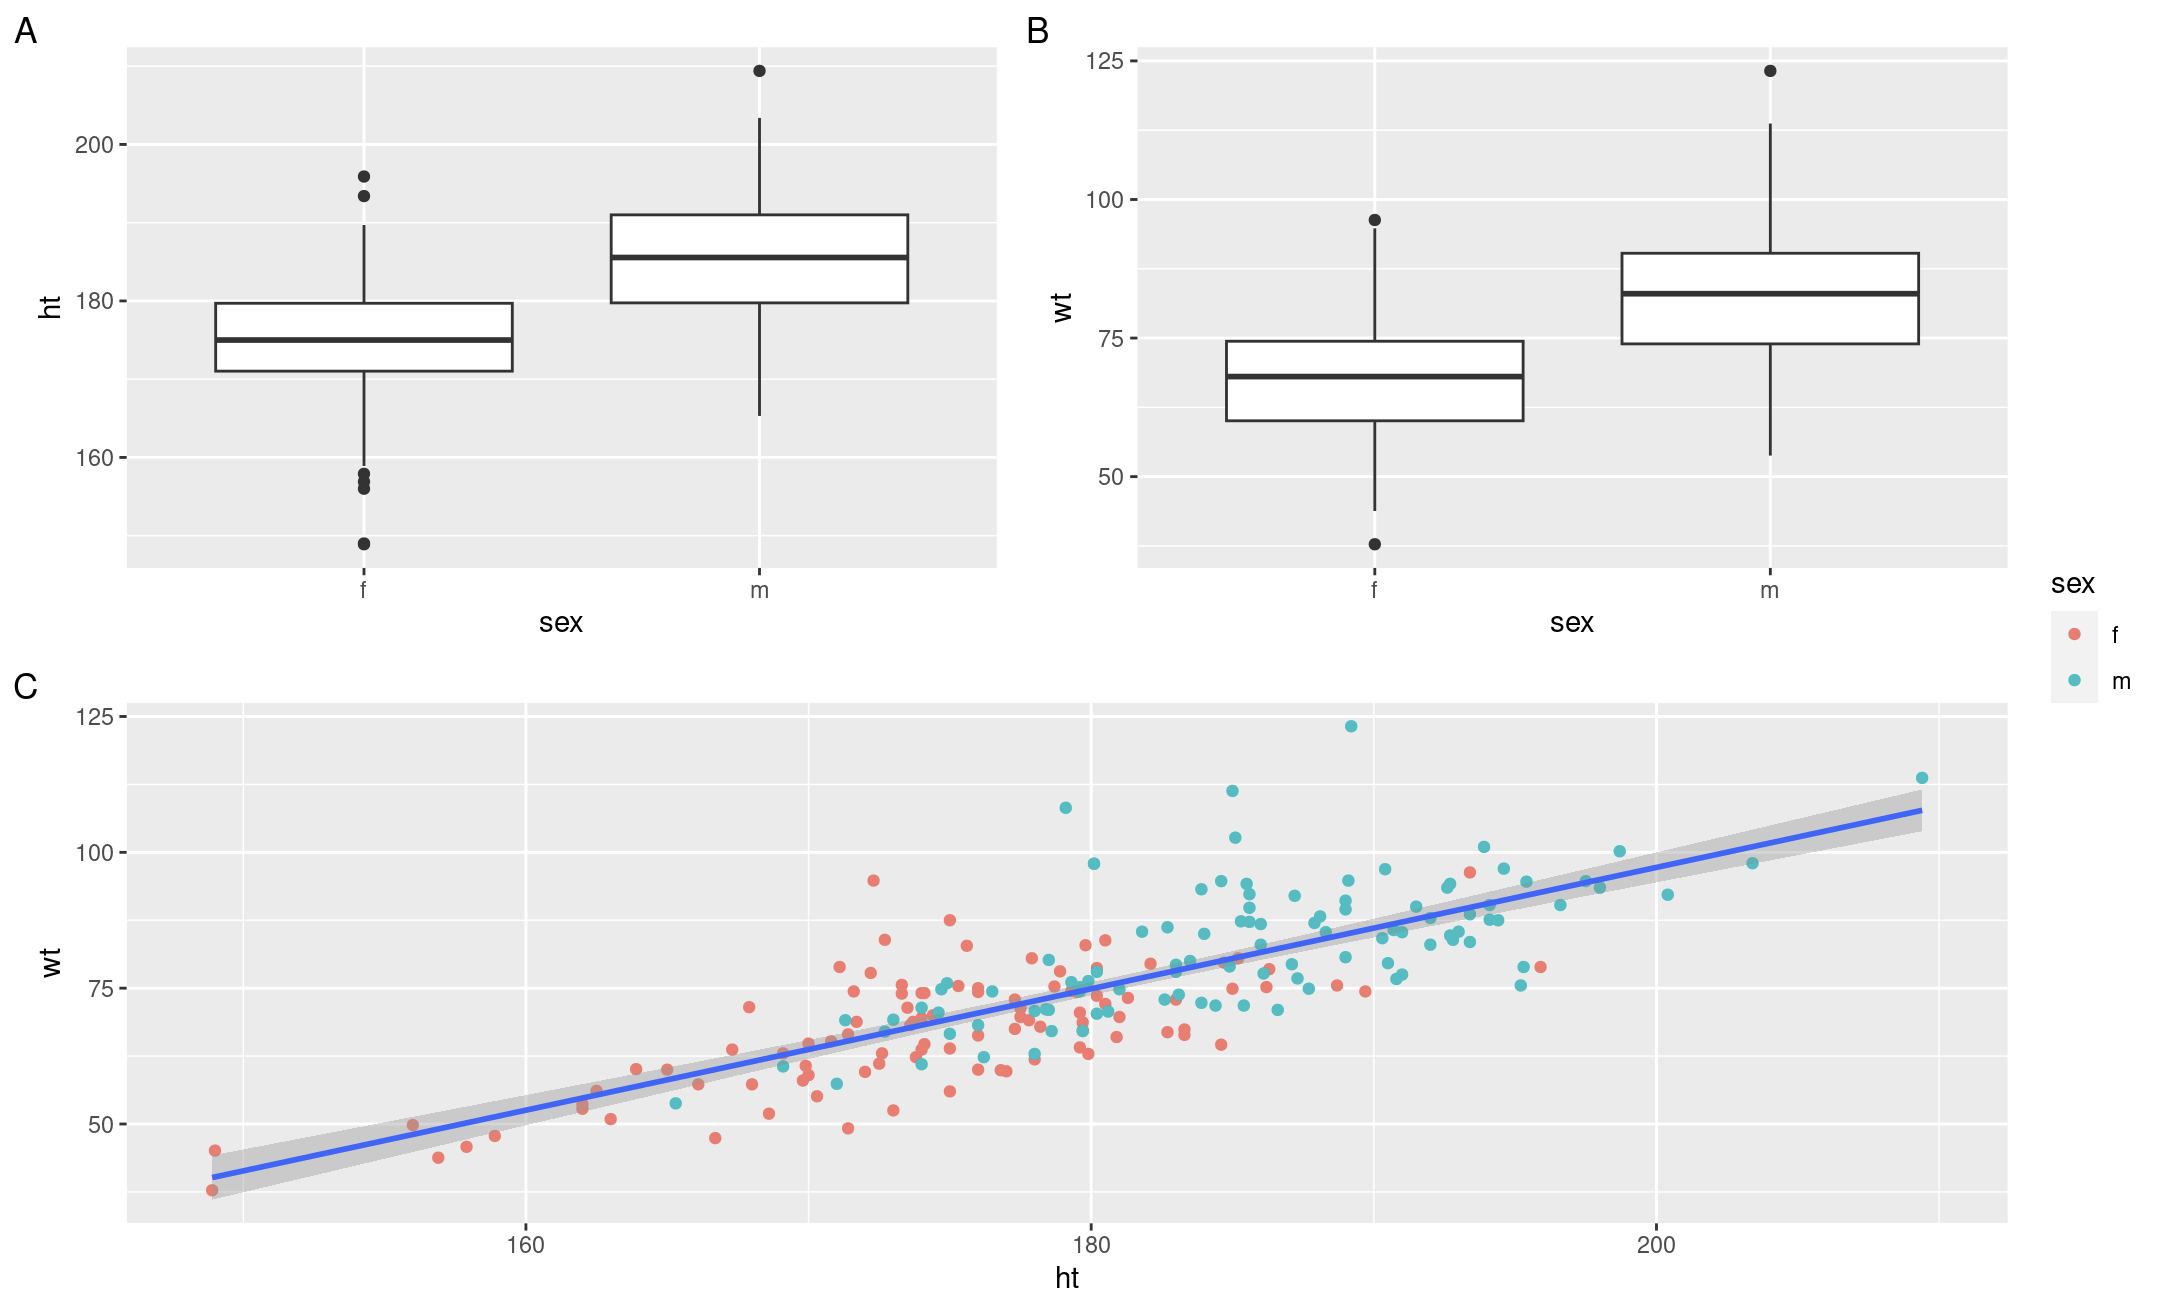
\includegraphics[width=0.9\linewidth]{figures/multipanel} \caption{Results from the patchwork demonstration chunk}\label{fig:unnamed-chunk-78}
\end{figure}

\textless\textless\textless\textless\textless\textless\textless{} HEAD
Have a go at putting some of your report ready plots into a multi-panel figure. Use \texttt{ggsave} to save all of the figures (multi-panel or single-panel). Check your pdf sizes to make sure they are scaled sensibly, you can change the scaling options by looking at the code chunks in Chapter \ref{export}. You can download these pdfs by opening them in browser and clicking the download button in the top right hand corner.
=======
Have a go at putting some of your report ready plots into a multi-panel figure. Use \texttt{ggsave} to save all of the figures (multi-panel or single-panel). Check your pdf sizes to make sure they are scaled sensibly, you can change the scaling options by looking at the code chunks in \textbf{Chapter 12}. You can download these pdfs by opening them in browser and clicking the download button in the top right hand corner.
\textgreater\textgreater\textgreater\textgreater\textgreater\textgreater\textgreater{} 7c875222307693b9fb69a50ba3edddb75a89628b

\hypertarget{analysis-writing}{%
\section{Writing about your analysis}\label{analysis-writing}}

We have done a lot of exploration when it comes to presenting data and performing analysis. But something you will frequently be asked to do throughout your degree, is write about your findings. Here I will cover a few summary point to bare in mind when writing about your analyses.

\begin{itemize}
\tightlist
\item
  Keep it concise - always aim to keep sentences short and snappy when writing in the sciences
\item
  Be specific - make sure it is very clear what it is you are discussing, especially when you have a project with multiple variables
\item
  Keep it biology focused - statistics, be they inferential or descriptive, are helpful when building an argument, you can use them to support your point, but the point should be biology driven.
\item
  \textbf{Always} give a measure of spread, like standard error, when discussing a mean.
\end{itemize}

\textbf{Do} this;

``Male gorillas ate fewer bananas per day (mean ± s.e. = 12.3 ± 1.3) compared to females (mean ± s.e. = 14.7 ± 1.1)''

\textbf{Do NOT} do this;

``The mean was 12.3 for males and 14.7 for females so females ate more bananas.''

This second example makes the entire sentence about the mean values and not about the biological question, which is the difference in bananas eaten by male and female gorillas. It also lacks details like standard deviation or error but discusses a mean which by itself is not very meaningful. The first example was a much more professional and scientifically sound way to report this analysis, using values from the analysis to support the main argument. It will take practice to introduce this writing method into your own work.

You may have noticed that in papers and published reports statistics are reported in a very specific way. When reporting statistics, you should try to state what is shown and then include supporting information, in brackets, from the statistical analysis you have run. When reporting statitics, you should report;

\begin{itemize}
\tightlist
\item
  The statistical test used (e.g.~T-test, ANOVA, etc)
\item
  The test statistic (T value or F value for T-tests or ANOVA)
\item
  Degrees of freedom or some alternative indicator of sample size as recomended by the test run
\item
  p value
\end{itemize}

For example,

\textbf{Do} this;

``Male gorillas ate fewer bananas per day (mean ± s.e. = 12.3 ± 1.3) compared to females (mean ± s.e. = 14.7 ± 1.1) and this difference was significant (T-test, t = -3.7, d.f. = 99, P = 0.035)''

\textbf{Do NOT} do this;

``The mean was 12.3 for males and 14.7 for females so females ate more bananas. The test was significant because p\textless{} 0.05''

This second example is very commonly seen in student work and should be avoided at all costs. The analyst here is asking the reader to accept that there was a statistical difference because p was less than an the arbitrary cut off of 0.05. It gives no evidence to show that this is true. It also creates the impression that the person who conducted the analysis had no understanding of how or why they were analysing the data or what it was they were looking for. The first example is only fractionally longer, but provides much more information to the reader, it is professional and allows the reader to feel confident that the analyst is basing their conclusion on sound scientific and statistical evidence.

\hypertarget{legend2}{%
\subsection{Task 3 - Writing a figure legend}\label{legend2}}

You will often need to construct figure legends, here are a few reminders to bare in mind;

\begin{itemize}
\tightlist
\item
  Table legends go above and figure legends go below
\end{itemize}

Legends \textbf{should};

\begin{itemize}
\tightlist
\item
  Allow the reader to understand the figure without reference to the text, so include information about what is being shown. For example, with a box plot you may wish to say ``The middle line, box and whiskers represent the median, interquartile range and range, respectively.''
\item
  Include info on sample size, study organism (in Latin) and (if relevant, e.g.~ecology) study location and time
\end{itemize}

Legends \textbf{should NOT};

\begin{itemize}
\tightlist
\item
  Include information that is obvious to a scientific audience (e.g.~``a scatter plot to show'' or ``a graph to show'')
\item
  Repeat what's in the figure (e.g.~describe what the colour mean if you also have a key in the figure)
\end{itemize}

With this in mind have a go at writing a figure legend for some of the report ready figures that you made earlier.

\hypertarget{task-4---have-a-go-at-preparing-a-result-section}{%
\subsection{Task 4 - Have a go at preparing a result section}\label{task-4---have-a-go-at-preparing-a-result-section}}

You have some report ready figures and some report ready figure legends now. The next step is to put this together into a result section. Have a think about how you would describe the data you are presenting. It only needs to be a couple of paragraphs. Have a demonstrator check your work.

\hypertarget{wrapping-up-2}{%
\section{Wrapping up}\label{wrapping-up-2}}

This is the final content driven Data Sciences workshop. This term we have been slowly progressing through the complete workflow of the analysis of a small data set. We started by importing, checking and cleaning our data, we then did some data exploration and made some exploratory plots before using descriptive and inferential statistics to investigate differences and relationships in more depth. Finally, today, we have looked at the processes of selecting and preparing plots for presentation and how to write about our findings. The next chapter contains the Data Sciences portion of the Skills for Biologists portfolio task, which is the summative assignment for this term. There is one more workshop which is a drop in session, you can get help on your code at this session, but we cannot help with other aspects of your assignment.

\hypertarget{before-you-leave-9}{%
\section{Before you leave!}\label{before-you-leave-9}}

Log out of posit Cloud and make sure you save your script!

\hypertarget{references-10}{%
\section{References}\label{references-10}}

Pedersen, T. L. (2020). Patchwork: The composer of plots. \url{https://CRAN.R-project.org/package=patchwork}
Telford, R.D. and Cunningham, R.B. 1991. Sex, sport and body-size dependency of hematology in highly trained athletes. Medicine and Science in Sports and Exercise 23: 788-794. Pedersen, T. L. (2020). Patchwork: The composer of plots. \url{https://CRAN.R-project.org/package=patchwork}
Telford, R.D. and Cunningham, R.B. 1991. Sex, sport and body-size dependency of hematology in highly trained athletes. Medicine and Science in Sports and Exercise 23: 788-794.
Wickham, Hadley, Mara Averick, Jennifer Bryan, Winston Chang, Lucy D'Agostino McGowan, Romain François, Garrett Grolemund, et al.~2019. ``Welcome to the tidyverse.'' Journal of Open Source Software 4 (43): 1686. \url{https://doi.org/10.21105/joss.01686}.
Wickham, Hadley, Winston Chang, Lionel Henry, Thomas Lin Pedersen, Kohske Takahashi, Claus Wilke, Kara Woo, Hiroaki Yutani, and Dewey Dunnington. 2021. Ggplot2: Create Elegant Data Visualisations Using the Grammar of Graphics. \url{https://CRAN.R-project.org/package=ggplot2}.

\hypertarget{portfolio-tasks}{%
\chapter{Portfolio Tasks}\label{portfolio-tasks}}

\hypertarget{background}{%
\section{Background}\label{background}}

The data you will be analysing focus' on parasite abundance in \emph{Corydoras} catfish.

\begin{figure}
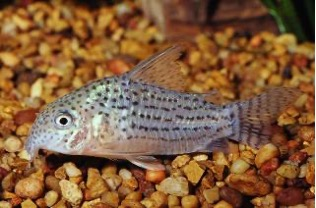
\includegraphics[width=0.9\linewidth]{figures/cory} \caption{*Corydoras araguaiaensis*}\label{fig:unnamed-chunk-79}
\end{figure}

\emph{Corydoras} catfishes were collected from Brazil and identified. Each fish belonged to one of two species that are very similar in life history but have dramatically different genome sizes. \emph{Corydoras araguaiaensis} is a polyploid species (probable tetraploid), and \emph{Corydoras maculifer} is a diploid species. The two species are müllerian mimics and coexist, sharing a niche, so environmentally they have had very similar experiences.

This prediction was that polyploid fish may carry a higher number of different immune alleles and therefore may be better able to resist parasites than the diploid species. The fish were dissected and number of parasites found within each individual was counted.

\hypertarget{the-data-1}{%
\section{The data}\label{the-data-1}}

The data you have been provided with can be found \href{https://downgit.github.io/\#/home?url=https://github.com/ellenbell/4008Y/blob/main/data/catfish_parasite_data.csv}{here}, it is also on blackboard should the download link prove troublesome. Go to the Workbook and Data Sets folder in the Data Sciences Learning Module in your Skills module blackboard page, the file is called \texttt{catfish\_parasite\_data.csv}.

The data consist of four variables;

\begin{enumerate}
\def\labelenumi{\arabic{enumi})}
\tightlist
\item
  sample - this is simply a sample ID with values ranging from 1-61
\item
  length\_mm - standard length in millimetres. Standard length is a method of measurement for fish and is recorded as the distance from the tip of the snout to the base of the tail.
\item
  species - either the polyploid \emph{C. araguaiaensis} (A) or the diploid \emph{C. maculifer} (M)
\item
  parasite\_count - a measure of total parasites counted per individual
\end{enumerate}

This data set was adapted from Bell et al., 2020.

\hypertarget{the-tasks}{%
\section{The tasks}\label{the-tasks}}

You will need to produce a series of plots to answer the questions in \textbf{Exercise 1} and present them at publication standard in a multi-panel layout alongised a figure legend. You will then be required to present your script for the second part of this assessment in \textbf{Exercise 2}.

\hypertarget{exercise-1---figure-and-figure-legend}{%
\subsection{Exercise 1 - Figure and figure legend}\label{exercise-1---figure-and-figure-legend}}

You wish to know if there is a link between genome size and parasite load in \emph{Corydoras} catfishes, but you also want to make sure and show that there are no confounding variables (like size) affecting any conclusions you draw from your analysis. So you ask three questions of your data;

\begin{enumerate}
\def\labelenumi{\arabic{enumi})}
\tightlist
\item
  Is there a difference in length between \emph{C. araguaiaensis} and \emph{C. maculifer}?
\item
  Is there a difference in parasite abundance between \emph{C. araguaiaensis} and \emph{C. maculifer}?
\item
  Is there a relationship between length and parasite abundance in \emph{C. araguaiaensis} and \emph{C. maculifer}?
\end{enumerate}

Set up a new R studio project, import the catfish\_parasites data and make sure it is clean and tidy. Complete all the checks that you did in Chapter \ref{data-setup} and then you can start exploring the data as you did in Chapter \ref{data-setup} and \ref{stats}. When you are satisfied with the data quality and appearance you can begin to answer the questions above. Construct a plot to address each of these questions. I suggest a plot per question. Make them visually pleasing and then combine the three plots into a multi-panel figure as you did in Chapter \ref{reporting}. Export this as a pdf (see Chapter \ref{export}). You will be able to download this pdf to your own computer when you are happy with it, instructions on how to do this are in Chapter \ref{formative}.

Now you will need to copy your figure into a word document and write a suitable figure legend. We have discussed figure legends in lectures and in Chapters \ref{formative} and \ref{legend2} we have also explored how to report results in Chapter \ref{analysis-writing}. So now write a clear but concise figure legend underneath your newly made figure.

\hypertarget{exercise-2---code}{%
\subsection{Exercise 2 - Code}\label{exercise-2---code}}

As before, during the formative, we require you to upload the script you have created to analyse the \texttt{catfish\_parasites.csv} dataset. I strongly recommend keeping your script nice and clean and tidy and well commented throughout your \texttt{catfish\_parasite} analysis and have it saved nicely in your \texttt{scripts} folder. If you do then this step will be super easy! You simply need to download your script using the same method described above in Chapter \ref{formative}.

\hypertarget{submission}{%
\subsection{Submission}\label{submission}}

If you go to the Data Sciences Learning Module in the BIO-4008Y page of blackboard you will see a link to PebblePad. If you follow this link you should be automatically taken to the Data Sciences portfolio. You will see there are two pages to the portfolio, at this stage you only need to complete the \texttt{Summative} page. You will see there are a number of tick boxes to help guide you through what our expectations are from your work here. There are then two places to upload your work, one for your figure and figure legend and the other for your script. Upload the corresponding documents where required.

You may notice that there is a check box where you will need to assert that this is your own work. Once this is done you can scroll down and you will be able to mark the page as complete. Once you have marked your page as complete you can consider it submitted.

\begin{quote}
Top tip - as you scroll down the page you can see that there is a marking rubric included, these are the criteria under which we will be marking your work, a similar one has been created for the summative page as well.
\end{quote}

Good luck everyone! The final workshop in Week 8 will be a drop in session, so if you are really stuck do feel free to pop by. We can help you with fixing code but cant give you more feedback then that.

\hypertarget{references-11}{%
\section{References}\label{references-11}}

Bell, E., Cable, J., Oliveira, C., Richardson, D., Yant, L. \& Taylor, M. (2020); Help or Hindrance? The evolutionary impact of whole-genome duplication on immunogenetic diversity and parasite load. Ecology and Evolution. 10 (24). 13949-13956.

\end{document}
